\documentclass[11pt,a4paper,twoside,openany]{book}
\usepackage{lifeos}
\usepackage{pgfplots}\pgfplotsset{compat=1.17}
\usepackage{circuitikz}
\usepackage{graphicx}
\usepackage[font=small,labelfont=bf]{caption}
\usepackage{subcaption}
\usepackage{siunitx}
\usepackage{makeidx}\makeindex
\setlifeostitle{BOOK TITLE}
\setcounter{tocdepth}{1}

\begin{document}
\frontmatter
\pagestyle{empty}
\makecover{BOOK TITLE}{Subtitle}{Study textbook}
\newpage\pagestyle{fancy}
\tableofcontents
\mainmatter
% Chapter 1 -- Electricity, circuits and the workbench
\chapter{Electricity, circuits and the workbench}
\label{ch:workbench}

This chapter builds the vocabulary and the bench habits that every later chapter
takes for granted. It answers four questions: what electricity \emph{is}
(as much as an engineer needs to know), what voltage, current and resistance
measure, how to read a schematic and turn it into a shopping list, and which of
the things on a workbench can hurt you. When you finish it you should be able
to: translate a simple schematic into parts and measurements, use a multimeter
for the three basic measurements without blowing its fuse, say precisely what
this book will and will not ask you to touch, and check whether your computer
already has the tools this book needs.

\section{What electricity is}
\label{sec:charge}

Strip everything away and electricity starts with one observation: objects can
push and pull on each other without touching. Rub a balloon on your hair and it
will pick up scraps of paper from a table. Something invisible reached out and
grabbed them. That something is \emph{charge}\index{charge|textbf}: a basic
property of matter, like mass, that some particles carry and others do not.
Charge comes in two flavours that attract each other and repel their own kind,
which we call positive and negative — the names are a bookkeeping device, not a
value judgment. The electron carries one fixed small negative charge; the proton
carries the same amount positive. That fixed amount, $e \approx
1.602\times10^{-19}$~coulombs\index{coulomb}, is the smallest packet of free
charge we ever deal with. Ordinary matter contains roughly equal numbers of
protons and electrons and so looks neutral; ``charging'' an object means
unbalancing that equality slightly.

A charge creates a disturbance in the space around it — an \emph{electric
field}\index{electric field|textbf} — and other charges feel that disturbance as
a force. We almost never draw the field itself in this book, but it is what
makes everything else work, so we define the quantity that packages it:
\emph{voltage}\index{voltage|textbf} (also called \emph{potential
difference}\index{potential difference}). Voltage is the field's push measured
as energy: the voltage between two points is the energy needed to move one unit
of charge from one to the other,
\[
  V = \frac{W}{q}, \qquad \text{1 volt} = \text{1 joule per coulomb}.
\]
A ``\qty{9}{\volt} battery'' is a device that gives each coulomb of charge
\qty{9}{\joule} of push between its terminals. Voltage is always measured
\emph{between two points}; the phrase ``the voltage at this wire'' is shorthand
for ``the voltage between this wire and whatever we agreed to call zero,'' and
that agreed-zero is the \emph{ground}\index{ground} node we draw at the bottom
of every schematic.

\begin{remark}[What we are skipping]
That paragraph is honest but thin. The full story is electromagnetic field
theory — fields propagate, wires are not the whole circuit, and at high
frequencies our tidy model breaks. For the circuits in this book (centimetres
across, signals slower than tens of megahertz) the \emph{lumped} model — every
property lives inside components connected by ideal wires — is accurate to far
better than the tolerance of any part you can buy. Where it stops being true
(radio, very fast digital edges, mains safety) we say so at the point it matters
rather than here. If you want the real derivations, a free calculus-based
physics text covers charge, field and potential properly \cite{openstaxv2}.
\end{remark}

\begin{figure}[htbp]
\centering
% Figure: charge -> moving charge -> current  (ch01)
\begin{tikzpicture}[scale=0.9,font=\small]
  % --- left: one atom ---
  \begin{scope}
    \fill[accentsoft] (0,0) circle (0.32);
    \node at (0,0) {\tiny +};
    \draw[slate!70] (0,0) circle (0.85);
    \draw[slate!70] (0,0) circle (1.25);
    \fill[ink] (0.85,0) circle (0.055) node[below right,xshift=1pt,yshift=-1pt]{\scriptsize $-$};
    \fill[ink] (-0.5,0.7) circle (0.055);
    \fill[ink] (-1.05,-0.66) circle (0.055);
    \node[align=center] at (0,-1.75) {\scriptsize matter: a few\\[-1pt]\scriptsize spare electrons};
  \end{scope}
  % --- arrow ---
  \draw[->,thick,accent] (1.7,0) -- (3.1,0);
  % --- middle: a wire full of drifting electrons ---
  \begin{scope}[xshift=3.4cm]
    \draw[rounded corners,thick] (0,-0.55) rectangle (4.6,0.55);
    \foreach \x/\y in {0.35/0.15, 0.8/-0.3, 1.25/0.35, 1.7/-0.1, 2.2/0.25, 2.7/-0.35, 3.15/0.1, 3.6/-0.2, 4.05/0.3, 4.35/-0.05}
      \fill[ink] (\x,\y) circle (0.05);
    \foreach \x in {0.5,1.5,2.5,3.5}
      \draw[->,slate] (\x,-0.75) -- (\x+0.5,-0.75);
    \node at (2.3,-1.35) {\scriptsize a wire: charge drifting along it};
    \node[slate] at (2.3,-1.05) {\scriptsize electron drift $\longrightarrow$};
  \end{scope}
  % --- right: the measure ---
  \begin{scope}[xshift=8.6cm]
    \draw[->,very thick,accent] (0,0) -- (1.6,0) node[right]{$I$};
    \node[align=center] at (0.8,-1.35) {\scriptsize current: how much\\[-1pt]\scriptsize charge per second};
  \end{scope}
\end{tikzpicture}

\caption{Read left to right: atoms are mostly neutral; a metal wire contains
electrons that are free to drift; a battery (the field source) makes them drift
in one direction. That drift \emph{is} the current. Notice what is \emph{not}
shown: the battery does not inject electrons into an empty pipe — the electrons
are already in the wire; the source only organises their motion.}
\label{fig:charge}
\end{figure}

\section{Current}
\label{sec:current}

A metal wire is full of electrons that belong to no particular atom and drift
randomly, as much left as right: no net motion, no current. Put a source across
the wire — a field along it — and the random drift gains a small organised
component in one direction. That net flow of charge is
\emph{current}\index{current|textbf}:
\[
  I = \frac{\Delta Q}{\Delta t}, \qquad \text{1 ampere} = \text{1 coulomb per second}.
  \index{ampere}
\]
One amp is roughly $6\times10^{18}$ electrons per second squeezing through a
cross-section of wire. You never count electrons; the meter does it for you by
watching the field they drag with them.

It is worth calibrating the unit with real numbers. The LED we light in this
chapter runs at about \qty{20}{\milli\ampere}. A phone charger supplies
\qtyrange{1}{2}{\ampere}. The LED strips in cheap room lighting draw a few
hundred milliamps. A bolt of lightning peaks in the tens of kiloamps — which is
why ``it is only a little circuit'' is a sentence that needs a voltage and a
current attached before it means anything.

Two conventions matter immediately. First, current is a \emph{signed}
quantity with an arrow: we pick a direction for the arrow, compute or measure
$I$, and a negative answer means the flow goes opposite to our arrow. Second —
and this trips up every beginner — the arrow points the way \emph{positive}
charge would move, which is opposite to the actual electron drift. That
historical quirk is Section~\ref{sec:conventions}'s whole topic; for now just
note that the arrow in Figure~\ref{fig:first} points the engineering way.

\section{Resistance and the resistor}
\label{sec:resistance}

Push charge through almost any material and it meets drag: the moving electrons
scatter off the lattice and hand their energy back as heat. The measure of that
drag is \emph{resistance}\index{resistance|textbf},
\[
  R = \frac{V}{I}, \qquad \text{1 ohm} = \text{1 volt per ampere}.
\]
A material with twice the resistance needs twice the voltage to push the same
current. Copper wire has nearly none (milliohms per metre); the carbon film
inside a quarter-watt \emph{resistor}\index{resistor|textbf} — the single most
common component in this book — is manufactured to a precise value from
fractions of an ohm to tens of megohms.

The relationship $V = I\,R$ is \emph{Ohm's law}\index{Ohm's law}: one equation
linking all three quantities, so that knowing any two fixes the third. We use
it lightly this chapter (to estimate a battery's life and to \emph{pose} the
problem in Example~\ref{ex:led}), and Chapter~2 turns it into a working tool.
\begin{remark}
``Ohm's law'' is really an empirical pattern, not a law of nature — it holds
beautifully for resistors and not at all for LEDs, transistors or arcs. The
components that break it are exactly the interesting ones; that is Chapters 5
and 6.
\end{remark}

Resistor values are printed as coloured bands\index{resistor!colour code} — a
holdover from when components were too small to label. You need only the
four-band reading: first two bands are digits, the third is the multiplier
(power of ten), the fourth is tolerance. Table~\ref{tab:bands} gives the digits;
Exercise~\ref{ex:easy-bands} drills it.

\begin{table}[htbp]
\centering\small
\begin{tabularx}{\linewidth}{lY}
\toprule
\thead{Colour} & \thead{Digit (multiplier $10^{n}$)}\\
\midrule
Black & 0\\
Brown & 1\\
Red & 2\\
Orange & 3\\
Yellow & 4\\
Green & 5\\
Blue & 6\\
Violet & 7\\
Grey & 8\\
White & 9\\
\midrule
Gold (4th band) & tolerance $\pm 5\%$\\
Silver (4th band) & tolerance $\pm 10\%$\\
\bottomrule
\end{tabularx}
\caption{The only colour-code facts this book needs: digit values and the two
common tolerance bands. Brown--black--red--gold $=1,0,\times10^{2},\pm5\% =
\qty{1}{\kilo\ohm}$. Notice you read \emph{toward} the gap between the digit
bands and the spaced-off tolerance band.}
\label{tab:bands}
\end{table}

Values span so many orders of magnitude that electronics runs on
\emph{engineering prefixes}\index{metric prefixes} in steps of $10^{3}$:
milli~m ($10^{-3}$), micro~µ (``u'' in plain ASCII, $10^{-6}$), nano~n
($10^{-9}$), pico~p ($10^{-12}$), kilo~k ($10^{3}$), mega~M ($10^{6}$). A
``4k7'' resistor is \qty{4.7}{\kilo\ohm} $= \qty{4700}{\ohm}$; a ``100 nF''
capacitor is \qty{100}{\nano\farad} $= \qty{0.1}{\micro\farad}$. Datasheets,
schematics and meters each pick different prefixes, so fluency is not optional.
The chapter ships a tiny converter (Listing~\ref{lst:prefix}) you can check your
mental arithmetic against.

\begin{exercise}[easy]
Convert: \qty{0.05}{\ampere} to milliamps; \qty{4.7}{\kilo\ohm} to ohms;
\qty{0.0000001}{\farad} to nanofarads. Then run \texttt{prefix.py} and check.
\end{exercise}

Before leaving the three quantities, one deserved warning about how you will
hear them explained elsewhere. The \emph{water analogy}\index{water analogy} —
voltage is pressure, current is flow, a resistor is a narrow pipe — is the
standard pictorial model, and it is not useless: it correctly predicts that
more pressure drives more flow and that pinching the pipe reduces it.
Figure~\ref{fig:analogy} puts it beside the honest version. It fails in
exactly the places where intuition matters most (a cut wire does not ``leak''
current onto the bench; a battery does not inject anything) — which is why
this book uses it as a first sketch and then abandons it.
Exercise~\ref{ex:water} asks you to catalogue the failures properly.

\begin{figure}[htbp]
\centering
% Figure: the water analogy, honestly framed (ch01)
\begin{tikzpicture}[scale=0.88,font=\small]
  % ---------- left: water ----------
  \begin{scope}
    % pump
    \draw[thick] (0,0) circle (0.5);
    \node at (0,0) {\scriptsize pump};
    % pipe loop
    \draw[very thick,accent] (0,0.5) -- (0,1.3) -- (4.2,1.3) -- (4.2,0.2);
    \draw[very thick,accent] (0,-0.5) -- (0,-1.3) -- (4.2,-1.3) -- (4.2,-0.2);
    % constriction
    \draw[very thick,accent] (4.2,0.2) -- (4.2,-0.2);
    \draw[thick,fill=graybg] (4.2,0.2) -- (4.55,0.08) -- (4.55,-0.08) -- (4.2,-0.2) -- cycle;
    % flow arrows
    \draw[->,thick] (1.4,1.05) -- (2.2,1.05);
    \draw[->,thick] (2.8,-1.05) -- (2.0,-1.05);
    \node[align=left,anchor=west] at (5.0,0.55) {\scriptsize pump $\approx$ source};
    \node[align=left,anchor=west] at (5.0,0.1) {\scriptsize pressure $\approx$ voltage};
    \node[align=left,anchor=west] at (5.0,-0.35) {\scriptsize constriction $\approx$ resistor};
    \node[align=left,anchor=west] at (5.0,-0.8) {\scriptsize flow $\approx$ current};
    \node at (2.3,-2.0) {\scriptsize\itshape the analogy};
  \end{scope}
  % ---------- right: where it breaks ----------
  \begin{scope}[yshift=-3.4cm]
    \node[align=left,anchor=north west,text width=13.2cm] at (-0.4,0)
      {\scriptsize\textbf{Where it breaks:} cut a pipe and the water pours out; cut a wire and
       charge simply stops. There is no ``leak'' of charge, nothing pushes sideways, and the
       pressure exists \emph{between} two points, not inside one point. Keep the picture for
       intuition in this chapter; drop it the moment it argues back.};
  \end{scope}
\end{tikzpicture}

\caption{The water analogy, kept honest. Left: the picture as usually drawn
(pump = battery, pipe = wire, constriction = resistor). Right: what each piece
actually is — pressure is energy per charge, flow is charge per second, the
``constriction'' is energy lost to lattice collisions. The analogy survives
Ohm's-law arithmetic and dies at the physics: a cut pipe leaks, a cut wire
just stops.}
\label{fig:analogy}
\end{figure}

\section{A complete circuit — and the schematic as the real object}
\label{sec:schematic}

Current flows only in loops. Three things must exist for it to do so: a
\emph{source} that provides the push (a battery, a USB port, a power supply), a
\emph{conducting path} that carries the flow (wire, plus the components in the
way), and a route \emph{back to the source}\index{circuit!closed loop}. Break
the loop anywhere and the current stops everywhere — instantly, throughout the
whole loop. That is the entire operating principle of a switch, and it is the
reason one broken wire can kill a whole circuit.

Figure~\ref{fig:first} shows the smallest circuit that does something useful:
a \qty{5}{\volt} source, a resistor, and a light-emitting diode (LED). The
schematic\index{schematic|textbf} — the drawn map of symbols and wires — is not
an illustration of the circuit; in every practical sense it \emph{is} the
circuit. The copper and plastic are just a heavy, solderable printout of the
schematic. This is why we insist all circuits in this book be drawn properly
(with \texttt{circuitikz}) rather than photographed.

\begin{figure}[htbp]
\centering
% Figure: first real schematic -- USB 5V, resistor, LED (ch01)
\begin{circuitikz}[scale=1.0,transform shape]
  \draw (0,0) node[ground]{};
  \draw (0,0) to[battery1,l_=\qty{5}{\volt},invert] (0,2.4);
  \draw (0,2.4) to[R,l=$R$] (3.2,2.4);
  \draw (3.2,2.4) to[leD,l=LED] (3.2,0) node[ground]{};
  % current arrow on top wire
  \draw[->,thick,accent] (0.6,2.85) -- (1.8,2.85) node[midway,above]{$I$};
  % node dots (the two wires between parts are "the same node")
  \node[circ] at (0,2.4) {};
  \node[circ] at (3.2,0) {};
\end{circuitikz}

\caption{Our first real schematic. Read it as a loop, not a picture: leave the
top of the source at $+\qty{5}{\volt}$, pass through $R$ (which will limit the
current), through the LED (which lights if the current is right), down to the
ground symbol and back into the bottom of the source. The arrow marks the
\emph{chosen} current direction (Section~\ref{sec:conventions}). Notice the LED
symbol: diode triangle plus two small arrows = ``the diode that emits.''}
\label{fig:first}
\end{figure}

Here is the subtle point beginners miss. The schematic records
\emph{connections}, not \emph{locations}. Two points joined by a drawn wire (or
marked with the same net name) are the same electrical object — the same
\emph{node}\index{node|textbf}. Points merely near each other on paper are
nothing. Figure~\ref{fig:topology} draws the same circuit twice: tidy, and
stretched into an ugly pose. Electrically they are identical, because every
node contains the same component leads. Reading schematics as
\emph{topology}\index{topology} — who is connected to whom, never where they
sit — is the skill this section exists to install. We will reuse it
mercilessly when schematics get big in Chapter~17.

\begin{figure}[htbp]
\centering
% Figure: same topology, different geography (ch01)
\begin{circuitikz}[scale=0.9,transform shape]
  % (a) canonical loop
  \begin{scope}
    \draw (0,0) node[ground]{};
    \draw (0,0) to[battery1,l_=\qty{5}{\volt},invert] (0,2.2);
    \draw (0,2.2) to[R,l=$R$] (2.8,2.2);
    \draw (2.8,2.2) to[leD,l=LED] (2.8,0) node[ground]{};
    \node at (1.4,-0.9) {\scriptsize (a) the tidy drawing};
  \end{scope}
  % (b) same netlist, bent around
  \begin{scope}[xshift=5.6cm]
    \draw (0,0) node[ground]{};
    \draw (0,0) to[battery1,l_=\qty{5}{\volt},invert] (0,2.2);
    \draw (0,2.2) -- (1.6,2.2) -- (1.6,0.9) to[R,l=$R$] (3.4,0.9);
    \draw (3.4,0.9) -- (3.4,1.8) to[leD,l=LED] (4.9,1.8) -- (4.9,0) node[ground]{};
    \node at (2.45,-0.9) {\scriptsize (b) bent, stretched --- still the same circuit};
  \end{scope}
\end{circuitikz}

\caption{Same circuit, two drawings. To prove (a) $\equiv$ (b), list what is
attached to each node: node A holds source-$+$ and resistor lead 1; node B holds
resistor lead 2 and LED anode; node C holds LED cathode and source$-$. The lists
match, so the circuits are the same. The drawing changed; the
\emph{connections} — the only thing the circuit cares about — did not.}
\label{fig:topology}
\end{figure}

\begin{example}[From schematic to shopping list]
\label{ex:partslist}
\emph{Problem.} Turn Figure~\ref{fig:first} into a parts order.\par
\emph{Strategy.} Walk the schematic component by component, not wire by wire.
For each symbol write the thing to buy and the value or rating written beside
it. Wires and ground symbols buy nothing — they come free with the breadboard
and cables.\par
\emph{Solution.}
\begin{itemize}
\item one \qty{5}{\volt} source — a USB cable or a \qty{5}{\volt} supply;
\item one resistor, value $R$ — value still undetermined
(Example~\ref{ex:led} is about exactly this gap);
\item one LED, any colour, standard \qty{5}{\milli\metre} or
\qty{3}{\milli\metre} package;
\item means of connecting: breadboard + jumper wires (Section~\ref{sec:kit}).
\end{itemize}
\emph{Notice:} the schematic already told us everything except one number —
which is the kind of gap a circuit diagram is supposed to leave for analysis.
\end{example}

\begin{example}[The LED question, posed on purpose]
\label{ex:led}
\emph{Problem.} The LED in Figure~\ref{fig:first} wants about \qty{2}{\volt}
across itself and shines nicely at \qty{10}{\milli\ampere}, burns at
\qty{30}{\milli\ampere}. The source is \qty{5}{\volt}. What should $R$
be?\par
\emph{Strategy.} Take stock of what each quantity does. The source fixes the
total push: \qty{5}{\volt}. The LED spends about \qty{2}{\volt} of it (a fact of
diode physics we take on trust until Chapter~5). The resistor must drop the
rest, and the same current must pass through everything in a single loop. So
the missing ingredient is a law that links the resistor's voltage share to the
current through it — which is $V = IR$. We \emph{have} that law already; what
we are missing is practice using it and one bookkeeping rule (Kirchhoff's
voltage law) that makes ``the rest'' precise.\par
\emph{Solution.} Held for Chapter~2, where it becomes a one-line computation.
The point of posing it now: you can already see that $R$ exists to dispose of a
voltage difference and to choose a current — the two jobs resistors do all book
long.
\end{example}

\section{Two conventions for direction}
\label{sec:conventions}

Benjamin Franklin guessed the sign of charge wrongly, and by the time electrons
were identified the convention was set: circuit arrows point the way
\emph{positive} charge would flow — \emph{conventional
current}\index{conventional current|textbf}. Electrons, being negative, drift
the other way — \emph{electron flow}\index{electron flow}.

Nothing about this is optional to get right, because everyone — every
datasheet, every schematic, every simulator — uses conventional current. When
someone (or a YouTube video) insists on electron flow, mentally flip every
arrow; the numbers and the physics are unaffected. The failure mode is not
choosing the ``wrong'' convention but switching conventions
\emph{mid-argument}: if you label an arrow one way and reason about electrons
the other way, signs invert silently and the sums stop making sense. Pick
conventional current and stay there; this book never leaves it.

\begin{principle}[Arrows are reference directions]
Draw the arrow whichever way is convenient. A positive computed value means
flow along your arrow; negative means against it. You do not have to guess the
``true'' direction first — the sign will tell you.
\end{principle}

\section{The multimeter}
\label{sec:dmm}

The \emph{multimeter}\index{multimeter|textbf} (or DMM, for digital
multimeter) is the one instrument this book treats as essential. It measures
the three quantities of Sections~1--3 and nothing else we need. Everything else
in electronics is learned through it. Figure~\ref{fig:dmm} shows a typical
unit.

\begin{figure}[htbp]
\centering
% Figure: a multimeter -- dial and probe jacks (ch01)
\begin{tikzpicture}[scale=0.95,font=\small]
  % body
  \draw[thick,rounded corners=8pt] (-2.3,-3.4) rectangle (2.3,3.4);
  % screen
  \draw[thick,fill=graybg] (-1.4,2.35) rectangle (1.4,3.05);
  \node at (0,2.7) {\scriptsize\texttt{1.990}};
  % dial
  \draw[thick] (0,0.35) circle (1.5);
  \fill[accentsoft] (0,0.35) circle (1.18);
  % needle
  \draw[thick,accent,->] (0,0.35) -- (210:1.05);
  \fill[accent] (0,0.35) circle (0.09);
  % dial markings around
  \foreach \a/\t in {150/{V$\sim$}, 120/{V\textbf{---}}, 90/{$\Omega$}, 60/{mA}, 30/{10\,A}, 0/{OFF}, -30/{cont.}, -60/{CAP}}
    \node[font=\scriptsize] at (\a:1.95) {\t};
  % jacks
  \draw[thick,fill=white] (-1.3,-2.3) circle (0.32) node[below,yshift=-7pt]{\scriptsize 10\,A};
  \draw[thick,fill=white] (0,-2.3) circle (0.32) node[below,yshift=-7pt]{\scriptsize COM};
  \draw[thick,fill=white] (1.3,-2.3) circle (0.32) node[below,yshift=-7pt]{\scriptsize V$\Omega$};
  % probes
  \draw[very thick] (-1.6,-2.9) -- (-2.5,-4.3) node[pos=1.05,below]{\scriptsize red};
  \draw[very thick] (0,-2.62) -- (-0.4,-4.4) node[pos=1.05,below]{\scriptsize black};
  \node[slate] at (0,-5.1) {\scriptsize red into V$\Omega$ for volts and ohms; the 10\,A jack is for current only};
\end{tikzpicture}

\caption{A typical multimeter. Three things to notice. (1)~The dial divides the
world into ranges: $\mathrm{V}\!\sim$ (AC volts — never used in this book),
$\mathrm{V}\!\text{-}\!\!\cdot$ (DC volts), $\Omega$ (resistance), mA (current),
10\,A (the big current range), plus extras (continuity beeper, capacitance).
(2)~Three jacks: COM is where the black probe always lives; V$\Omega$ is red for
volts, ohms and small currents; 10\,A is a separate, typically \emph{unfused}
path for large currents. (3)~The screen reads the number \emph{in the selected range's units} —
``1.990'' on the 2\,V range means \qty{1.990}{\volt}, on the mA range
\qty{1.990}{\milli\ampere}.}
\label{fig:dmm}
\end{figure}

The three measurements differ in a way that matters physically, and the
difference explains every DMM accident:

\begin{itemize}
\item \textbf{Voltage} is a \emph{difference between two points}. To measure
it you touch the two probes to the two points — the meter is in
\emph{parallel}\index{multimeter!measuring voltage} with whatever is there.
The circuit does not change; you added an observer, not a wire. Inside the
meter is a very large resistance ($\sim\qty{10}{\mega\ohm}$), so almost no
current diverts into it. Voltage measurement is the safe, always-allowed move.
\item \textbf{Current} is a \emph{flow through a point}. To measure it you must
put the meter \emph{into} the path — break the circuit\index{multimeter!measuring current}
and bridge the gap with the probes, so all the circuit's current passes through
the meter. Inside it is a very \emph{small} resistance (a shunt). This is the
measurement that changes the circuit and the one beginners fry meters with.
\item \textbf{Resistance} is measured with the circuit \emph{unpowered}: the
meter sends out its own small test current and reads the resulting voltage.
Measuring resistance on a live circuit gives wrong numbers at best.
\end{itemize}

\begin{tripwire}[The fuse-blower]
Red probe in the current jack + probes across a voltage source = a short
circuit through the meter's (very small) input resistance. On most meters the
mA jack is the fused one — a sacrificial fuse dies for your mistake; the
10\,A jack is typically \emph{unfused}, so the same mistake there can kill
the meter itself, not to mention the circuit you shorted. Make a habit: \emph{after} a
current measurement, the red probe goes back to V$\Omega$ before anything else
is touched. We will never again let it live in the current jack when idle.
\end{tripwire}

\begin{tripwire}[``OL'' is an answer]
On a resistance or voltage range, an ``OL''/``1\ \ '' display means
\emph{over-range}, not zero and not broken: the value exceeds what that range
can show (or the path is genuinely open). On the mA current jack by
contrast, ``OL'' with a live circuit almost always means the range's fuse
blew — that fuse exists precisely for this accident. Same screen, opposite
meanings — know which.
\end{tripwire}

\begin{checkpoint}[Predict before you measure]
A fresh 9\,V battery reads $\sim$9.4--9.6\,V on a meter, not 9.000. An
``empty'' one reads $\sim$7\,V. \emph{Before} every measurement this book asks
you to make, write down your expected number and its range. If the meter
disagrees wildly, the mistake is in the setup, not the meter — check the dial
and the jacks first.
\end{checkpoint}

\begin{exercise}[medium]
You want to measure the current through the LED of
Figure~\ref{fig:first}. State exactly what you physically change in the
circuit, which range and jacks you use, and where each probe tip lands.
\end{exercise}

\section{The workbench kit and the budget}
\label{sec:kit}

This book is built to need almost nothing bought. Every analogue circuit is
simulated in ngspice before (or instead of) being built; the entire digital
half runs in simulation on free tools; the one hard purchase — a Tang Nano 9K
FPGA board — is needed only from Chapter~13 and costs about US\$20. But a
minimum physical kit makes several chapters concrete, so Table~\ref{tab:kit}
lists it with honest prices.

\begin{table}[htbp]
\centering\small
\begin{tabularx}{\linewidth}{lYl}
\toprule
\thead{Item} & \thead{What it is for} & \thead{Budget (USD)}\\
\midrule
Multimeter & every chapter's measurements; buy auto-ranging, fused & \$15--30\\
Breadboard + jumpers & solderless builds, ch17--19 & \$5--8\\
Resistor assortment (E24) & every analogue build & \$4--6\\
LEDs, a few colours & ch2, ch5, board bring-up & \$2--4\\
USB cable / 5\,V supply & power for bench circuits & \$3--5\\
9\,V battery + clip & the battery-life experiment below & \$2--3\\
\midrule
\textbf{Physical kit subtotal} & & \textbf{\$31--56}\\
Tang Nano 9K (Sipeed, GW1NR-LV9) & FPGA chapters 13--16, required then & \${18--23}~\cite{tangnano9k}\\
\bottomrule
\end{tabularx}
\caption{The shopping list as a figure: what a minimal bench costs in 2026.
Notice the split — the top block is a \emph{recommended} bench; the FPGA board
is the only \emph{required} purchase, and only from Chapter~13. Indonesian
availability/price for the board is marked unverified in the sources log; the
global street price is US\$18--23 \cite{tangnano9k}.}
\label{tab:kit}
\end{table}

Two things about this list deserve saying. First, a simulator never burns
fingers and never needs resoldering — every analogue circuit in this book comes
with an ngspice run you can do for free, and the experiments are structured so
hardware is always a checkpoint, not a gate. Second, the board matters later:
the custom CPU you design in Chapters 14--16 runs on real silicon, and the
difference between ``simulated'' and ``it blinks on a board'' is the whole
reason Part~V exists.

The tools, unlike the kit, must be checked on your computer now.
Listing~\ref{lst:checktools} probes each command the book needs and reports
what is installed; Listing~\ref{lst:checktools-out} is its real output on a
fresh machine — read the MISSING lines as a to-install list, not an error.

\begin{lstlisting}[language=bash,caption={\texttt{code/check\_tools.sh} --
reports which toolchain commands exist on your PATH.},label={lst:checktools}]
#!/bin/sh
# check_tools.sh -- verify the toolchain for this book is installed.
# Run: sh code/check_tools.sh
# Goal: every line says "found". Anything MISSING tells you what to install.

check() {
  # $1 = command to try, $2 = version flag, $3 = what it is for
  if command -v "$1" >/dev/null 2>&1; then
    ver=$("$1" $2 2>/dev/null | head -n 1)
    printf 'found    %-22s %s\n' "$1" "$ver"
  else
    printf 'MISSING  %-22s %s\n' "$1" "$3"
  fi
}

check iverilog    -V        "Verilog simulation (ch11+)"
check verilator   --version "lint / fast simulation (ch12+)"
check yosys       -V        "synthesis (ch13+)"
check nextpnr-himbaechel --version "place-and-route, Gowin (ch13+)"
check gowin_pack  --help    "bitstream packer, Gowin (ch13+)"
check openFPGALoader --Version  "programming the board (ch13+)"
check gtkwave     --version "viewing waveforms (ch11+)"
check ngspice     --version "analog simulation (ch2+)"
check kicad-cli   version   "PCB work (ch18)"
check python3     --version "scripts and vector generators"

echo "----"
echo "Missing tools come from the OSS CAD Suite (FPGA tools) and your"
echo "package manager (ngspice, KiCad). See code/README.md for versions."
\end{lstlisting}

\begin{lstlisting}[language={},numbers=none,caption={Real output of
\texttt{check\_tools.sh} on a machine before installing the toolchain. Every
MISSING line names both the command and where it will first be needed.},
label={lst:checktools-out}]
MISSING  iverilog               Verilog simulation (ch11+)
MISSING  verilator              lint / fast simulation (ch12+)
MISSING  yosys                  synthesis (ch13+)
MISSING  nextpnr-himbaechel     place-and-route, Gowin (ch13+)
MISSING  gowin_pack             bitstream packer, Gowin (ch13+)
MISSING  openFPGALoader         programming the board (ch13+)
MISSING  gtkwave                viewing waveforms (ch11+)
MISSING  ngspice                analog simulation (ch2+)
MISSING  kicad-cli              PCB work (ch18)
found    python3                Python 3.9.6
----
Missing tools come from the OSS CAD Suite (FPGA tools) and your
package manager (ngspice, KiCad). See code/README.md for versions.
\end{lstlisting}

The second small program converts between the engineering prefixes that meters
and datasheets disagree about (Listing~\ref{lst:prefix}); its output is
Listing~\ref{lst:prefix-out}. Neither program is mandatory — both exist so the
chapter has real, runnable code like every other one.

\begin{lstlisting}[language=Python,caption={\texttt{code/prefix.py} --
metric-prefix helper used in the exercises.},label={lst:prefix}]
#!/usr/bin/env python3
"""prefix.py -- metric-prefix converter used in Chapter 1 exercises.

Given a value like 0.0047 it prints engineering notation (4.7 m).
Why: datasheets and meters never agree on the prefix; being able to
shift between them fluently is the first practical skill.
"""

PREFIXES = [
    (1e9, "G"), (1e6, "M"), (1e3, "k"),
    (1.0, ""), (1e-3, "m"), (1e-6, "u"), (1e-9, "n"), (1e-12, "p"),
]

def to_eng(value):
    """Format a plain number in engineering (prefix-aligned) notation."""
    if value == 0:
        return "0"
    for factor, sym in PREFIXES:
        if abs(value) >= factor:
            return f"{value / factor:g} {sym}".rstrip()
    return f"{value:g}"

if __name__ == "__main__":
    for v in [4700, 0.0047, 0.0000001, 20e-3, 3.3]:
        print(f"{v:g}  ->  {to_eng(v)}")
\end{lstlisting}

\begin{lstlisting}[language={},numbers=none,caption={Real output of
\texttt{python3 code/prefix.py}. Compare the third line: $10^{-7}$ F is
the ceramic-disc capacitor marked ``104'' you will meet in Chapter~4.},
label={lst:prefix-out}]
4700  ->  4.7 k
0.0047  ->  4.7 m
1e-07  ->  100 n
0.02  ->  20 m
3.3  ->  3.3
\end{lstlisting}

\begin{exercise}[medium]
Prove Figure~\ref{fig:topology}(a) $\equiv$ (b) formally: write the contents
of each node in each drawing and show the two tables are identical. (This is
Exercise~\ref{ex:easy-bands}'s harder sibling: the colour-code drill is
mechanical; this one tests whether the \emph{idea} of a node landed.)
\end{exercise}

\section{Worked example: how long does the battery last?}
\label{sec:battery}

We finish the technical content with a worked calculation of the sort this
book does constantly — a back-of-envelope estimate that turns component numbers
into an engineering decision.

\begin{example}[Battery life for a 20 mA LED]
\label{ex:battery}
\emph{Problem.} You power the LED of Figure~\ref{fig:first} from a 9\,V
battery instead of USB. How long will it run?\par
\emph{Strategy.} Batteries store charge, rated in
milliamp-hours\index{milliamp-hour}: the product ``mA $\times$ hours'' the
battery can deliver before it is flat. The naive estimate is capacity
$\div$ current. Then derate: real batteries deliver less than nominal,
especially at higher drain, so multiply by a real-world factor.\par
\emph{Solution.} A small 9\,V alkaline is rated about 550~mAh.
\[
  t \approx \frac{550\ \text{mAh}}{20\ \text{mA}} \times 0.7
    \approx 19\ \text{hours}.
\]
The $0.7$ is honesty, not precision — datasheet curves for this drain sit near
it. So: a day of continuous light, a week of occasional breadboard use.
\emph{Notice:} the answer came from one multiplication; the skill was knowing
that mAh is a charge reservoir and that the LED current, not the voltage, sets
the drain rate. The voltage instead decides \emph{how many components} the
battery can push through (Chapter~2's job).
\end{example}

\section{Safety: what this book will and will not have you touch}
\label{sec:safety}

Safety in a book like this is not a disclaimer page; it is a set of numbered
rules you can recite. Here they are, all of them, for the whole book.

\begin{rulebox}[The low-voltage rule]
Everything this book asks you to build runs at or below
\qty{9}{\volt} from batteries or a USB port. At these voltages, dry skin stops
essentially all current — you cannot get a dangerous shock from the circuits
in this book. What remains dangerous is \emph{heat}: a shorted battery, a
resistor asked to drop too much power, a reversed electrolytic capacitor. The
rule: \textbf{low voltage only, and if anything gets hot, disconnect power
first, then look.}
\end{rulebox}

What about the numbers that \emph{are} dangerous? Mains in Indonesia is
\qty{230}{\volt} at \qty{50}{\hertz}, fused at 10--16~A in the wall. Currents
through the body stop being safe somewhere around 10--20~mA sustained (the
exact threshold depends on path and person); mains can drive far more through
muscle and heart. You do not need drama, just arithmetic: $230$~V across the
$\sim$1--10~k$\Omega$ of skin gives tens to hundreds of milliamps — over the
threshold by an order of magnitude. The book's treatment of mains is therefore
complete in one rule.

\begin{rulebox}[The wall rule]
If it plugs into the wall, we do not open it. Not the charger brick, not the
supply inside it, not anything. This book never requires you to work on
mains voltage; do not work on it without proper supervision and equipment.
\end{rulebox}

Three more standing hazards, all quiet ones:

\begin{itemize}
\item \textbf{ESD} (electrostatic discharge\index{ESD}): the spark you feel
touching a doorknob is thousands of volts at trivial energy — harmless to you,
fatal to the MOSFETs and the FPGA inside Chapters 6 onward. Handle boards by
their edges; touch a grounded metal object first; keep ICs in their foam or
bags until use.
\item \textbf{Battery shorts}\index{battery!short}: an AA or 9\,V shorted
across its own terminals heats fast enough to burn. A lithium (LiPo) cell
shorted or punctured can enter thermal runaway — fire, not warmth. Never let
loose batteries share a pocket with keys or wire ends; never leave a LiPo
charging unattended.
\item \textbf{Hot solder and hot parts}: from Chapter 17 we solder. The iron
lives in its stand; parts get 30~seconds before fingers. A dropped hot iron is
caught by reflex — break the reflex now: let it fall.
\end{itemize}

\begin{checkpoint}[Rules audit]
Say these back without looking: the voltage ceiling for this book's builds;
the one place the red probe may not rest; what to do when a component is hot;
the four words of the wall rule. If any answer took more than a second, reread
this section — it is the only one where the stakes are not academic.
\end{checkpoint}

\section{Common mistakes}
\label{sec:mistakes01}

Each chapter ends the main text by naming the errors that actually hurt people.
Four belong to this chapter.

\begin{description}
\item[Reading the schematic as geography.] Positions on paper mean nothing;
connections mean everything. Two drawn wires that cross without a junction dot
do not connect; two points at opposite corners of the page joined by a net name
are the same node. Re-doing Figure~\ref{fig:topology}'s node-listing exercise
until it is automatic is the fix. \index{schematic!as topology}
\item[Mixing current conventions mid-argument.] Choosing an arrow, then
reasoning in electron flow, silently flips signs and produces $I = -20$~mA
``errors'' that are pure bookkeeping noise. Conventional current, always.
\index{conventional current}
\item[Thinking the meter ``uses up'' what it measures.] A voltmeter adds a
10~M$\Omega$ observer in parallel — it diverts essentially nothing. An
\emph{ammeter}, inserted in series, is the opposite: a near-short in the path.
The confusion between the two is exactly the fuse-blower tripwire of
Section~\ref{sec:dmm}. \index{multimeter}
\item[Forgetting that a wire is a component too.] Ideal schematics hide
resistance in wire and contacts; breadboards add ohms where fingers expect
zero. When a measured number disagrees with a simulation in later chapters,
the first suspect is the \emph{connection}, not the math.
\end{description}

\section{Chapter summary}
\label{sec:ch1summary}

\begin{table}[htbp]
\centering\small
\begin{tabularx}{\linewidth}{llY}
\toprule
\thead{Quantity / idea} & \thead{Symbol \& unit} & \thead{The one-line version}\\
\midrule
Charge & $q$,\,C & property of matter; electrons carry $-e$\\
Voltage & $V$,\,V & energy per charge, between two points ($V=W/q$)\\
Current & $I$,\,A & charge per second through a point ($I=\Delta Q/\Delta t$)\\
Resistance & $R$,\,$\Omega$ & volts needed per amp pushed ($R=V/I$)\\
Node & — & all points joined by wire/name = one object\\
Conventional current & — & arrows point positive flow; electrons go the other way\\
Multimeter & V, A, $\Omega$ & parallel for V; series (break it) for A; power off for $\Omega$\\
Metric prefixes & m, µ, n, p, k, M & $10^{-3}$ to $10^{6}$ in steps of $10^{3}$\\
Battery capacity & mAh & charge reservoir; life $\approx$ capacity/current $\times$ 0.7\\
\midrule
Safety & — & $\le 9$\,V builds only; never open wall-powered gear; ESD kills chips\\
\bottomrule
\end{tabularx}
\caption{Chapter 1 on a page. If a term in the left column does not produce the
right column instantly, the section named in its row is the one to reread.}
\label{tab:ch1summary}
\end{table}

\section*{Exercises}
\addcontentsline{toc}{section}{Exercises}
\label{sec:ch1exercises}

The exercises marked in the text were checkpoints; these stand alone.
[easy] is one step, [medium] a small argument, [hard] an open problem.

\begin{exercise}[easy]
\label{ex:units2}
Convert each to engineering notation, then verify with \texttt{prefix.py}:
\qty{0.0022}{\ampere}; \qty{10000}{\ohm}; \qty{0.000000047}{\farad}.
\end{exercise}

\begin{exercise}[easy]
\label{ex:easy-bands}
Using Table~\ref{tab:bands}, decode: (a) red--red--brown--gold;
(b) yellow--violet--orange--gold; (c) brown--black--green--gold.
\end{exercise}

\begin{exercise}[easy]
\label{ex:dmm-select}
For each measurement, name the dial position \emph{and} the two jacks:
(a) voltage of a 9\,V battery; (b) current through the LED in
Figure~\ref{fig:first}; (c) resistance of an unmounted \qty{1}{\kilo\ohm}
resistor.
\end{exercise}

\begin{exercise}[easy]
\label{ex:nodes}
How many distinct nodes does Figure~\ref{fig:first} contain? Name them.
(Count the ground node; it is one node.)
\end{exercise}

\begin{exercise}[medium]
\label{ex:samecircuit}
Two schematics are described in words. A: ``source, then LED, then resistor,
then ground.'' B: ``source, then resistor, then LED, then ground.'' Same
circuit or different? Justify with node lists — this has a correct
electrical answer, not a taste answer.
\end{exercise}

\begin{exercise}[medium]
\label{ex:aa-life}
Two AA alkaline cells in series make a nominal 3\,V, $\sim$2400~mAh pack.
Recompute Example~\ref{ex:battery} for a 15~mA draw, including the 0.7
derating. Then explain \emph{why} the derating exists — what is the battery
losing to? (Hint: a battery is not an ideal voltage source; it has
resistance inside it, called internal resistance, and real capacity falls as
drain rate rises.)
\end{exercise}

\begin{exercise}[medium — derive]
\label{ex:ledmissing}
An LED datasheet says: ``$V_F = 2.1$ V (typical), $I_F$ max = 30 mA.''
To pick $R$ for the circuit of Figure~\ref{fig:first} with a 5\,V source and a
target of 15~mA, list each quantity Ohm's law needs, state which of them the
datasheet gives, and write the one equation you are still a step short of
solving. (You are deriving the shopping list of Chapter~2, not solving it.)
\end{exercise}

\begin{exercise}[medium]
\label{ex:ol}
Your meter on the 10\,A current setting shows ``OL'' for every circuit you
try. Give two explanations consistent with the display — one in the circuit,
one in the meter — and a test that separates them.
\end{exercise}

\begin{exercise}[hard — essay]
\label{ex:water}
The water analogy (voltage = pressure, current = flow, resistor = narrow
pipe) is everywhere, and it is wrong in instructive ways. Write one page:
identify \emph{two} concrete places it misleads (suggestions: what happens
when a pipe ``ends'' vs.\ a wire ends; what a battery actually does to
electrons already in the wire; what ``pressure between two points'' means for
a hanging wire with no return path), and for each give the correct lumped-model
statement instead. Marking rubric in the hints.
\end{exercise}

\begin{exercise}[hard — design]
\label{ex:kitdesign}
You have \$40 for the kit of Table~\ref{tab:kit}, and the breadboard and
multimeter are non-negotiable. Choose the rest and defend the two items you
left out: for each, name a chapter capability you sacrificed and the
simulation that partially covers it. (There are at least three defensible
answers; grade is on the justification matching the book's structure.)
\end{exercise}

\subsection*{Hints and selected answers}
\addcontentsline{toc}{subsection}{Hints and selected answers}

\begin{description}
\item[\ref{ex:units2}] 2.2~mA; 10~k$\Omega$; 47~nF.
\item[\ref{ex:easy-bands}] (a) 220~$\Omega$; (b) 47~k$\Omega$;
(c) 1~M$\Omega$; all $\pm$5\%.
\item[\ref{ex:dmm-select}] (a) DC~V range, COM + V$\Omega$, probes across the
battery (parallel). (b) mA or 10\,A range, COM + current jack, \emph{break}
the loop and bridge with probes (series). (c) $\Omega$ range, COM +
V$\Omega$, resistor unpowered.
\item[\ref{ex:nodes}] Three: source$+$/resistor; resistor/LED anode; LED
cathode/ground/source$-$.
\item[\ref{ex:samecircuit}] Same circuit. In a single loop, element order does
not enter the node table — every element sits between the same two neighbours'
nodes. Node lists identical $\Rightarrow$ identical.
\item[\ref{ex:aa-life}] $2400/15 \times 0.7 = 112$~h. The battery's internal
resistance converts part of its energy to heat inside itself, and effective
capacity shrinks as current rises — the mAh rating assumes a gentle drain.
\item[\ref{ex:ledmissing}] Needed: resistor voltage $V_R$ and target current
$I$. Given: $V_F \approx 2.1$ V, source 5\,V $\Rightarrow V_R = 5-2.1=2.9$ V;
$I = 15$~mA. Missing equation solved next chapter: $R = V_R/I$.
\item[\ref{ex:ol}] Either the circuit's current path is open (a break
somewhere) or the meter's mA-range fuse is blown — the fuse lives on the
current-measurement path, not the (unfused) 10\,A jack. Test: measure the
meter's own resistance between COM and the mA jack — near 0 $\Rightarrow$
path good, OL $\Rightarrow$ blown fuse.
\item[\ref{ex:water}] Rubric: each failure must (1) state the wrong
prediction the analogy makes, (2) name the lumped fact that replaces it,
(3) fit in two sentences. Examples that pass: ``pipe ends $\Rightarrow$ leak''
vs.\ open circuit $\Rightarrow$ current simply stops; ``pump adds water'' vs.\
source reorganises drift of electrons already present.
\item[\ref{ex:kitdesign}] Strong answers drop, e.g., the 9\,V battery (the
USB supply covers every experiment) and spare LEDs (one suffices for ch2),
and note ngspice covers the battery-life check in simulation.
\end{description}

\chapternotes

\begin{enumerate}
\item T.~R. Kuphaldt, \emph{Lessons in Electric Circuits}, Vol.~I ``DC'',
chapters 1--3 (static electricity, conductors/insulators/electron flow,
electric safety). The sequencing theory-then-safety is inherited from here;
the safety facts are restated in our terms. Free online
\cite{aacvol1}.
\item OpenStax, \emph{University Physics} Vol.~2 (Ling, Moebs, Sanny et
al.): the charge, field and potential definitions that
Section~\ref{sec:charge} compresses; the reference for readers who want the
skipped derivations \cite{openstaxv2}.
\item SparkFun Electronics, ``How to Use a Multimeter'': the dial/jack
anatomy Figure~\ref{fig:dmm} redraws, and the fuse/jack warning
\cite{sparkfunmultimeter}.
\item SparkFun Electronics, ``How to Use a Breadboard'': internal connection
topology used later in ch17; cited here because the ``rails are not joined''
trap is first mentioned in Section~\ref{sec:kit}
\cite{sparkfunbreadboard}.
\item The water analogy's honest limits are standard physics-teaching fare;
OpenStax vol.~2's treatment of potential is the correct statement
\cite{openstaxv2}. (Exercise~\ref{ex:water} asks you to produce it, not
quote it.)
\item Tang Nano 9K specifications and the open-source toolchain for it
(yosys, nextpnr-himbaechel, \texttt{gowin\_pack}, openFPGALoader) are
documented by Project Apicula; the street price is marked [unverified] per
the decisions log \cite{tangnano9k}.
\end{enumerate}

% Chapter 2 -- Ohm's law, power and the simulator
\chapter{Ohm's law, power and the simulator}
\label{ch:ohm}

Chapter~1 gave you the nouns: voltage, current, resistance, schematic, node.
This chapter gives you the two verbs — compute and simulate — and settles the
debt from Example~1.2 by actually choosing the LED's resistor. When you finish
it you should be able to: use $V=IR$ and $P=VI$ in every algebraic form,
check whether a real resistor survives the power you ask of it, read the
headline numbers on a component datasheet, write and run your first
\emph{ngspice} netlist (the simulator every analogue chapter uses), and say
honestly when Ohm's law applies and when it does not.

\section{Ohm's law: a definition with a job}
\label{sec:ohmslaw}

In Chapter~1 resistance was introduced as $R=V/I$ — volts per amp, measured in
ohms\index{ohm}. Turned around, that is \emph{Ohm's law}\index{Ohm's law}:
\[
  V = I\,R \qquad\text{and the two shadows}\qquad I = \frac{V}{R},
  \quad R = \frac{V}{I}.
\]
For the components this law describes — resistors, wire, most fixed loads —
it says the current is \emph{proportional} to the voltage. Double the push,
double the flow; the ratio never changes. That constancy is the content: a
resistor is a part whose $V$-$I$ graph is a straight line through the origin,
and $R$ is its slope\index{V-I characteristic}. Components for which that is
true are called \emph{linear}\index{linear element} or \emph{ohmic}. Most of
the interesting ones are not — Section~\ref{sec:nonlinear} is about that.

The law earns its keep on one more fact we will prove properly in
Chapter~3: in a single loop, the source's voltage is \emph{spent} across the
elements in the path — the shares always add back to the supply. If the
\qty{5}{\volt} battery in Figure~1.3 pushes and the LED keeps about
\qty{2}{\volt} for itself, the resistor is left holding the other
\qty{3}{\volt}. That sentence is the entire solution to the problem we posed
in Chapter~1 and could not yet solve.

\begin{example}[The LED question, answered twice]
\label{ex:ledsizing}
\emph{Problem.} Drive an LED from \qty{5}{\volt} and, separately, from
\qty{3.3}{\volt}. Datasheet headline: $V_F \approx 2$\,V at the intended
current, maximum $I_F = 30$\,mA. Target \qty{15}{\milli\ampere}.\par
\emph{Strategy.} The resistor does two jobs: it drops whatever voltage the
LED does not take, and Ohm's law then converts that drop into the current
everything in the loop shares. Compute $R$, pick the nearest standard E24
value, then check the corners: source $\pm 5\%$, resistor $\pm 5\%$,
$V_F$ anywhere in $1.8$--$2.2$\,V.\par
\emph{Solution, \qty{5}{\volt}.} $R = (5-2)/0.015 = \qty{200}{\ohm}$ — itself
an E24 value, so the nominal build gives exactly \qty{15}{\milli\ampere}.
Corners:
\[
  I_{\min} = \frac{5\times0.95 - 2.2}{200\times1.05}
           = \frac{2.55}{210} = 12.1\ \mathrm{mA},
  \qquad
  I_{\max} = \frac{5\times1.05 - 1.8}{200\times0.95}
           = \frac{3.45}{190} = 18.2\ \mathrm{mA}.
\]
Every combination is legal: nowhere near 30\,mA, brightness variation
invisible.\par
\emph{Solution, \qty{3.3}{\volt}.} $R = (3.3-2)/0.015 = \qty{86.7}{\ohm}
\rightarrow$ choose E24 \qty{91}{\ohm} (nominal 14.3\,mA). Corners:
\[
  I_{\min} = \frac{3.3\times0.95-2.2}{91\times1.05} = 9.8\ \mathrm{mA},
  \qquad
  I_{\max} = \frac{3.3\times1.05-1.8}{91\times0.95} = 19.3\ \mathrm{mA}.
\]
\emph{Notice:} the lower the headroom over $V_F$, the wider the proportional
spread — \qty{3.3}{\volt} designs run 10--19\,mA where \qty{5}{\volt} ran
12--18. Sensitivity analysis is not pedantry; it is how you find the
designs that fail only on Tuesdays.
\end{example}

Example~\ref{ex:ledsizing} ends with a part number: ``\qty{200}{\ohm}.''
The schematic knows that; the beige cylinder in your hand does not carry a
number at all — it carries paint. Figure~\ref{fig:colorcode} shows how to
read it.

\begin{figure}[htbp]
\centering
% Figure 2.1: reading a 4-band resistor
\begin{tikzpicture}[scale=1.0,font=\small]
  % resistor body
  \draw[thick] (-4.2,0) -- (-3.1,0);
  \draw[thick] (3.1,0) -- (4.2,0);
  \draw[thick,fill=graybg,rounded corners=2pt] (-3.1,-0.55) rectangle (3.1,0.55);
  % bands: red red brown gold = 220 ohm
  \fill[red!75!black]     (-2.55,-0.55) rectangle (-2.05,0.55);
  \fill[red!75!black]     (-1.35,-0.55) rectangle (-0.85,0.55);
  \fill[brown!70!black]   ( 0.05,-0.55) rectangle ( 0.55,0.55);
  \fill[yellow!60!orange!70] ( 2.15,-0.55) rectangle ( 2.65,0.55);
  % callouts: stagger two depths to avoid collisions
  \draw[->,slate] (-2.3,-0.6) -- (-2.3,-1.1);
  \node[below,align=center,font=\scriptsize] at (-2.3,-1.1) {1st digit\\[-2pt]red = 2};
  \draw[->,slate] (-1.1,-0.6) -- (-1.1,-1.75);
  \node[below,align=center,font=\scriptsize] at (-1.1,-1.75) {2nd digit\\[-2pt]red = 2};
  \draw[->,slate] (0.3,-0.6) -- (0.3,-1.1);
  \node[below,align=center,font=\scriptsize] at (0.3,-1.1) {multiplier\\[-2pt]brown = $\times 10^{1}$};
  \draw[->,slate] (2.4,-0.6) -- (2.4,-1.75);
  \node[below,align=center,font=\scriptsize] at (2.4,-1.75) {tolerance\\[-2pt]gold = $\pm 5\%$};
  \node[align=center,font=\small] at (0,-3.1)
    {$2\,2\,\times 10^{1} = \qty{220}{\ohm}\pm5\%$};
  % read direction note
  \node[slate,align=left,font=\scriptsize,anchor=west] at (4.5,-1.1)
    {read digits toward the\\[-2pt]multiplier; the tolerance\\[-2pt]band sits alone at the end};
\end{tikzpicture}

\caption{The 4-band resistor code: two significant digits, a power-of-ten
multiplier, and a tolerance band set apart at the end. Read digits toward
the multiplier. Notice that the bands encode the \emph{nominal} value only —
the true part lives anywhere inside the tolerance band, which is why
Example~\ref{ex:ledsizing} computed corners, not just the centre.}
\label{fig:colorcode}
\end{figure}

\begin{exercise}[easy]
Compute: (a) $I$ for $\qty{9}{\volt}$ across $\qty{330}{\ohm}$;
(b) $R$ needed for \qty{10}{\milli\ampere} from \qty{3.3}{\volt} (no LED);
(c) the voltage a \qty{1}{\kilo\ohm} resistor drops at \qty{2}{\milli\ampere}.
\end{exercise}

\section{Power: $P=VI$ and the quarter-watt ceiling}
\label{sec:power}

Voltage is energy per charge; current is charge per second. Multiply them
and the units do the talking:
\[
  P = V\,I, \qquad \text{1 watt} = \text{1 joule per second}.
  \index{power|textbf}\index{watt}
\]
Every element in a circuit either supplies this power (sources, negative in
the bookkeeping convention) or spends it (everything else). A resistor spends
it as heat — substituting $V=IR$ gives the two forms you will use constantly:
\[
  P = I^2 R = \frac{V^2}{R}. \index{power!dissipation}
\]
The second form has a counterintuitive lesson: \emph{less} resistance across a
fixed voltage means \emph{more} dissipation. A $\qty{1}{\ohm}$ resistor across
\qty{5}{\volt} dissipates 25\,W — a space heater, if it survives.

Components are sold with a \emph{power rating}\index{power rating}: the
continuous dissipation their package can shed before it overheats. The
jellybean through-hole resistor of this book is rated
\qty{0.25}{\watt} (a quarter watt). Ratings are not suggestions —
Example~\ref{ex:rating} shows the failure mode, and Section~\ref{sec:safety2}
the safety one.

\begin{example}[Can a 1/4 W resistor carry 100 mA?]
\label{ex:rating}
\emph{Problem.} A design wants \qty{100}{\milli\ampere} through a
\qty{47}{\ohm} resistor. Is the standard \qty{0.25}{\watt} part
adequate?\par
\emph{Strategy.} The rating is about heat, so compute the dissipation with the
form that uses the given quantities: $I$ and $R$ are known, so $P=I^2R$.\par
\emph{Solution.} $P = (0.1)^2 \times 47 = 0.47$\,W $> 0.25$\,W. \textbf{Fails}
— by nearly a factor of two. A \qty{0.5}{\watt} part barely passes
($0.47 < 0.5$), and engineering practice is to run resistors at no more than
half to two-thirds of their rating (the \emph{derating}\index{derating}
habit: ratings assume ideal mounting, cool air, and a young part). So the
correct order is a \qty{1}{\watt} resistor — or better, a design that does not
need 100\,mA.\par
\emph{Notice:} nobody warned you until you computed. Power ratings are
invisible on the schematic; checking them is a habit, not a step.
\end{example}

\begin{exercise}[medium]
Repeat the check for Example~\ref{ex:ledsizing}: the \qty{200}{\ohm} resistor
at \qty{15}{\milli\ampere} dissipates how much? Does \qty{0.25}{\watt} suffice
with derating margin? Then the worst-corner case: \qty{190}{\ohm} at
18.2\,mA.
\end{exercise}

\section{When the line bends: nonlinear loads}
\label{sec:nonlinear}

Here is the sentence to un-learn early: ``the LED's resistance is
$2\,\mathrm{V}/20\,\mathrm{mA} = \qty{100}{\ohm}$.'' That number exists, but
it is not a resistance — it is one point on a curve, and the curve is nothing
like a line.

\begin{figure}[htbp]
\centering
% Figure 2.1: resistor V-I line vs LED I-V curve (diode data = real ngspice sweep,
% figures/ch02/ch02_diode_iv.dat, produced by code/ch02_diode_iv.cir)
\begin{tikzpicture}
\begin{axis}[
  width=12cm,height=6.8cm,
  xlabel={voltage across the part (V)},
  ylabel={current through it (mA)},
  xmin=0,xmax=3,ymin=0,ymax=20,
  grid=both,grid style={rulegray!40},
  legend style={at={(0.03,0.97)},anchor=north west,draw=none,font=\small,fill=none},
  tick label style={font=\small},label style={font=\small},
]
% resistor: I = V/200 ohm -> mA = 1000*V/200 = 5*V
\addplot[domain=0:3,samples=2,thick,ink] {5*x};
\addlegendentry{\qty{200}{\ohm} resistor: $I=V/R$, a straight line through 0}
% LED curve from real ngspice data (amps -> mA)
\addplot[thick,accent] table[x index=0,y index=1] {figures/ch02/ch02_diode_iv_ma.dat};
\addlegendentry{LED (diode model): nothing until $\sim$2 V, then a cliff}
% guide lines
\draw[dashed,slate] (axis cs:2,0) -- (axis cs:2,20);
\node[slate,font=\scriptsize,anchor=west] at (axis cs:2.03,18.5) {$V_F \approx 2$ V};
\end{axis}
\end{tikzpicture}

\caption{A resistor's $V$-$I$ characteristic against an LED's, from a real
ngspice sweep of the diode model used in this chapter's netlists. Notice the
two shapes this chapter keeps separate: the resistor's straight line through
zero (Ohm's law is its \emph{definition}) and the LED's dead-flat-then-cliff
curve (Ohm's law has no foothold at all). Below $V_F$ the LED conducts almost
nothing; above it, the current explodes — which is why the series resistor is
not optional.}
\label{fig:vi}
\end{figure}

A \emph{nonlinear} element\index{nonlinear element} is one whose $V$-$I$
relationship is not a line through the origin. The LED is the tamest case:
a \emph{forward voltage}\index{forward voltage} $V_F$ it holds nearly
constant (about \qty{2}{\volt} for the red indicator type this book uses),
and a current that rises exponentially once you exceed it. $V=IR$ cannot
describe that — the ratio $V/I$ is different at every current. What survives
is the \emph{method}: the LED's curve still passes through every point the
circuit forces it through; ``about \qty{2}{\volt}'' is simply the datasheet's
compression of that curve into one usable number. Chapter~5 unpacks the
device physics; for now, treat $V_F$ as a fact with a tolerance.

\begin{remark}
This is also why the LED \emph{needs} its resistor. A perfect \qty{2}{\volt}
source across a 2-V LED is a knife-edge: a degree of temperature or a
millivolt of mismatch and the exponential current is unbounded. The resistor
converts the knife-edge into a gentle slope (Figure~\ref{fig:sweep}): above
the knee the current is set by $(V_{\mathrm{supply}}-V_F)/R$ — Ohm's law
reappearing once the diode's share is paid.
\end{remark}

\section{Resistor networks, concept only}
\label{sec:networks}

Resistors almost never appear alone. Two facts carry you until Chapter~3's
formal treatment:
\begin{itemize}
\item \textbf{In series}\index{series}, the same current threads all of them,
and their resistances add: $R_{\mathrm{eq}} = R_1 + R_2 + \cdots$ This is why
the divider in Figure~\ref{fig:predict} splits the supply: two equal shares
of the total resistance drop equal shares of the voltage.
\item \textbf{In parallel}\index{parallel}, they share the voltage and split
the current — two \qty{1}{\kilo\ohm} resistors across the same nodes behave
as \qty{500}{\ohm}. More paths, less total opposition.
\end{itemize}
Chapter~3 turns these into Kirchhoff's laws and the divider formula; today
you need only the intuition and, in the exercises, a netlist that checks it.

\section{Reading a datasheet's headline numbers}
\label{sec:datasheet}

Datasheets are long; the skill is knowing which three lines you actually
need for a given decision. For an LED, these:

\begin{table}[htbp]
\centering\small
\begin{tabularx}{\linewidth}{lYl}
\toprule
\thead{Line} & \thead{What it means} & \thead{Typical (5 mm red LED)}\\
\midrule
$V_F$ (forward voltage) & voltage it keeps for itself at working current & 1.8--2.2\,V, ``typ 2.0''\\
$I_F$ max & current you must stay under, always & 20--30\,mA\\
$P_D$ (power dissipation) & heat ceiling, $V_F \times I_F$ & $\sim$100\,mW\\
\midrule
viewing angle, $\lambda$ & optics, not electricity & 20--30$^\circ$, 620--630\,nm\\
\bottomrule
\end{tabularx}
\caption{The three electrical numbers that decide an LED circuit, and the
optics rows you may ignore for now. Notice ``typ'' vs ``max'': \emph{typical}
is marketing's average; \emph{max/min} are the corners your design must
survive — Example~\ref{ex:ledsizing} used the $V_F$ range, not the typ
value, and that choice is why its corners computed to something honest.}
\label{tab:datasheet}
\end{table}

The discipline generalises: for every component in this book, the first
datasheet pass asks only \emph{what does it want} (ratings to satisfy) and
\emph{what does it do to you} (ratings to stay under). Everything else is a
second read.

\section{Your first ngspice netlist}
\label{sec:ngspice}

All the arithmetic so far assumed a \qty{2}{\volt} LED. How wrong is that
assumption — 1\%, 30\%? The way engineers ask such questions without burning
parts is \emph{simulation}\index{simulation}: a program that builds the
equations of your circuit and solves them exactly as you would, minus the
arithmetic slips. This book uses \emph{ngspice}\index{ngspice}, the free,
open-source descendant of Berkeley SPICE — the same engine underneath the
expensive packages.

First, proof it is installed — the Chapter~1 script again, now with
\texttt{ngspice} present (Listing~\ref{lst:checktools}).

\begin{lstlisting}[language={},numbers=none,caption={Real output of
\texttt{sh code/check\_tools.sh} on this machine after \texttt{brew install
ngspice}: the line that matters reads \emph{found}. (The script's version
grab was also fixed: ngspice prints a decorative banner first, so it now
reports the first line containing a digit.)},label={lst:checktools02}]
MISSING  iverilog               Verilog simulation (ch11+)
MISSING  verilator              lint / fast simulation (ch12+)
MISSING  yosys                  synthesis (ch13+)
MISSING  nextpnr-himbaechel     place-and-route, Gowin (ch13+)
MISSING  gowin_pack             bitstream packer, Gowin (ch13+)
MISSING  openFPGALoader         programming the board (ch13+)
MISSING  gtkwave                viewing waveforms (ch11+)
found    ngspice                ** ngspice-47 : Circuit level simulation program
MISSING  kicad-cli              PCB work (ch18)
found    python3                Python 3.9.6
\end{lstlisting}

A SPICE \emph{netlist}\index{netlist} is a text file that is to a schematic
what a program is to pseudocode. Listing~\ref{lst:ledcir} is the entire
simulation for the circuit of Figure~1.3 — and Listing~\ref{lst:ledop} is
its real output on this machine.

\begin{lstlisting}[language={},caption={\texttt{code/ch02\_led.cir} -- every
line earns its place: a comment, one source, one resistor, one diode, a
model, an analysis request, \texttt{.end}.},label={lst:ledcir}]
* ch02_led.cir -- operating point of the 5 V, R, LED circuit
* Worked example 2.1 target: about 15 mA through the LED
V1 1 0 DC 5
R1 1 2 200
D1 2 0 LEDMOD
.model LEDMOD D (IS=1e-19 N=2 BV=100)
.op
.end
\end{lstlisting}

Read it like ngspice does. The first line is always a title/comment. Each
element line is \emph{name, node+, node-, value}: \texttt{V1 1 0 DC 5} puts a
\qty{5}{\volt} source between nodes 1 and 0; \texttt{R1 1 2 200} puts
\qty{200}{\ohm} between nodes 1 and 2; \texttt{D1 2 0 LEDMOD} puts a diode
from node 2 to ground, using the parameter set named \texttt{LEDMOD} that the
\texttt{.model} line defines (its \texttt{IS} and \texttt{N} set the curve you
saw in Figure~\ref{fig:vi}). \emph{Node 0 is ground, always} — the reference
every voltage is quoted against. Finally \texttt{.op} asks for the DC
\emph{operating point}\index{operating point}: solve the circuit once, no
sweeps.

\begin{lstlisting}[language={},numbers=none,caption={Real output of
\texttt{ngspice -b code/ch02\_led.cir} (model parameter tables omitted; the
numbers shown are verbatim). Three things to find: the LED's actual $V_F$,
the loop current, and the sign of the source current.},label={lst:ledop}]
        Node                                  Voltage
        ----    -------
        V(2)                             2.045101e+00
        V(1)                             5.000000e+00

        Source  Current
        ------  -------

        v1#branch                       -1.47745e-02

 Diode: Junction Diode model
         vd                2.0451
         id             0.0147745

 Resistor: Simple linear resistor
         i             0.0147745
         p             0.0436571

 Vsource: Independent voltage source
         i            -0.0147745
         p            -0.0738725
\end{lstlisting}

Three readings, all loaded. \textbf{(1)} $v(2)=2.045$\,V — the model's $V_F$,
not the assumed 2.0 — and $i = 14.77$\,mA, not 15. The 1.5\% gap is the
difference between an assumption and a model. \textbf{(2)} Every element
reports the same current — the single loop really does share one flow.
\textbf{(3)} The source's current is \emph{negative}: SPICE measures current
into the positive terminal, and a source delivers current, so its number
comes out negative — convention, not error. Its power is likewise negative:
it is supplying the $+73.9$\,mW the resistor ($+43.7$\,mW) and LED (the
rest) spend.

\begin{figure}[htbp]
\centering
% Figure 2.3: what a netlist is, and where the output comes from
\begin{tikzpicture}[font=\small,>=stealth,
  box/.style={draw,rounded corners=1pt,inner sep=6pt,align=left},
  lbl/.style={font=\scriptsize\itshape,text=slate}]
  % left: the netlist
  \node[box,fill=graybg,text width=4.6cm] (nl) {
    \ttfamily\scriptsize
    * ch02\_led.cir\\[1pt]
    V1 1 0 DC 5\\
    R1 1 2 200\\
    D1 2 0 LEDMOD\\
    .model LEDMOD D (...)\\
    .op\\
    .end};
  % middle: the simulator
  \node[box,fill=accentsoft,anchor=west,align=center] (sim) at ($(nl.east)+(0.9cm,0)$)
    {\textbf{ngspice}\\[-2pt]\scriptsize builds equations\\[-2pt]\scriptsize solves them};
  % right: the output
  \node[box,fill=graybg,text width=4.4cm,anchor=west] (out) at ($(sim.east)+(0.9cm,0)$) {
    \ttfamily\scriptsize
    v(2) = 2.0451e+00\\
    v1\#branch = -1.47745e-02\\[1pt]
    \rmfamily\scriptsize (volts and amps,\\[-2pt]\scriptsize\ttfamily every node and element)};
  \draw[->,thick] (nl) -- (sim) node[midway,above,lbl]{text in};
  \draw[->,thick] (sim) -- (out) node[midway,below,lbl]{numbers out};
  % annotations under netlist
  \node[lbl,anchor=north west,text width=4.6cm] at ($(nl.south west)+(0,-4pt)$)
    {a text file: one line per element, first letter = type (V, R, D), numbers = node names, node 0 = ground};
\end{tikzpicture}

\caption{The simulation loop in one picture: you write a text file of nodes
and elements, ngspice builds and solves the circuit equations, and it reports
every node's voltage and every element's current. The schematic and the
netlist are the same circuit in two languages — matching them is a skill the
exercises drill.}
\label{fig:flow}
\end{figure}

\begin{figure}[htbp]
\centering
% Figure 2.5: the predict-the-output checkpoint -- two-resistor divider with blanks
\begin{circuitikz}[scale=1.0,transform shape]
  \draw (0,0) node[ground]{};
  \draw (0,0) to[battery1,l_=\qty{9}{\volt},invert] (0,7.2);
  \draw (0,7.2) -- (3.4,7.2) node[midway,above]{\scriptsize node 1};
  \draw (3.4,7.2) to[R,l_=\qty{330}{\ohm}] (3.4,4.8);
  \draw (3.4,4.8) -- (4.6,4.8) node[right]{\scriptsize node 2};
  \draw (3.4,4.8) to[R,l_=\qty{330}{\ohm}] (3.4,0) node[ground]{};
  \draw (3.4,0) -- (0,0);
  % blanks
  \node[draw,fill=graybg,rounded corners=1pt,align=center,font=\small] at (7.0,6.0)
    {$v(2)=\ ?\ \mathrm{V}$};
  \node[draw,fill=graybg,rounded corners=1pt,align=center,font=\small] at (7.0,3.6)
    {$i=\ ?\ \mathrm{mA}$};
  \node[slate,font=\scriptsize,align=center] at (3.0,-1.1)
    {predict first — then run the three-line netlist and compare};
\end{circuitikz}

\caption{Checkpoint~\ref{cp:predict}: cover the answer, compute both blanks
by hand, then run the netlist. The point of the exercise is not the numbers —
it is proving to yourself that two equal resistors split a supply evenly.}
\label{fig:predict}
\end{figure}

\begin{checkpoint}[Predict before you run]
\label{cp:predict}
For Figure~\ref{fig:predict} — \qty{9}{\volt}, two \qty{330}{\ohm} resistors
in series — write down $v(2)$ and the loop current before simulating. Then
write the netlist (three element lines) and run \texttt{.op}. Expect:
$v(2)=\qty{4.5}{\volt}$, $i = 9/660 \approx \qty{13.6}{\milli\ampere}$.
\end{checkpoint}

\begin{exercise}[medium]
Write the netlist for Figure~\ref{fig:predict} yourself (title, three
elements, \texttt{.op}, \texttt{.end}), run it, and paste the three numbers
you predicted. If they disagree, find whether the error is in your arithmetic
or your netlist — both happen.
\end{exercise}

\section{Why we simulate before we build}
\label{sec:whysim}

The honest answer is not ``it is easier'' — it is that a simulator makes
\emph{asking questions} free. Changing $R$ from 200 to 100 costs an edit and
a keystroke; on a breadboard it costs a resistor and a resteadied hand. The
sweep commands below are the cheapest form of one question every designer
asks: \emph{what does this circuit do across a range of conditions?}

\begin{lstlisting}[language={},caption={\texttt{code/ch02\_sweep.cir} -- a
\texttt{.dc} sweep walks the source from 0 to 5 V and records the loop
current at each point.},label={lst:sweepcir}]
* ch02_sweep.cir -- dc sweep: LED-circuit current vs supply voltage
V1 1 0 DC 0
R1 1 2 200
D1 2 0 LEDMOD
.model LEDMOD D (IS=1e-19 N=2 BV=100)
.control
dc v1 0 5 0.05
let iload = -i(v1)
set filetype=ascii
wrdata ch02_sweep.dat iload
.endc
.end
\end{lstlisting}

The \texttt{.control} block runs the \texttt{.dc} analysis: sweep \texttt{v1}
from 0 to 5 in steps of 0.05, create a vector for the current (negated so it
reads positive — the source-current sign convention of
Listing~\ref{lst:ledop}), and write the 101 points to a data file.
Listing~\ref{lst:sweepdat} shows real lines from it, and
Figure~\ref{fig:sweep} plots the whole run.

\begin{lstlisting}[language={},numbers=none,caption={Real excerpt of
\texttt{figures/ch02/ch02\_sweep.dat} (voltage, then current in amps): first
line, the knee region, and the endpoint. The endpoint's 14.77 mA is
\emph{exactly} the \texttt{.op} answer — same equations, same result.},
label={lst:sweepdat}]
 0.00000000e+00 -1.60434623e-36
 ...
 1.95000000e+00  4.35823416e-04
 2.00000000e+00  6.02192794e-04
 2.05000000e+00  7.83622176e-04
 ...
 5.00000000e+00  1.47744954e-02
\end{lstlisting}

\begin{figure}[htbp]
\centering
% Figure 2.4: the real .dc sweep (data = ngspice output, figures/ch02/ch02_sweep.dat)
\begin{tikzpicture}
\begin{axis}[
  width=12cm,height=6.8cm,
  xlabel={supply voltage $V_1$ (V)},
  ylabel={circuit current (mA)},
  xmin=0,xmax=5,ymin=0,ymax=17,
  grid=both,grid style={rulegray!40},
  tick label style={font=\small},label style={font=\small},
]
\addplot[thick,accent] table[x index=0,y index=1] {figures/ch02/ch02_sweep_ma.dat};
% annotations
\draw[dashed,slate] (axis cs:2.045,0) -- (axis cs:2.045,17);
\node[slate,font=\scriptsize,anchor=south west] at (axis cs:2.1,1) {LED turns on, $V_F\approx2.05$ V};
\filldraw[ink] (axis cs:5,14.7745) circle (2pt);
\node[font=\scriptsize,anchor=east,align=right] at (axis cs:4.9,15.6)
  {the \texttt{.op} point you ran:\\[-2pt]$(5\,\mathrm{V},\,14.77\,\mathrm{mA})$};
\node[font=\scriptsize,anchor=west,align=left,slate] at (axis cs:0.15,12.5)
  {above the knee the line is straight:\\[-2pt]slope $=1/R$ — Ohm's law\\[-2pt]re-emerging once $V_F$ is paid};
\end{axis}
\end{tikzpicture}

\caption{The full \texttt{.dc} sweep, plotted from the real simulation output.
Notice the two regimes: dead flat below $\sim$2 V (the LED is off and almost
nothing flows anywhere), then a straight ramp — the resistor has taken
control. The marked point is the \texttt{.op} you ran: one point of this
curve computed a different way, agreeing to the last digit.}
\label{fig:sweep}
\end{figure}

\begin{example}[One circuit, three ways]
\label{ex:threeways}
\emph{Problem.} What current does the Figure~1.3 circuit actually draw at
\qty{5}{\volt}?\par
\emph{Strategy.} Compute it three independent ways — assumption, model,
curve — and require them to agree within stated tolerances. When estimates
from different machinery agree, the answer is robust; when they do not, the
disagreement tells you which assumption is weakest.\par
\emph{Solution.}
\begin{enumerate}
\item \textbf{By hand} (the $V_F=2$ assumption): $I = (5-2)/200 =
\qty{15}{\milli\ampere}$.
\item \textbf{By \texttt{.op}} (a model of the real diode curve):
\qty{14.77}{\milli\ampere} — the model's $V_F$ came out 2.045 V, and
$(5-2.045)/200 = 14.77$\,mA exactly, because SPICE just does the same
arithmetic with a sharper input.
\item \textbf{By \texttt{.dc} sweep} (the whole behaviour): Figure~\ref{fig:sweep}
returns the same \qty{14.77}{\milli\ampere} at $V=5$ and shows the number is
on the line's flat, boring stretch — no cliff-edge nearby.
\end{enumerate}
\emph{Notice:} the hand answer was 1.5\% high — inside any tolerance the
circuit will ever see. Simulation did not replace the estimate; it
\emph{priced} it. That is what the simulator is for in this book.
\end{example}

\section{Safety}
\label{sec:safety2}

Chapter~1's rules stand: low voltage only, USB power for everything here.
This chapter adds one line.

\begin{rulebox}[Resistors get hot — check the rating]
A resistor dissipating over its rating does not fail politely; it browns,
smells, and can burn a finger or a board. Before powering anything you
build, run the $P=I^2R$ or $V^2/R$ check of Example~\ref{ex:rating} on the
stressed parts. In this chapter all dissipation is milliwatts — the rule is
training for when it is not.
\end{rulebox}

And a quieter one: \textbf{USB power only} for these experiments. A USB port
is current-limited by design (typically a few amps, and it will simply shut
off or sag rather than push dangerous current into a short). Do not
substitute a bare bench supply or a larger battery until you have a reason —
the limiting is the safety.

\section{Common mistakes}
\label{sec:mistakes2}

\begin{description}
\item[Applying $V=IR$ to nonlinear loads.] The LED has no resistance in the
Ohm's-law sense: its $V/I$ ratio changes at every point (Figure~\ref{fig:vi}).
The fix is not a bigger formula, it is the right model — a $V_F$ fact plus a
series resistor that re-linearises the loop.
\item[Ignoring power ratings until the resistor browns.] Schematics do not
draw heat. A \qty{47}{\ohm} resistor at 100\,mA is a 0.47\,W part inside a
0.25\,W package, and nothing on the schematic page will warn you.
Example~\ref{ex:rating} is the three-line check; run it every time.
\item[Treating a \texttt{.op} number as exact.] Simulation solves the model
you gave it — not the part in your hand. The model said 14.77\,mA; a real
board with a $\pm$5\% resistor and a loose $V_F$ range delivers anywhere in
Example~\ref{ex:ledsizing}'s computed band. Simulate for behaviour and
estimates; measure for truth.
\item[Netlist nodes that don't match the schematic.] Node numbers in a
netlist are names, not positions — but they must connect the same things the
wires do. Every missing wire in a netlist is a component floating in space;
every shared number is an invisible solder joint. Diff the node list against
the schematic before running.
\end{description}

\section{Chapter summary}
\label{sec:ch2summary}

\begin{table}[htbp]
\centering\small
\begin{tabularx}{\linewidth}{llY}
\toprule
\thead{Quantity / idea} & \thead{Form} & \thead{The one-line version}\\
\midrule
Ohm's law & $V=IR$ & defines $R$; holds for linear parts only\\
Power & $P=VI=I^2R=V^2/R$ & energy per second; resistors spend it as heat\\
Power rating & e.g.\ \qty{0.25}{\watt} & package's heat ceiling; derate 2$\times$\\
Nonlinear (LED) & $V_F$, $I_F$ max & no $R$; a cliff curve + a fact from the datasheet\\
Series / parallel & add / share & series: one current, voltages split; parallel: one voltage, currents split\\
Datasheet & typ vs max & satisfy its wants, respect its limits\\
Netlist & name node+ node- value & text schematic; node 0 is ground\\
\texttt{.op} & operating point & one solved state: every $v$ and every $i$\\
\texttt{.dc} & sweep & solve repeatedly over a range — the free question\\
Sign of source $i$ & negative & SPICE convention: current into the $+$ terminal\\
\midrule
Safety & — & rating check first; USB's current limit is a feature\\
\bottomrule
\end{tabularx}
\caption{Chapter 2 on a page: two formulas, one safety habit, and a
simulator that answers what-if questions for free.}
\label{tab:ch2summary}
\end{table}

\section*{Exercises}
\addcontentsline{toc}{section}{Exercises}
\label{sec:ch2exercises}

\begin{exercise}[easy]
(a) Current through \qty{470}{\ohm} at \qty{5}{\volt}. (b) Voltage across
\qty{2.2}{\kilo\ohm} at \qty{3}{\milli\ampere}. (c) $R$ for \qty{8}{\milli\ampere}
from \qty{9}{\volt}.
\end{exercise}

\begin{exercise}[easy]
Dissipation of: \qty{330}{\ohm} at 13.6\,mA; \qty{100}{\ohm} at 5\,V;
\qty{1}{\kilo\ohm} at 20\,mA. Which exceed \qty{0.25}{\watt}?
\end{exercise}

\begin{exercise}[easy]
A datasheet lists $V_F$ typ 2.0\,V, max 2.4\,V at $I_F$=20\,mA, and
$I_F$(abs max)=30\,mA. Which number do you design to, and which do you fear?
\end{exercise}

\begin{exercise}[easy]
In the netlist \texttt{R1 3 7 470; D2 7 0 LEDMOD}, name each element, the
nodes it joins, and where ground is.
\end{exercise}

\begin{exercise}[medium — derive]
\label{ex:derive-power}
Starting from $P=VI$ and $V=IR$, derive $P=I^2R$ and $P=V^2/R$. Then derive
the useful inverse: for a power ceiling $P$ at fixed $V$, the \emph{smallest}
allowed resistance is $R \ge V^2/P$ — watch which way the inequality flips
when you clear a fraction.
\end{exercise}

\begin{exercise}[medium]
Redo Example~\ref{ex:ledsizing} at \qty{5}{\volt} but with $R=\qty{220}{\ohm}$
(the more common bin). Compute the nominal current and the tolerance band;
decide whether it is still a good choice.
\end{exercise}

\begin{exercise}[medium]
Write (don't copy) a netlist for a \qty{9}{\volt} source and two
\qty{1}{\kilo\ohm} resistors in series; predict $v(2)$ and $i$; run
\texttt{.op} and compare.
\end{exercise}

\begin{exercise}[medium]
The kit resistor red-red-brown-gold is nominally \qty{220}{\ohm}$\pm$5\%.
Give the true-value range. A second resistor marked yellow-violet-red-gold:
nominal and range.
\end{exercise}

\begin{exercise}[hard]
Two LEDs in parallel share one series resistor on 5\,V. Explain why this is
a trap: the parts are never identical, so one hogs current, gets hotter,
takes even more current — a runaway split. What does a netlist with two
slightly different \texttt{IS} values show? (Run it.)
\end{exercise}

\begin{exercise}[hard — design]
The supply is unknown, somewhere between 3.3 and 5 V. Choose a resistor and
justify it so the LED current stays within 10--20\,mA across the whole supply
range with $V_F \in [1.8, 2.2]$, or prove the spec is impossible.
\end{exercise}

\subsection*{Hints and selected answers}
\addcontentsline{toc}{subsection}{Hints and selected answers}

\begin{description}
\item[Easy 2.1] 10.6\,mA; 6.6\,V; \qty{1.125}{\kilo\ohm} (E24: \qty{1.1}{\kilo\ohm}).
\item[Easy 2.2] 61.2\,mW ok; 250\,mW at the line; 400\,mW over.
\item[Easy 2.3] Design current to the typ/$V_F$ band; the 30\,mA abs-max is the cliff edge you never plan to visit.
\item[Easy 2.4] R1 between nodes 3--7 (470\,$\Omega$); D2 between 7--0; node 0 is ground.
\item[Med (derive)] $P=VI$, $V=IR \Rightarrow P=(IR)I=I^2R$; $I=V/R \Rightarrow P=V\cdot V/R=V^2/R$; solving $V^2/R \le P$ for $R$ gives $R \ge V^2/P$ — careful: the \emph{minimum} resistance is set by the rating, not the maximum.
\item[Med (220)] $I_{\mathrm{nom}} = 3/220 = 13.6$\,mA; band $\approx 11.0$--$16.6$\,mA; still good, slightly dimmer.
\item[Med (1k+1k)] $v(2)=4.5$\,V, $i=4.5$\,mA — a divider preview.
\item[Med (colours)] 220\,$\Omega$: 209--231\,$\Omega$; yellow-violet-red-gold $=4\,7\times10^2=4.7$\,k$\Omega$: 4465--4935\,$\Omega$.
\item[Hard (two LEDs)] With IS mismatched by 10\%, the hog takes $\sim$2$\times$ the other's current — and the gap widens with heat. Per-LED resistors is the fix.
\item[Hard (design)] $I_{\max}$ occurs at 5\,V, $V_F$=1.8, $R_{\min}$: need $R\ge(5.25-1.8)/0.02=172.5\,\Omega$; $I_{\min}$ at 3.135\,V, $V_F$=2.2, $R_{\max}$: need $R\le0.935/0.01=93.5\,\Omega$. Impossible as stated — the answer is a smaller tolerance or two supply rails; the exercise is the proof.
\end{description}

\chapternotes

\begin{enumerate}
\item T.~R. Kuphaldt, \emph{Lessons in Electric Circuits}, Vol.~I ``DC'',
chapters 2 (Ohm's law) and 1.6 (power): the $P=VI$ forms and the ratings
habit; its own SPICE introduction validates our netlist-first order
\cite{aacvol1}.
\item OpenStax, \emph{University Physics} Vol.~2: the derivation of
$V=IR$ for ohmic materials and where non-ohmic devices break it —
Section~\ref{sec:nonlinear}'s correct statement \cite{openstaxv2}.
\item ngspice manual, \texttt{.op}/\texttt{.dc} analysis and \texttt{.control}
scripting: the exact directives of Listings~\ref{lst:sweepcir}; version 47
pinned in \texttt{code/README.md} \cite{ngspice}.
\item The E24 preferred-value series and colour code are industry standard;
the decoding drill mirrors Table~1.1 \cite{aacvol1}.
\item The LED model parameters (\texttt{IS}, \texttt{N}) are chosen so the
simulated knee lands near a real red LED's $V_F$; they are teaching values,
not a vendor's characterised model — the honesty point of
Example~\ref{ex:threeways}.
\end{enumerate}

\begin{rulebox}[Watch instead]
\begin{itemize}
\item \emph{Introduction to circuits and Ohm's law} (Khan Academy, 11:39) --- $V = IR$ and power in a simple loop. \url{https://youtu.be/NYQH1nK9PQ4} Listed in Book 8 (ch12), accessed 2026-10-11.
\end{itemize}
\end{rulebox}


% ch03-electronics.tex -- Chapter 3: Series, parallel and Kirchhoff's laws
\chapter{Series, parallel and Kirchhoff's laws}
\label{ch:networks}

Chapter~2 gave you one rule, $V=IR$, and one tool, ngspice. This chapter
connects resistors into \emph{networks} and asks the obvious question: what is
the voltage \emph{here}, when the circuit has more than one place to look?
You will learn the two bookkeeping laws every engineer uses without thinking
(Kirchhoff's), the voltage divider — the single most-used fragment of analogue
circuitry in this book — a systematic way to solve any linear network
(node voltages), and a compression trick (Th\'evenin) that turns a whole
network into one source and one resistor. By the end you can take any
resistor circuit this book will build, write its equations by hand in a few
lines, and check the answer in the simulator before reaching for a wire.

\section{Series and parallel are about nodes}
\label{sec:seriesparallel}

\begin{definition}[Series]\index{series}
Two elements are in \emph{series} when they share exactly one node and nothing
else connects to that node. Whatever current enters one must leave through
the other — there is nowhere else for it to go.
\end{definition}

\begin{definition}[Parallel]\index{parallel}
Two elements are in \emph{parallel} when both of their terminals connect to the
same pair of nodes. They therefore see the same voltage.
\end{definition}

The definitions are about \emph{nodes}, not geometry. Figure~\ref{fig:redraws}
shows one circuit — $R_1$ in parallel with $R_2$ — drawn four ways. Beginners
call (c) and (d) "different circuits" because the resistors point differently
or sit in a triangle. They are the same circuit: in all four drawings every
$R_1$ terminal and every $R_2$ terminal lands on the same two nodes. The
schematic is the topology (Section~1.4); squint at connections, not shapes.

\begin{figure}[htbp]
\centering
% fig_redraws.tex -- Figure 3.1: same parallel network drawn four ways
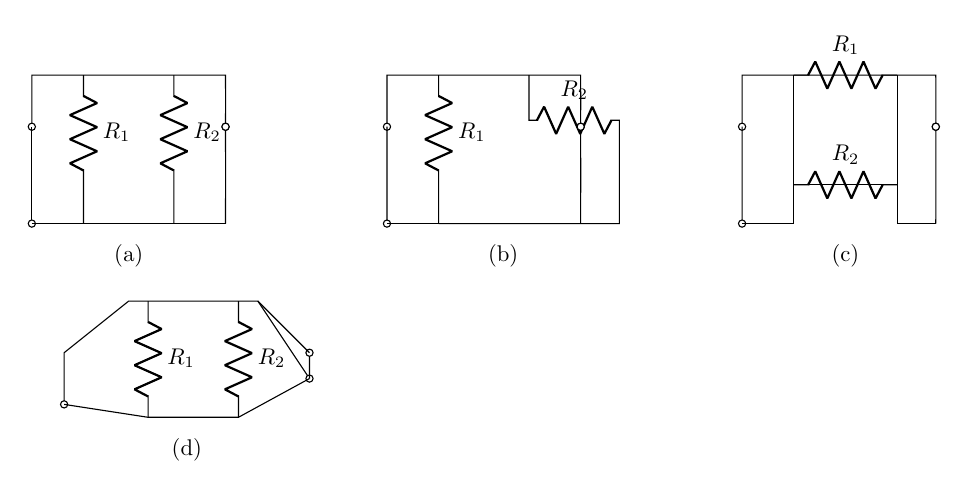
\begin{tikzpicture}[scale=0.82, transform shape]
  % drawing 1
  \draw (0,4.5) to[short,o-] (0,5.3) -- (3,5.3) to[short,-o] (3,4.5);
  \draw (0.8,5.3) to[R=$R_1$] (0.8,3.5) -- (0.8,3.0);
  \draw (2.2,5.3) to[R=$R_2$] (2.2,3.5) -- (2.2,3.0);
  \draw (0.8,3.0) -- (2.2,3.0);
  \draw (0,3.0) to[short,o-] (0,4.5); \draw (3,3.0) to[short,-o] (3,4.5);
  \draw (0,3.0) -- (0.8,3.0); \draw (2.2,3.0) -- (3,3.0);
  \node[below] at (1.5,2.8) {(a)};
  % drawing 2: folded rail
  \draw (5.5,4.5) to[short,o-] (5.5,5.3) -- (8.5,5.3) to[short,-o] (8.5,4.5);
  \draw (6.3,5.3) to[R=$R_1$] (6.3,3.5) -- (6.3,3.0);
  \draw (7.7,5.3) -- (7.7,4.6) to[R=$R_2$] (9.1,4.6) -- (9.1,3.0) -- (6.3,3.0);
  \draw (5.5,3.0) to[short,o-] (5.5,4.5); \draw (8.5,3.0) to[short,-o] (8.5,4.5);
  \draw (5.5,3.0) -- (6.3,3.0); \draw (8.5,3.0) -- (8.5,3.0);
  \node[below] at (7.3,2.8) {(b)};
  % drawing 3: sideways
  \draw (11,4.5) to[short,o-] (11,5.3) -- (14,5.3) to[short,-o] (14,4.5);
  \draw (11.8,5.3) to[R=$R_1$] (13.4,5.3);
  \draw (11.8,3.6) to[R=$R_2$] (13.4,3.6);
  \draw (11.8,3.0) -- (11.8,5.3); \draw (13.4,3.0) -- (13.4,5.3);
  \draw (11.8,3.6) -- (13.4,3.6);
  \draw (11,3.0) to[short,o-] (11,4.5); \draw (14,3.0) to[short,-o] (14,4.5);
  \draw (11,3.0) -- (11.8,3.0); \draw (13.4,3.0) -- (14,3.0);
  \node[below] at (12.6,2.8) {(c)};
  % drawing 4: squashed triangle
  \draw (0.5,0.2) to[short,o-] (0.5,1.0) -- (1.5,1.8) -- (3.5,1.8) to[short,-o] (4.3,0.6);
  \draw (1.8,1.8) to[R=$R_1$] (1.8,0.0);
  \draw (3.2,1.8) to[R=$R_2$] (3.2,0.0);
  \draw (0.5,0.2) -- (1.8,0.0) -- (3.2,0.0) -- (4.3,0.6);
  \draw (4.3,0.6) to[short,-o] (4.3,1.0); \draw (4.3,1.0) -- (3.5,1.8);
  \node[below] at (2.4,-0.2) {(d)};
\end{tikzpicture}

\caption{One parallel circuit, four drawings. In every panel each end of
$R_1$ shares a node with an end of $R_2$ and nothing in between splits them.
If you can label only two distinct nodes, the resistors are in parallel —
however the wires are bent.}
\label{fig:redraws}
\end{figure}

\begin{exercise}[easy]
In Figure~\ref{fig:redraws}(b), trace from the top of $R_1$ to the top of
$R_2$ without lifting your pen. You never pass through a component — so those
ends are one node. Do the same for the bottoms.
\end{exercise}

\section{Equivalent resistance}
\label{sec:req}

A network of resistors between two terminals behaves, at those terminals, like
one resistor called the \emph{equivalent resistance}\index{equivalent
resistance} $R_{\mathrm{eq}}$. Two cases cover nearly everything.

\textbf{Series:} the same current crosses both, voltages add (KVL), so
$R_{\mathrm{eq}} = R_1 + R_2$. \textbf{Parallel:} the same voltage sits across
both, currents add (KCL):
\[
\frac{1}{R_{\mathrm{eq}}} = \frac{1}{R_1} + \frac{1}{R_2}
\qquad\Longleftrightarrow\qquad
R_{\mathrm{eq}} = \frac{R_1 R_2}{R_1 + R_2}\quad\text{("product over sum")}.
\]
For $n$ resistors, series just sums; parallel sums the reciprocals. Reduce
any network by repeatedly collapsing the two-terminal pieces. Sanity checks
that catch almost every slip: in parallel, $R_{\mathrm{eq}}$ is
\emph{smaller than the smallest} resistor (more paths, more current); in
series, $R_{\mathrm{eq}}$ is larger than the largest.

\begin{exercise}[easy]
Reduce this to one resistor: \qty{1}{\kilo\ohm} in parallel with
\qty{2}{\kilo\ohm}, in series with \qty{470}{\ohm}. (Answer:
$667 + 470 \approx \qty{1.14}{\kilo\ohm}$.)
\end{exercise}

\section{The voltage divider}
\label{sec:divider}

Two series resistors across a source split the voltage in proportion to their
resistances. With $R_1$ on top and $R_2$ to ground as in
Figure~\ref{fig:divider},
\[
v_{\mathrm{out}} \;=\; V_{\mathrm{in}}\,\frac{R_2}{R_1+R_2}.
\]
One line of KVL derives it: the current is $V_{\mathrm{in}}/(R_1+R_2)$, and
the output is that current times $R_2$. This fragment appears dozens of times
in this book — scaling sensor signals, setting logic levels, biasing
transistors. Learn it once, recognise it everywhere.

\begin{figure}[htbp]
\centering
% fig_divider.tex -- Figure 3.2: annotated voltage divider
\begin{circuitikz}[american]
  \draw (0,0) to[battery1, l_=$V_{\mathrm{in}}$, invert] (0,4);
  \draw (0,4) to[R, l=$R_1$, v^>=$v_{R1}$, i>_=$i$] (3,4);
  \draw (3,4) to[R, l=$R_2$, v^>=$v_{\mathrm{out}}$, i>_=$i$] (3,0) -- (0,0);
  \draw (3,4) to[short,-o] (4.3,4) node[right]{$v_{\mathrm{out}}$};
  \node[right,align=left] at (4.8,2.6) {$v_{\mathrm{out}} = V_{\mathrm{in}}\,\dfrac{R_2}{R_1+R_2}$\\[4pt] $i = \dfrac{V_{\mathrm{in}}}{R_1+R_2}$};
\end{circuitikz}

\caption{The voltage divider. The output is taken \emph{at the middle node};
$R_2$ is the resistor \emph{to ground}. Notice the formula needs the same
current through both — the moment something draws current out of the middle
node, $v_{\mathrm{out}}$ falls (Section~\ref{sec:thevenin} quantifies it).}
\label{fig:divider}
\end{figure}

\begin{example}[A 3.3 V logic level from a 5 V rail]
\label{ex:div33}
\textbf{Strategy.} The ratio sets the voltage; the absolute values set how
much current the divider wastes. Pick a ratio from the E24 ladder, then
choose a magnitude that burns little current but still makes the output
stiff compared to anything the logic input draws (chip inputs want microamps
or less).

\textbf{Solution.} We need $R_2/(R_1+R_2) = 3.3/5 = 0.66$, i.e.
$R_1 : R_2 \approx 1 : 1.94$. E24 gives a clean hit: $R_1=\qty{1}{\kilo\ohm}$,
$R_2=\qty{2}{\kilo\ohm}$, ratio $2000/3000=0.667$.
Then $v_{\mathrm{out}}=5\times0.667=\qty{3.33}{\volt}$ and the standing
current is $5/3000=\qty{1.67}{\milli\ampere}$ — under \qty{10}{\milli\watt}
from the rail. Tolerance corners (\qty{5}{\percent} parts): worst high is
$5\times2.1/3.05=\qty{3.44}{\volt}$, worst low is
$5\times1.9/2.95=\qty{3.22}{\volt}$ — a \qty{3.3}{\volt} input typically
accepts down to about \qty{2.5}{\volt} as "high", so both corners pass.

\textbf{Check.} Listing~\ref{lst:dividerop} runs it. Notice the simulator
takes the question "what are all node voltages and branch currents" literally
— and answers 3.33 V and $1.67$ mA exactly as derived.
\end{example}

\begin{lstlisting}[language={},caption={\texttt{code/ch03\_divider.cir} — the divider as a netlist.},label=lst:dividercir]
* ch03_divider.cir -- 5 V -> 3.3 V divider, operating point
V1 1 0 DC 5
R1 1 2 1000
R2 2 0 2000
.op
.end
\end{lstlisting}

\begin{lstlisting}[language={},caption={ngspice output of \texttt{code/ch03\_divider.cir}, verbatim (simulation S1).},label=lst:dividerop]
V(2)                             3.333333e+00
V(1)                             5.000000e+00
v1#branch                        -1.66667e-03
\end{lstlisting}

\section{The current divider}
\label{sec:curdiv}

Parallel is the mirror image. Two parallel resistors share a voltage and split
an incoming current \emph{inversely} to their resistances — more current takes
the easier path:
\[
i_2 = I\,\frac{R_1}{R_1+R_2}.
\]
Note the twist: the current through $R_2$ is proportional to the
\emph{other} resistor. (The clean derivation uses conductances
$G=1/R$\index{conductance}: in parallel, conductances add and current splits
in proportion to $G$, i.e. $i_2 = I\,G_2/(G_1+G_2)$ — same thing, one less
fraction to fumble.)

\section{KCL and KVL: bookkeeping, signed}
\label{sec:klaws}

\begin{definition}[Kirchhoff's current law]\index{Kirchhoff's current law}
The sum of currents \emph{into} a node is zero — or equivalently, what flows
in flows out. Charge is conserved and nodes store none of it.
\end{definition}

\begin{definition}[Kirchhoff's voltage law]\index{Kirchhoff's voltage law}
The sum of signed voltage changes around any closed loop is zero. Voltage is
a potential difference; returning to the same node must return the same
potential.
\end{definition}

The laws are trivial. The discipline is the \emph{signs}. Pick a direction and
label every drop before writing equations — Figure~\ref{fig:kvlkcl} marks the
convention this book uses: a drop is $+$ when your loop direction enters the
$+$ labelled terminal. Then the equation writes itself. Sign errors, not
concept errors, are what actually go wrong (Section~\ref{sec:mistakes3}).

\begin{figure}[htbp]
\centering
% fig_kvlkcl.tex -- Figure 3.3: KVL signed drops + KCL node
\begin{circuitikz}[american]
  % left: KVL loop
  \draw (0,0) to[battery1, l_=\qty{9}{\volt}, invert] (0,3.4);
  \draw (0,3.4) to[R, l=\qty{220}{\ohm}, v^<=$v_1$] (3,3.4);
  \draw (3,3.4) to[R, l=\qty{470}{\ohm}, v^<=$v_2$] (3,0) -- (0,0);
  \draw[->,thick] (0.9,1.2) arc[start angle=200,end angle=-20,radius=0.75];
  \node at (1.55,1.5) {$\sum v_k = 0$};
  % right: KCL node
  \node[circ] (n) at (7,2.2) {};
  \draw (n) -- (5.4,3.4) node[left]{$i_1$};
  \draw (n) -- (8.6,3.4) node[right]{$i_2$};
  \draw (n) -- (7,0.8) node[below]{$i_3$};
  \draw[->,thick] (5.9,3.2) -- (6.8,2.4);
  \draw[->,thick] (8.1,3.2) -- (7.2,2.4);
  \draw[->,thick] (7,1.6) -- (7,2.0);
  \node[right,align=left] at (8.8,1.6) {signs first:\\ $+i_1+i_2-i_3=0$\\ if $i_3$ leaves};
  \node[below] at (9.6,0.6) {};
\end{circuitikz}

\caption{Left: KVL on the series loop — walking clockwise,
$+9 - v_1 - v_2 = 0$. Right: KCL at a node — assign each current a direction
\emph{first} (here $i_3$ defined leaving), then sum algebraically:
$i_1 + i_2 - i_3 = 0$. Negative answers just mean "the arrow was guessed
backwards", which is fine.}
\label{fig:kvlkcl}
\end{figure}

\begin{checkpoint}
In Figure~\ref{fig:kvlkcl} (left), $v_1=\qty{3}{\volt}$. Write the KVL sum
and find $v_2$ without computing any current. (Answer:
$9-3-v_2=0 \Rightarrow v_2=\qty{6}{\volt}$.)
\end{checkpoint}

\section{The node-voltage method}
\label{sec:nodevoltage}

For a network that will not collapse to one $R_{\mathrm{eq}}$, do this
instead\index{node-voltage method}: pick a ground, name every other node
voltage $v_1, v_2, \dots$, and write KCL at each node with each current
expressed via Ohm's law. One equation per node, solved together — that is the
entire method, and it is exactly what the simulator does internally.

\begin{example}[Two sources, one node: by hand then by ngspice]
\label{ex:twoloop}
\textbf{Strategy.} Node 3 joins three resistors to two sources. Write KCL
there; the branch currents are $(v_3 - 12)/100$, $(v_3 - 6)/220$ and
$v_3/470$. One unknown, one equation.

\textbf{Solution.}
\[
\frac{v_3-12}{100} + \frac{v_3-6}{220} + \frac{v_3}{470} = 0
\;\Longrightarrow\;
v_3\!\left(\tfrac{1}{100}+\tfrac{1}{220}+\tfrac{1}{470}\right)
= \tfrac{12}{100}+\tfrac{6}{220}
\]
\[
v_3 = \frac{0.1473}{0.01667} \approx \qty{8.83}{\volt}.
\]
Notice the form: \emph{weighted average}. $v_3$ lies between 6 and 12 V,
pulled toward the 12 V source because its \qty{100}{\ohm} link is the
strongest (lowest resistance).

\textbf{Check.} Listing~\ref{lst:twoloopop} — ngspice agrees to the fourth
decimal, and reports the branch currents $-31.7$ mA and $+12.9$ mA that the
hand work predicts ($\frac{8.83-12}{100}=-31.7$ mA;
$\frac{8.83-6}{220}=+12.9$ mA; both plus $v_3/470=18.8$ mA sum to zero —
KCL, closing the loop on itself).
\end{example}

\begin{lstlisting}[language={},caption={\texttt{code/ch03\_twoloop.cir} — the two-source network of Example~\ref{ex:twoloop}.},label=lst:twoloopcir]
* ch03_twoloop.cir -- two sources feeding one node through resistors
V1 1 0 DC 12
V2 2 0 DC 6
R1 1 3 100
R2 2 3 220
R3 3 0 470
.op
.end
\end{lstlisting}

\begin{lstlisting}[language={},caption={ngspice output of \texttt{code/ch03\_twoloop.cir}, verbatim (simulation S2).},label=lst:twoloopop]
V(3)                             8.832947e+00
V(2)                             6.000000e+00
V(1)                             1.200000e+01
v1#branch                        -3.16705e-02
v2#branch                        1.287703e-02
\end{lstlisting}

\section{Th\'evenin and Norton: networks compressed}
\label{sec:thevenin}

\begin{definition}[Th\'evenin equivalent]\index{Th\'evenin equivalent}
Any linear network viewed from two terminals behaves exactly like one voltage
source $V_{\mathrm{th}}$ in series with one resistor $R_{\mathrm{th}}$:
$V_{\mathrm{th}}$ is the open-circuit voltage at the terminals, and
$R_{\mathrm{th}}$ is the resistance looking in (all independent sources
zeroed) — equivalently $R_{\mathrm{th}} = V_{\mathrm{th}}/I_{\mathrm{sc}}$
where $I_{\mathrm{sc}}$ is the short-circuit current.
\end{definition}

"Behaves exactly like" means \emph{for every possible load}: the terminal's
voltage-versus-load-current line is identical. Figure~\ref{fig:thevenin}
shows the picture; Figure~\ref{fig:loadline} proves it on the divider —
sweep a load current through the original and through the model and the lines
coincide. The \emph{Norton equivalent}\index{Norton equivalent} is the same
idea drawn the other way: a current source $I_{\mathrm{sc}}$ in parallel with
$R_{\mathrm{th}}$, interchangeable by $V_{\mathrm{th}}=I_{\mathrm{sc}}R_{\mathrm{th}}$.
Worked use of it: our divider's Norton form is \qty{5}{\milli\ampere} in
parallel with \qty{667}{\ohm}. Ask how much current a \qty{2}{\kilo\ohm} load
draws and the current divider answers in one line:
$5\,\mathrm{mA}\times 667/(667+2000) = \qty{1.25}{\milli\ampere}$ — the same
answer KCL gives on the full circuit ($v_{\mathrm{out}}=\qty{2.5}{\volt}$),
with the network replaced by two numbers. Norton is the natural form
whenever the quantity you care about is current — sensors, current-output
devices, parallel paths.

\begin{figure}[htbp]
\centering
% fig_thevenin.tex -- Figure 3.4: Thevenin equivalent picture
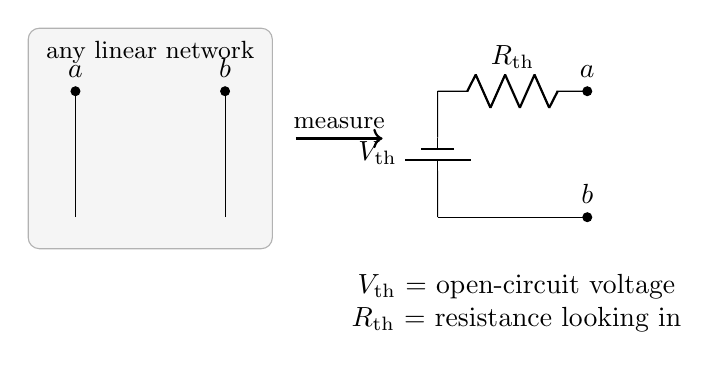
\begin{tikzpicture}
  % original network
  \draw[draw=gray!60,fill=gray!8,rounded corners] (-0.2,-0.4) rectangle (2.9,2.4);
  \node at (1.35,2.1) {\small any linear network};
  \draw (0.4,0) -- (0.4,1.6) node[circ,label=above:$a$]{};
  \draw (2.3,0) -- (2.3,1.6) node[circ,label=above:$b$]{};
  % arrow
  \draw[->,thick] (3.2,1.0) -- (4.3,1.0) node[midway,above]{\small measure};
  % thevenin
  \draw (5.0,1.6) to[battery1, l_=$V_{\mathrm{th}}$, invert] (5.0,0);
  \draw (5.0,1.6) to[R, l=$R_{\mathrm{th}}$] (6.9,1.6) node[circ,label=above:$a$]{};
  \draw (6.9,0) node[circ,label=above:$b$]{} -- (5.0,0);
  \node[below,align=center] at (6.0,-0.6) {$V_{\mathrm{th}}$ = open-circuit voltage\\ $R_{\mathrm{th}}$ = resistance looking in};
\end{tikzpicture}

\caption{The Th\'evenin picture: whatever is inside the left box — any number
of sources and resistors — the terminals see only $V_{\mathrm{th}}$ and
$R_{\mathrm{th}}$. Two measurements determine it: open-circuit voltage, and
either short-circuit current or resistance-with-sources-zeroed.}
\label{fig:thevenin}
\end{figure}

\begin{example}[The divider, compressed — and when "3.3 V" lies]
\label{ex:thevdiv}
\textbf{Strategy.} Compress the Example~\ref{ex:div33} divider
($R_1=\qty{1}{\kilo\ohm}$, $R_2=\qty{2}{\kilo\ohm}$ on 5 V) into a
Th\'evenin model, then ask it a loaded question.

\textbf{Solution.} $V_{\mathrm{th}}$ = open-circuit output = \qty{3.33}{\volt}.
Looking in with the 5 V source zeroed (shorted): $R_1$ and $R_2$ are both
from the output node to ground $\Rightarrow
R_{\mathrm{th}} = 1\|2\,\mathrm{k}\Omega = \qty{667}{\ohm}$.
Now attach a \qty{1}{\kilo\ohm} load: the model predicts
$v_{\mathrm{out}} = 3.33 \times 1000/1667 = \qty{2.0}{\volt}$ — the "3.3 V
rail" collapsed by \qty{40}{\percent}. The simplification does not lie; the
lie was treating an unstiff divider as a voltage source. The load-line
sweep in Figure~\ref{fig:loadline} (from the Listings below) shows the model
and the original agreeing to seven digits: slope $-667\ \Omega$, intercept
\qty{3.33}{\volt}, zero crossing at $I_{\mathrm{sc}}=\qty{5}{\milli\ampere}
= 3.33/0.667$.

\textbf{Rule of thumb.} A divider feeding a load wants
$R_{\mathrm{th}} \ll R_{\mathrm{load}}$ — a factor of 10 keeps the sag under
about \qty{9}{\percent}.
\end{example}

\begin{lstlisting}[language={},caption={\texttt{code/ch03\_thevenin.cir} — sweep a load current, record $v_{\mathrm{out}}$ (simulation S3). \texttt{code/ch03\_thevenin\_model.cir} is the same file with the two resistors replaced by $V_{\mathrm{th}}{=}\qty{3.333}{\volt}$ and $R_{\mathrm{th}}{=}\qty{667}{\ohm}$.},label=lst:thevcir]
* ch03_thevenin.cir -- load-line sweep: original divider
I1 2 0 DC 0          * load current pulled OUT of node 2
V1 1 0 DC 5
R1 1 2 1000
R2 2 0 2000
.control
dc i1 0 0.01 0.0005
let vout = v(2)
set filetype=ascii
wrdata ch03_divider_loadline.dat vout
.endc
.end
\end{lstlisting}

\begin{lstlisting}[language={},caption={Verification output, verbatim — every 4th row shown of 21 simulated rows: load current, $v_{\mathrm{out}}$ of the real divider, $v_{\mathrm{out}}$ of the Th\'evenin model. Column 3 minus column 2 never exceeds \qty{7e-8}{\volt} on any row.},label=lst:thevout]
i_load          v_orig          v_model
0.00000000e+00  3.33333333e+00  3.33333330e+00
2.00000000e-03  2.00000000e+00  1.99999996e+00
4.00000000e-03  6.66666667e-01  6.66666620e-01
6.00000000e-03 -6.66666667e-01 -6.66666720e-01
8.00000000e-03 -2.00000000e+00 -2.00000006e+00
1.00000000e-02 -3.33333333e+00 -3.33333340e+00
\end{lstlisting}

\begin{figure}[htbp]
\centering
% fig_loadline.tex -- Figure 3.6: load-line sweep, divider vs Thevenin model
\begin{tikzpicture}
\begin{axis}[width=0.85\textwidth, height=6.2cm,
  xlabel={load current (\unit{\milli\ampere})},
  ylabel={$v_{\mathrm{out}}$ (\unit{\volt})},
  xmin=0, xmax=10, ymin=0, ymax=3.6,
  grid=both, grid style={gray!15},
  legend style={at={(0.97,0.30)},anchor=east,font=\small}]
  \addplot[blue, thick] table[x index=0,y index=1,y expr={\thisrowno{0}*1}] {figures/ch03/ch03_loadline.dat};
  \addlegendentry{original divider}
  \addplot[red, dashed, thick] table[x index=0,y index=1] {figures/ch03/ch03_loadline_model.dat};
  \addlegendentry{Th\'evenin model}
  \addplot[black, only marks, mark=x, mark size=3pt] coordinates {(0,3.333) (5,0)};
  \node[font=\small, anchor=west] at (axis cs:0.25,3.42) {$V_{\mathrm{th}}=\qty{3.33}{\volt}$};
  \node[font=\small, anchor=south west] at (axis cs:5.15,0.02) {$I_{\mathrm{sc}}=\qty{5.0}{\milli\ampere}$};
\end{axis}
\end{tikzpicture}

\caption{Simulation S3: $v_{\mathrm{out}}$ against pulled load current for the
real divider (blue) and its Th\'evenin model (red, dashed) — the same line,
to \qty{70}{\nano\volt}. The marked endpoints are the theorem's two handles:
open-circuit voltage \qty{3.33}{\volt} and short-circuit current
\qty{5}{\milli\ampere}. Every linear network has exactly one such line.}
\label{fig:loadline}
\end{figure}

\section{Measuring without breaking the circuit}
\label{sec:meterloading}

A voltmeter connects in parallel — so it adds a resistance in parallel.
Real DMMs present about \qty{10}{\mega\ohm}\index{meter loading}; on
kiloohm-scale circuits that is invisible, but measure a megaohm divider and
the meter \emph{becomes part of the circuit}
(Figure~\ref{fig:meter}): $1\,\mathrm{M}\Omega \| 10\,\mathrm{M}\Omega =
\qty{909}{\kilo\ohm}$, so a \qty{5}{\volt} rail reads $5\times909/1909 =
\qty{2.38}{\volt}$ instead of \qty{2.5}{\volt}. The meter did not "use up"
voltage; it changed the divider. When a reading surprises you, suspect the
probe before the circuit.

\begin{figure}[htbp]
\centering
% fig_meter.tex -- Figure 3.5: meter loading
\begin{circuitikz}[american]
  \draw (0,0) to[battery1, l_=\qty{5}{\volt}, invert] (0,3.4);
  \draw (0,3.4) to[R, l=\qty{1}{\mega\ohm}] (3,3.4);
  \draw (3,3.4) to[R, l_=\qty{1}{\mega\ohm}] (3,0) -- (0,0);
  % DMM across bottom resistor
  \draw (3,3.4) -- (5,3.4) to[vR, l_=DMM, n=mymeter] (5,0) -- (3,0);
  \draw[dashed] (5,3.4) to[R, l=\qty{10}{\mega\ohm}] (5,0);
  \node[right,align=left] at (5.9,1.9) {reads \qty{2.38}{\volt},\\ not \qty{2.5}{\volt}};
\end{circuitikz}

\caption{Meter loading. Two \qty{1}{\mega\ohm} resistors divide 5 V to
\qty{2.5}{\volt} until a \qty{10}{\mega\ohm} meter joins the bottom leg —
\qty{2.38}{\volt} now. Dashed: the resistance you added by measuring.}
\label{fig:meter}
\end{figure}

\begin{exercise}[medium — predict, then run]
A \qty{4.7}{\mega\ohm} / \qty{4.7}{\mega\ohm} divider sits on \qty{9}{\volt}.
Predict the DMM reading ($R_{\mathrm{meter}}=\qty{10}{\mega\ohm}$), write the
three-line netlist, run it, compare. (Answer: $4.7\|10=\qty{3.20}{\mega\ohm}$,
$9\times3.20/7.90=\qty{3.64}{\volt}$ — the meter drags it down by
\qty{19}{\percent}.)
\end{exercise}

\section{Common mistakes}
\label{sec:mistakes3}

\begin{tripwire}[KVL around a non-loop / KCL at a non-node]
Writing $\sum v = 0$ across elements that do not form a closed loop, or
summing currents at a "node" that secretly contains a junction you missed.
Trace the loop with a finger; list the node's wires explicitly.
\end{tripwire}

\begin{tripwire}[Signs guessed mid-equation]
Assigning polarities while solving instead of before. If $v_1$ was labelled
one way in the figure and flipped in the algebra, the sign error compounds
silently. Label first; solve second; never adjust.
\end{tripwire}

\begin{tripwire}[Using the divider formula on a loaded divider]
$v_{\mathrm{out}} = V R_2/(R_1+R_2)$ assumes the middle node's only currents
are through $R_1$ and $R_2$. Any load at the node breaks the premise —
Example~\ref{ex:thevdiv}'s \qty{2.0}{\volt} instead of \qty{3.3}{\volt}.
Check what else connects.
\end{tripwire}

\begin{tripwire}[Mixing series and parallel formulas mid-redraw]
$R_1+R_2$ used where resistors share a node-pair but also a third element,
or "product over sum" applied to resistors that are not both on the same two
nodes. Redraw to the canonical form of Figure~\ref{fig:redraws} before any
arithmetic.
\end{tripwire}

\section{Chapter summary}
\label{sec:ch3summary}

Figure~\ref{fig:cheatsheet} is the whole chapter on one card. The method
hierarchy: redraw until it is series/parallel; if it will not collapse, write
KCL at each node; if you only care about one port, compress to Th\'evenin.
Everything else is algebra.

\begin{figure}[htbp]
\centering
% fig_cheatsheet.tex -- Figure 3.7: chapter cheat-sheet table (used as summary)
\begin{tabular}{@{}llll@{}}
\toprule
Quantity & Series & Parallel & Note \\
\midrule
Resistance & $R_{\mathrm{eq}}=R_1+R_2$ & $R_{\mathrm{eq}}=\dfrac{R_1R_2}{R_1+R_2}$ & two at a time \\
Voltage & splits $\propto R$ & same on each & KVL \\
Current & same through each & splits $\propto 1/R$ & KCL \\
Divider & $v_{\mathrm{out}}=V\dfrac{R_2}{R_1+R_2}$ & $i_2=I\dfrac{R_1}{R_1+R_2}$ & unloaded! \\
Th\'evenin & $V_{\mathrm{th}}=v_{\mathrm{oc}}$ & $R_{\mathrm{th}}=V_{\mathrm{th}}/I_{\mathrm{sc}}$ & one line fits all loads \\
\bottomrule
\end{tabular}

\caption{Cheat-sheet for Chapter 3. The last row is why Th\'evenin matters:
one measured line replaces the whole internal network.}
\label{fig:cheatsheet}
\end{figure}

\begin{wins}
\begin{itemize}
\item You classify connections by node counting and reduce any
series/parallel network to one resistor.
\item You can design and load-check a voltage divider — the most common two
resistors in this book.
\item KCL, KVL and the node-voltage method solve any linear resistive
circuit; you verified one against ngspice to the fourth decimal.
\item Th\'evenin compression tells you when a "supply" will sag, and the
meter-loading rule keeps your measurements honest.
\end{itemize}
\end{wins}

\section*{Exercises}
\addcontentsline{toc}{section}{Exercises}

\begin{exercise}[easy]
Three resistors — \qty{1}{\kilo\ohm}, \qty{2}{\kilo\ohm}, \qty{3}{\kilo\ohm} —
are placed end-to-end in a ring, terminals taken across the
\qty{1}{\kilo\ohm} only. What is $R_{\mathrm{eq}}$? (Careful: it is a
parallel question.)
\end{exercise}

\begin{exercise}[easy]
A node has four wires carrying \qty{2}{\milli\ampere},
\qty{-5}{\milli\ampere} and \qty{4}{\milli\ampere} (signs = into node).
What does the fourth carry?
\end{exercise}

\begin{exercise}[easy]
Using Figure~\ref{fig:divider}'s labels: $V_{\mathrm{in}}=\qty{12}{\volt}$,
$R_1=\qty{4.7}{\kilo\ohm}$, $R_2=\qty{10}{\kilo\ohm}$. Find
$v_{\mathrm{out}}$ and the standing current.
\end{exercise}

\begin{exercise}[easy]
True or false, with a one-sentence justification: two \qty{100}{\ohm}
resistors in parallel carry the same current as one \qty{50}{\ohm} resistor
at the same voltage.
\end{exercise}

\begin{exercise}[medium — derive]
Derive the parallel law from KCL: for $n$ resistors on the same node pair at
voltage $v$, show $1/R_{\mathrm{eq}} = \sum 1/R_k$; specialise to the
product-over-sum two-resistor form.
\end{exercise}

\begin{exercise}[medium — the classic trap]
Design a divider that outputs \qty{3.3}{\volt} from \qty{5}{\volt}
\emph{while the output node sources \qty{10}{\milli\ampere}}. Hint: you
cannot treat the load as infinite — write KCL at the output node including
the \qty{10}{\milli\ampere}. Choose real E24 values and report the delivered
voltage.
\end{exercise}

\begin{exercise}[medium]
Find the Th\'evenin equivalent of: \qty{9}{\volt} source, \qty{2}{\kilo\ohm}
series, \qty{3}{\kilo\ohm} to ground, terminals at the middle node. Then
predict the terminal voltage with a \qty{6}{\kilo\ohm} load.
\end{exercise}

\begin{exercise}[medium]
You probe the middle of an unloaded \qty{100}{\kilo\ohm}/\qty{100}{\kilo\ohm}
divider on \qty{10}{\volt} and read \qty{4.762}{\volt}. Infer the meter's
input resistance.
\end{exercise}

\begin{exercise}[hard — mesh]
The circuit of Example~\ref{ex:twoloop} modified: add a fourth resistor
\qty{330}{\ohm} from node 3 to a \emph{new} node 4, and connect node 4 to
ground through \qty{680}{\ohm}. Write the two node-voltage equations, solve
by hand, then confirm with a netlist you write yourself.
\end{exercise}

\begin{exercise}[hard]
A linear network is characterised only by two measurements: open-circuit
\qty{4.2}{\volt}; with a \qty{1}{\kilo\ohm} load it reads \qty{3.0}{\volt}.
Reconstruct $V_{\mathrm{th}}$ and $R_{\mathrm{th}}$, and state what load
resistance would pull the terminal down to half its open-circuit value.
\end{exercise}

\section*{Hints and answers}
\addcontentsline{toc}{section}{Hints and answers}

\begin{description}
\item[Ring.] \qty{1}{\kilo\ohm} in parallel with the series chain
$(2+3)\,\mathrm{k}\Omega$: $R_{\mathrm{eq}}=1000\cdot5000/6000
\approx\qty{833}{\ohm}$.
\item[KCL.] The three given sum to $+1$ mA; the fourth must carry
\qty{-1}{\milli\ampere} (i.e.\ \qty{1}{\milli\ampere} leaving).
\item[12 V divider.] $v_{\mathrm{out}}=12\times10/14.7=\qty{8.16}{\volt}$;
$i=12/14.7\,\mathrm{k}=\qty{0.816}{\milli\ampere}$.
\item[50 ohm.] True — equivalence means identical terminal behaviour; that is
the definition's whole point.
\item[Derivation.] Same $v$ on all $n$ branches, $i_k=v/R_k$, KCL gives
$I=v\sum 1/R_k$; compare with $I=v/R_{\mathrm{eq}}$. For $n=2$:
$R_{\mathrm{eq}}=1/(1/R_1+1/R_2)=R_1R_2/(R_1+R_2)$.
\item[Loaded divider.] KCL at the output: $(5-v)/R_1 = v/R_2 + 0.01$ with
$v=3.3$. Pick $R_1=\qty{100}{\ohm}$: $17$ mA in, so $3.3/R_2=7$ mA,
$R_2\approx\qty{471}{\ohm}\to\qty{470}{\ohm}$ E24; simulated value
$\approx\qty{3.30}{\volt}$. Any pair with the same current budget works.
\item[Th\'evenin.] $V_{\mathrm{th}}=9\times3/5=\qty{5.4}{\volt}$;
$R_{\mathrm{th}}=2\|3=\qty{1.2}{\kilo\ohm}$; loaded:
$5.4\times6/7.2=\qty{4.5}{\volt}$.
\item[Meter inference.] Reading $4.762=10\times R_{\mathrm{eq}}/(100+R_{\mathrm{eq}})$
gives $R_{\mathrm{eq}}\approx\qty{90.9}{\kilo\ohm}$, so
$R_{\mathrm{meter}}\approx\qty{1}{\mega\ohm}$.
\item[Mesh/nodes.] Equations: $(v_3-12)/100+(v_3-6)/220+v_3/470+(v_3-v_4)/330=0$;
$v_4/680+(v_4-v_3)/330=0$. Second gives $v_4=0.673\,v_3$; substituting,
$v_3\approx\qty{8.34}{\volt}$, $v_4\approx\qty{5.61}{\volt}$.
\item[Two measurements.] $V_{\mathrm{th}}=\qty{4.2}{\volt}$; under
\qty{1}{\kilo\ohm}: $3.0=4.2\times1000/(R_{\mathrm{th}}+1000)$ gives
$R_{\mathrm{th}}=\qty{400}{\ohm}$; half open-circuit when
$R_{\mathrm{load}}=R_{\mathrm{th}}=\qty{400}{\ohm}$.
\end{description}

\chapternotes
\begin{enumerate}
\item Series/parallel-by-nodes presentation and the four-redraws exercise
format follow the sequencing of Kuphaldt's Vol.~I ch.~5--6 \cite{aacvol1};
the example networks are original constructions.
\item The node-voltage method and the weighted-average reading of
Example~\ref{ex:twoloop} track MIT 6.002 lectures 1--3 \cite{ocw6002}, which
also teach Th\'evenin as a load-line measurement — the basis of
Figure~\ref{fig:loadline}'s simulation.
\item Meter-loading numbers use the conventional \qty{10}{\mega\ohm} DMM
input resistance \cite{sparkfunmultimeter}.
\item All ngspice outputs in this chapter are verbatim from ngspice-47 on the
author's machine; the load-line agreement ($<\qty{1e-7}{\volt}$) is exact up
to the model's truncated $V_{\mathrm{th}}$ \cite{ngspice}.
\end{enumerate}

% ch04-electronics.tex -- Chapter 4: Capacitors, inductors and RC/RL transients
\chapter{Capacitors, inductors and RC/RL transients}
\label{ch:transients}

Chapters 1--3 lived in a world where every voltage settles instantly. Real
circuits don't: they have \emph{memory}, and the two components that carry it
are the capacitor and the inductor. This chapter gives you the one
differential equation this book needs, its famous answer (the exponential,
with time constant $\tau$), and the three places transients actually ambush
you on a bench: switch debouncing, power-up behaviour, and the decoupling
capacitor that guards every chip's supply pin. By the end you can predict a
delay to the millisecond, size an RC for it, simulate the response, and
explain why opening an inductor's circuit is a way to kill a transistor.

\section{The capacitor: charge bucket, $i = C\,dv/dt$}
\label{sec:cap}

A \emph{capacitor}\index{capacitor} is two conductors facing each other
across an insulator. Charge pushed onto one plate repels charge off the
other; the stored charge is $Q = CV$, where the \emph{capacitance}
\index{capacitance} $C$ in farads measures how much charge one volt packs
away. Since current is charge per second, differentiating gives the element
law:
\[
i = C\,\frac{dv}{dt}.
\]
Read it both ways: current \emph{through} a capacitor means its voltage is
\emph{changing}, and a capacitor whose voltage is changing draws or supplies
current proportional to the rate. Two consequences worth memorising now:
capacitor voltage \emph{cannot jump} (a jump would need infinite current),
and at DC a charged capacitor is an open circuit — zero $dv/dt$, zero current.

\begin{figure}[htbp]
\centering
% fig_charge.tex -- Figure 4.1: capacitor as charge bucket
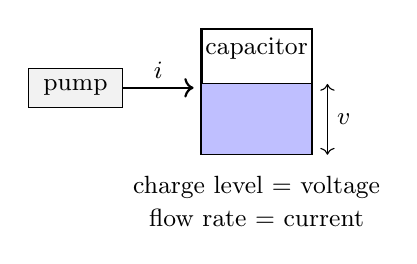
\begin{tikzpicture}
  % battery pumping charge
  \draw[fill=gray!10] (0,0) rectangle (1.2,0.5);
  \node at (0.6,0.25) {\small pump};
  \draw[->,thick] (1.2,0.25) -- (2.1,0.25);
  \node[above] at (1.65,0.25) {\small $i$};
  % bucket
  \draw[thick] (2.2,-0.6) -- (2.2,1.0) -- (3.6,1.0) -- (3.6,-0.6);
  \draw[fill=blue!25] (2.2,-0.6) rectangle (3.6,0.3);
  \draw[<->] (3.8,-0.6) -- (3.8,0.3) node[midway,right]{\small $v$};
  \node at (2.9,0.75) {\small capacitor};
  \node[below,align=center] at (2.9,-0.75) {\small charge level = voltage\\ \small flow rate = current};
\end{tikzpicture}

\caption{The bucket picture. Charge is the water level (voltage), current is
the flow rate, capacitance is the bucket's width. A wide bucket ($C$ big)
fills slowly for the same flow — that is why big capacitors make slow
circuits.}
\label{fig:charge04}
\end{figure}

The stored energy is $E=\tfrac12 CV^2$ — real energy, returned later, which
is what makes capacitors useful for smoothing and why a charged capacitor on
an unplugged board still bites (Section~\ref{sec:safety4}).

\section{The RC step response}
\label{sec:rcstep}

Connect a resistor from a voltage source to an uncharged capacitor
(Figure~\ref{fig:divider} of Chapter~3, second element now a $C$). KCL at the
capacitor node:
\[
\frac{V-v}{R} = C\frac{dv}{dt}
\quad\Longrightarrow\quad
\frac{dv}{dt}+\frac{v}{RC}=\frac{V}{RC}.
\]
This is a first-order linear ODE — the only one this book asks you to derive,
once, in the exercises. Its solution for $v(0)=0$ is
\[
v(t) = V\bigl(1-e^{-t/\tau}\bigr),\qquad \tau = RC,
\]
where $\tau$\index{time constant} — the \emph{time constant} — is the single
number that controls everything. The derivation matters once; the shape
matters forever (Figure~\ref{fig:rcstep}).

\begin{figure}[htbp]
\centering
% fig_rcstep.tex -- Figure 4.2: RC step response, real .tran data
\begin{tikzpicture}
\begin{axis}[width=0.85\textwidth, height=6cm,
  xlabel={$t$ (\unit{\milli\second})}, ylabel={$v_C$ (\unit{\volt})},
  xmin=0, xmax=5, ymin=0, ymax=5.4, grid=both, grid style={gray!15}]
  \addplot[blue, thick] table {figures/ch04/ch04_rc_step_ms.dat};
  \addplot[gray, dashed] coordinates {(0,5) (5,5)};
  \node[font=\small] at (axis cs:3.6,4.55) {$v_C = 5(1-e^{-t/\tau})$};
\end{axis}
\end{tikzpicture}

\caption{Real \texttt{.tran} output of the RC step: \qty{5}{\volt} through
\qty{1}{\kilo\ohm} into \qty{1}{\micro\farad}, so $\tau=\qty{1}{\milli\second}$.
Notice the charging is fastest at the start — the gap between target and
present voltage is what drives the current, so the approach is always
exponential, never linear.}
\label{fig:rcstep}
\end{figure}

\begin{figure}[htbp]
\centering
% fig_tau.tex -- Figure 4.3: tau marked at 63%
\begin{tikzpicture}
\begin{axis}[width=0.85\textwidth, height=6cm,
  xlabel={$t$ (\unit{\milli\second})}, ylabel={$v_C$ (\unit{\volt})},
  xmin=0, xmax=5, ymin=0, ymax=5.4, grid=both, grid style={gray!15}]
  \addplot[blue, thick] table {figures/ch04/ch04_rc_step_ms.dat};
  \addplot[gray, dashed] coordinates {(0,3.162) (1,3.162) (1,0)};
  \addplot[black, only marks, mark=*, mark size=1.8pt] coordinates {(1,3.162)};
  \node[font=\small, anchor=west] at (axis cs:1.15,3.162) {\qty{63}{\percent} at $t=\tau$};
  \node[font=\small] at (axis cs:2.9,1.1) {each $\tau$ erases \qty{63}{\percent} of what is left};
  \addplot[gray, dotted] coordinates {(0,5) (5,5)};
\end{axis}
\end{tikzpicture}

\caption{The number to memorise: at $t=\tau$ the capacitor reaches
\qty{63}{\percent} ($1-e^{-1}$) of its target. Each further $\tau$ closes
\qty{63}{\percent} of the \emph{remaining} gap — at $5\tau$ it is
\qty{99.3}{\percent} there, which is the engineer's ``done''.}
\label{fig:tau}
\end{figure}

\begin{checkpoint}
The sim above uses $R=\qty{1}{\kilo\ohm}$, $C=\qty{1}{\micro\farad}$.
Predict $v_C$ at $t=\qty{2}{\milli\second}$: $5(1-e^{-2})=\qty{4.32}{\volt}$.
The simulation agrees to three figures.
\end{checkpoint}

\section{Charging vs discharging}
\label{sec:chargedis}

Discharge is the mirror image: a charged cap through a resistor to ground
obeys $RC\,dv/dt = -v$, giving $v(t)=V_0 e^{-t/\tau}$ — the same exponential
flipped (Figure~\ref{fig:chargedis}). Charging and discharging are one
phenomenon — exponential approach to a target; only the target differs.

\begin{figure}[htbp]
\centering
% fig_chargedischarge.tex -- Figure 4.4: charging vs discharging
\begin{tikzpicture}
\begin{axis}[width=0.85\textwidth, height=6cm,
  xlabel={$t$ (\unit{\milli\second})}, ylabel={$v_C$ (\unit{\volt})},
  xmin=0, xmax=5, ymin=0, ymax=5.4, grid=both, grid style={gray!15},
  legend style={at={(0.97,0.5)},anchor=east,font=\small}]
  \addplot[blue, thick] table {figures/ch04/ch04_rc_step_ms.dat};
  \addlegendentry{charging toward 5 V}
  \addplot[red, thick] table {figures/ch04/ch04_rc_discharge_ms.dat};
  \addlegendentry{discharging toward 0}
\end{axis}
\end{tikzpicture}

\caption{Same $R$, same $C$, opposite targets — real \texttt{.tran} for both.
Notice the curves are reflections: at $t=\tau$ the charging curve sits at
\qty{63}{\percent} of full and the discharging at \qty{37}{\percent}.}
\label{fig:chargedis}
\end{figure}

\begin{exercise}[easy]
A \qty{1}{\micro\farad} cap charges through \qty{2.2}{\kilo\ohm} toward
\qty{5}{\volt}. Give $\tau$, and the voltage at $t=\tau$ and $t=3\tau$.
(Answer: \qty{2.2}{\milli\second}; \qty{3.16}{\volt}; \qty{4.75}{\volt}.)
\end{exercise}

\begin{example}[A 555-style delay: how long to \qty{3.33}{\volt}?]
\label{ex:delay555}
\textbf{Strategy.} The 555 timer (Chapter~13 territory) trips when its RC
reaches $\tfrac23 V_{CC}$. So the delay question is: for $v(t)=5(1-e^{-t/\tau})$,
solve $v(t^*)=\qty{3.33}{\volt}$.

\textbf{Solution.} $1-e^{-t/\tau}=2/3 \Rightarrow e^{-t/\tau}=1/3
\Rightarrow t^*=\tau\ln 3=1.0986\,\tau$. With $\tau=\qty{1}{\milli\second}$:
$t^*=\qty{1.099}{\milli\second}$.

\textbf{Check.} The \texttt{.tran} data of Listing~\ref{lst:rcstep} crosses
\qty{3.33}{\volt} at \qty{1.10}{\milli\second} — agreement to the third
digit, which is all the precision an electrolytic capacitor deserves.
\end{example}

\begin{lstlisting}[language={},caption={\texttt{code/ch04\_rc\_step.cir} — the step that produces Figures~\ref{fig:rcstep}--\ref{fig:tau} (simulation S1). The discharge twin \texttt{code/ch04\_rc\_discharge.cir} is the same file with the source removed and \texttt{.ic v(2)=5}.},label=lst:rcstep]
* ch04_rc_step.cir -- RC step response: 0->5 V step through R=1k into C=1uF
V1 1 0 PULSE(0 5 0 1n 1n 1 1)
R1 1 2 1000
C1 2 0 1u
.control
tran 5u 5m
let vout = v(2)
set filetype=ascii
wrdata ch04_rc_step.dat vout
.endc
.end
\end{lstlisting}

\begin{lstlisting}[language={},caption={Actual rows of \texttt{ch04\_rc\_step\_ms.dat} (the ms-rescaled file of Figure~\ref{fig:tau}; ngspice's adaptive steps land on these timestamps, not round numbers) — \qty{3.158}{\volt} at \qty{0.999}{\milli\second} is the 63\% mark, and \qty{3.334}{\volt} at \qty{1.099}{\milli\second} is the $\tau\ln 3$ crossing of Example~\ref{ex:delay555}.},label=lst:rcdata]
t(ms)           v(2)
8.988090e-01    2.964732e+00
9.988090e-01    3.158414e+00
1.098809e+00    3.333664e+00
1.198809e+00    3.492237e+00
\end{lstlisting}

\section{The inductor: the dual element}
\label{sec:ind}

The \emph{inductor}\index{inductor} mirrors the capacitor: a coil that stores
energy in its magnetic field and obeys
\[
v = L\,\frac{di}{dt},
\]
dual to $i=C\,dv/dt$\index{inductance}. Its time constant in a resistor
network is $\tau=L/R$\index{time constant!RL} — current through an inductor
cannot jump, and at DC it is a short. We keep it lighter than the capacitor
because its role in this book is mostly a warning label — the next section
shows why.

\begin{exercise}[easy]
An RL circuit has $L=\qty{10}{\milli\henry}$ in series with
$R=\qty{100}{\ohm}$. What is $\tau$, and how long until the current reaches
\qty{95}{\percent} of its final value? (Answer: \qty{100}{\micro\second};
$3\tau=\qty{300}{\micro\second}$.)
\end{exercise}

\section{RL transients and the flyback spike}
\label{sec:flyback}

Energise a coil and its current ramps exponentially toward $V/R$. Now open
the switch mid-current. The inductor's rule is absolute: $di/dt$ stays
finite, so the current \emph{keeps flowing} — and with nowhere to go it
charges whatever stray capacitance exists until the voltage is large enough
to find a path. That voltage is the \emph{flyback spike}\index{flyback}.

\begin{example}[Relay coil opened at \qty{171}{\milli\ampere}]
\label{ex:flyback}
\textbf{Strategy.} Coil \qty{10}{\milli\henry} with \qty{70}{\ohm} winding
resistance on \qty{12}{\volt}: steady current $12/70=\qty{171}{\milli\ampere}$.
Open the switch; the current has only the \qty{100}{\pico\farad} of stray
wiring capacitance to flow into. Energy conservation estimates the peak:
$\tfrac12 Li^2 \approx \tfrac12 Cv^2 \Rightarrow
v_{\mathrm{peak}}\approx i\sqrt{L/C}$.

\textbf{Solution.} $v_{\mathrm{peak}}\approx
0.171\sqrt{10\,\mathrm{m}/100\,\mathrm{p}} = 0.171\times10^{4}
\approx \qty{1.7}{\kilo\volt}$.

\textbf{Check.} Simulation S3 (Listings~\ref{lst:flybackcir},
Figure~\ref{fig:flyback}) peaks at \qty{1646}{\volt} — \qty{96}{\percent} of
the ideal estimate, the rest eaten by the coil resistance. A real bench sees
this as a killed transistor or a switch contact arc; Chapter~5's flyback
diode is the fix.
\end{example}

\begin{lstlisting}[language={},caption={\texttt{code/ch04\_relay\_flyback.cir} — simulation S3. The warning comment in the file is the point of the exercise.},label=lst:flybackcir]
* ch04_relay_flyback.cir -- open a relay coil mid-current, watch the node fly
* WARNING: the spike this produces (~1.7 kV simulated) is what kills
* transistors. The fix is Chapter 5's flyback diode -- do NOT leave the
* inductor's current path open in real hardware. Simulation S3.
* Topology: 12 V -> Rcoil -> node 2 -> coil L -> node 3 -> switch -> gnd
V1 1 0 DC 12
Rcoil 1 2 70
L1 2 3 10m IC=0
S1 3 0 10 0 SW1
Cpar 3 0 100p
Vsw 10 0 PULSE(1 0 1m 1n 1n 1 1)
.model SW1 SW vt=0.5 vh=0.1 ron=1 roff=1e9
.control
tran 500n 1.06m uic
let vnode = v(3)
wrdata ch04_flyback.dat vnode
.endc
.end
\end{lstlisting}

\begin{figure}[htbp]
\centering
% fig_flyback.tex -- Figure 4.5: relay flyback, real .tran data
\begin{tikzpicture}
\begin{axis}[width=0.85\textwidth, height=6.5cm,
  xlabel={$t$ (\unit{\milli\second})}, ylabel={$v_{\mathrm{node}}$ (\unit{\volt})},
  xmin=0.99, xmax=1.03, ymin=-200, ymax=1900, grid=both, grid style={gray!15}]
  \addplot[red, thick] table {figures/ch04/ch04_flyback_ms.dat};
  \addplot[black, only marks, mark=x, mark size=2.5pt] coordinates {(1.0014,1646)};
  \node[font=\small, anchor=west, align=left] at (axis cs:0.992,1500) {peak \qty{1646}{\volt}\\ predicted \qty{1714}{\volt}};
  \node[font=\small, anchor=west] at (axis cs:0.992,850) {switch opens at \qty{1}{\milli\second}};
\end{axis}
\end{tikzpicture}

\caption{Real \texttt{.tran} output: node 3 sits near ground while the switch
conducts, then leaps to \qty{1646}{\volt} in about a microsecond when it
opens. The marked peak is the estimate of Example~\ref{ex:flyback} — within
\qty{4}{\percent}.}
\label{fig:flyback}
\end{figure}

\section{Where transients hide}
\label{sec:hiding}

Three everyday cases, one physics.

\textbf{Debounce.} A mechanical contact bounces for milliseconds; an RC
filter with $\tau$ of a few ms smooths it into one clean edge (used in
Chapter~9's buttons).

\textbf{Power-up reset.} Hold a reset pin low while the rail climbs through
an RC — instant power-on becomes a deliberate delay, which is why chips come
up sane.

\textbf{Decoupling.} Every chip's supply pin gets a \qty{100}{\nano\farad}
capacitor to ground. When the chip gulps current, the wire's own resistance
would let the rail sag; the local capacitor covers the gulp while the supply
catches up. Example~\ref{ex:decouple} makes it quantitative.

\begin{example}[What \qty{100}{\nano\farad} does to a \qty{200}{\nano\second}
gulp]
\label{ex:decouple}
\textbf{Strategy.} Model the supply path as \qty{5}{\volt} through
\qty{10}{\ohm} of wire and trace impedance; the chip draws a
\qty{50}{\milli\ampere} step for \qty{200}{\nano\second}. Without a cap the
rail falls by Ohm's law; with one, the cap supplies the step and loses only
$\Delta v = I\,\Delta t/C$.

\textbf{Solution.} No cap: $\Delta v=50\,\mathrm{mA}\times10\,\Omega
=\qty{0.50}{\volt}$ — a \qty{10}{\percent} sag, enough to corrupt logic.
With \qty{100}{\nano\farad}: $\Delta v=50\,\mathrm{m}\times200\,\mathrm{n}
/100\,\mathrm{n}=\qty{0.10}{\volt}$.

\textbf{Check.} Simulation S2 (Listing~\ref{lst:decouplecir},
Figure~\ref{fig:decouple}): measured dips \qty{0.50}{\volt} and
\qty{0.091}{\volt} — the \qty{10}{\percent} residual is edge-rate, not
arithmetic. Decoupling is why chips don't brown out on their own switching.
\end{example}

\begin{lstlisting}[language={},caption={\texttt{code/ch04\_decouple.cir} — the with-capacitor run; \texttt{ch04\_decouple\_nocap.cir} removes line 5 (simulation S2, both halves).},label=lst:decouplecir]
* ch04_decouple.cir -- rail droop under a 200 ns, 50 mA current step
V1 1 0 DC 5
R1 1 2 10
C1 2 0 100n
I1 2 0 PULSE(0 0.05 0.5u 1n 1n 0.2u 1)
.control
tran 1n 1.5u
let vrail = v(2)
set filetype=ascii
wrdata ch04_decouple_cap.dat vrail
.endc
.end
\end{lstlisting}

\begin{figure}[htbp]
\centering
% fig_decouple.tex -- Figure 4.6: decoupling before/after, real .tran data
\begin{tikzpicture}
\begin{axis}[width=0.85\textwidth, height=6cm,
  xlabel={$t$ (\unit{\micro\second})}, ylabel={rail voltage (\unit{\volt})},
  xmin=0.3, xmax=1.0, ymin=4.35, ymax=5.1, grid=both, grid style={gray!15},
  legend style={at={(0.5,-0.28)},anchor=north,font=\small}]
  \addplot[gray, thick] table {figures/ch04/ch04_decouple_nocap_us.dat};
  \addlegendentry{no capacitor: \qty{0.50}{\volt} dip}
  \addplot[blue, thick] table {figures/ch04/ch04_decouple_cap_us.dat};
  \addlegendentry{with \qty{100}{\nano\farad}: \qty{0.091}{\volt} dip}
\end{axis}
\end{tikzpicture}

\caption{Real \texttt{.tran} data, zoomed to the gulp. Grey: the rail dips
\qty{0.50}{\volt} bare. Blue: \qty{100}{\nano\farad} holds it to
\qty{0.091}{\volt}. The capacitor does not remove the droop — it covers the
time the supply needs to respond.}
\label{fig:decouple}
\end{figure}

\begin{lstlisting}[language={},caption={\texttt{code/ch04\_tran\_csv.py} — the data pipeline: ngspice writes seconds; this rescales to ms/us for the figures. Every curve in this chapter passes through it.},label=lst:trancsv]
rescale("ch04_rc_step.dat",      "../figures/ch04/ch04_rc_step_ms.dat", 1e3, 4)
rescale("ch04_rc_discharge.dat", "../figures/ch04/ch04_rc_discharge_ms.dat", 1e3, 4)
rescale("ch04_decouple_cap.dat", "../figures/ch04/ch04_decouple_cap_us.dat", 1e6, 3)
rescale("ch04_decouple_nocap.dat","../figures/ch04/ch04_decouple_nocap_us.dat", 1e6, 3)
rescale("ch04_flyback.dat",      "../figures/ch04/ch04_flyback_ms.dat", 1e3, 2)
\end{lstlisting}

\begin{exercise}[medium]
A chip gulps \qty{100}{\milli\ampere} for \qty{50}{\nano\second}. Its
\qty{100}{\nano\farad} decoupling cap covers the gulp. How far does the
local rail sag? (Answer: $\Delta v=I\Delta t/C=\qty{0.05}{\volt}$.)
\end{exercise}

\section{$\star$ Driven RLC: why things ring}
\label{sec:rlc}

Optional, on first reading. Put $L$ and $C$ in one loop and their energies
trade back and forth — the capacitor pushes current that the inductor refuses
to stop, overshooting the target and oscillating at
$\omega_0=1/\sqrt{LC}$\index{ringing}. Resistance bleeds the oscillation
(``damping''); light damping leaves the bell-ringing you saw in
Figure~\ref{fig:flyback}'s spike. That is the whole story: flyback spikes,
switching noise, and every ``why is my square wave wiggly'' are this
exchange, at different $LC$. Chapter~6 uses $\omega_0$; the exercise asks you
to estimate it.

\section{Safety notes}
\label{sec:safety4}

\begin{rulebox}[Capacitors keep their charge]
A capacitor stores energy \emph{after} the power is off. Big electrolytics
can hold a painful voltage for hours — on any board, discharge large caps
through a resistor before touching. This book stays under \qty{9}{\volt}, but
the habit transfers.
\end{rulebox}

\begin{rulebox}[Never leave an energised inductor open]
Example~\ref{ex:flyback} is not decoration: \qty{1.6}{\kilo\volt} from a
\qty{12}{\volt} relay coil. Real hardware switches coils through a
transistor — always with the flyback diode of Chapter~5 fitted, or the
transistor dies on the first off-transition.
\end{rulebox}

\section{Common mistakes}
\label{sec:mistakes4}

\begin{tripwire}[Expecting instant capacitor behaviour]
``It is just a wire when charged'' — true at DC, false during the approach.
If a circuit misbehaves in the first milliseconds, suspect the RC that
settled slower than you assumed.
\end{tripwire}

\begin{tripwire}[Sign errors in the discharge direction]
$v(t)=V_0 e^{-t/\tau}$ decays toward \emph{whatever the capacitor discharges
through}, not always ground. Discharging into a held voltage heads toward
that voltage. Write the ODE, or at least name the target, before the
exponential.
\end{tripwire}

\begin{tripwire}[Steady-state formulas mid-transient]
$V=IR$ and the divider rule describe where the circuit \emph{ends}, not what
it does on the way. During a transient the only honest tools are the element
laws ($i=C\,dv/dt$, $v=L\,di/dt$) and KCL/KVL — as the flyback spike proves
with interest.
\end{tripwire}

\begin{tripwire}[Forgetting inductor current cannot jump]
The inductor's mirror-image rule of the capacitor's. Open an inductor's path
abruptly and physics opens it for you — at kilovolts. Always give inductive
current somewhere to go.
\end{tripwire}

\section{Chapter summary}
\label{sec:ch4summary}

\begin{table}[htbp]
\centering\small
\begin{tabularx}{\linewidth}{@{}lY l@{}}
\toprule
\thead{Element / idea} & \thead{The one-line version} & \thead{Number} \\
\midrule
Capacitor & current $\Leftrightarrow$ voltage \emph{changes}; $i=C\,dv/dt$ & $Q=CV$, $E=\tfrac12 CV^2$ \\
RC step & exponential approach to target & $\tau=RC$; 63\% at $\tau$, 99\% at $5\tau$ \\
Delay & time to threshold $v_T$ from $V$: $t=\tau\ln\!\frac{V}{V-v_T}$ & 555-style $\tfrac23$: $1.099\,\tau$ \\
Inductor & voltage $\Leftrightarrow$ current \emph{changes}; $v=L\,di/dt$ & $\tau=L/R$ \\
Flyback & opened inductor: $v_{\mathrm{pk}}\approx i\sqrt{L/C}$ & \qty{1.6}{\kilo\volt} from 12 V here \\
Decoupling & local cap covers $\Delta t$ gulps: $\Delta v=I\Delta t/C$ & \qty{100}{\nano\farad} per chip pin \\
Uses & debounce $\tau\sim$ms; reset delay; supply smoothing & real circuits in Part II \\
\bottomrule
\end{tabularx}
\caption{Chapter 4 on a page. Everything here is one idea — exponential
approach — applied to two dual elements.}
\label{tab:ch4summary}
\end{table}

\begin{wins}
\begin{itemize}
\item You can derive the RC step response, read any exponential's $\tau$, and
estimate delays and dips to first order.
\item You know why capacitors sit on supply pins, why contacts need
debouncing, and why reset lines exist.
\item You have watched an inductor make \qty{1.6}{\kilo\volt} from 12 V — and
you know the diode chapter is coming.
\item Every curve you saw is real \texttt{.tran} output you can regenerate
from \texttt{code/ch04\_*.cir}.
\end{itemize}
\end{wins}

\section*{Exercises}
\addcontentsline{toc}{section}{Exercises}

\begin{exercise}[easy]
$\tau$ for (a) $R=\qty{4.7}{\kilo\ohm},C=\qty{10}{\micro\farad}$; (b)
$R=\qty{330}{\ohm},C=\qty{100}{\nano\farad}$; (c) $R=\qty{10}{\kilo\ohm},
L=\qty{100}{\milli\henry}$ (RL).
\end{exercise}

\begin{exercise}[easy]
Charging from 0 toward \qty{9}{\volt} through $\tau=\qty{5}{\milli\second}$:
what is $v_C$ at $t=\qty{5}{\milli\second}$, \qty{10}{\milli\second},
\qty{25}{\milli\second}?
\end{exercise}

\begin{exercise}[easy]
A \qty{10}{\micro\farad} cap charged to \qty{5}{\volt}: how much charge and
energy does it hold?
\end{exercise}

\begin{exercise}[easy]
Two \qty{10}{\micro\farad} caps (a) in parallel, (b) in series: give
$C_{\mathrm{eq}}$ each way — and which arrangement would you pick for a
bigger decoupling reservoir?
\end{exercise}

\begin{exercise}[medium]
A 555-style trigger needs \qty{2.5}{\volt} from a \qty{9}{\volt} rail. Using
the step-response formula, what $t/\tau$ ratio is the delay?
\end{exercise}

\begin{exercise}[medium — derive]
Derive the step response from the ODE: separate variables in
$RC\,dv/dt = V-v$, integrate from $(0,0)$ to $(t,v)$, and confirm
$v=V(1-e^{-t/\tau})$. Then differentiate back to find $i(t)$ — is it
largest at $t=0$? Why physically?
\end{exercise}

\begin{exercise}[medium — design]
You need a power-on delay of about \qty{50}{\milli\second} before a reset
releases, using a \qty{10}{\micro\farad} capacitor and the $\tfrac23 V_{CC}$
threshold of Example~\ref{ex:delay555}. Pick an E24 resistor and report the
achieved delay.
\end{exercise}

\begin{exercise}[medium]
A \qty{100}{\milli\henry} coil with \qty{100}{\ohm} winding resistance is cut
off at its \qty{120}{\milli\ampere} steady current; only
\qty{50}{\pico\farad} of stray capacitance exists. Estimate the flyback peak
— then compare with the safety rulebox.
\end{exercise}

\begin{exercise}[hard]
Write the netlist for discharge \emph{into a held level}: a
\qty{1}{\micro\farad} cap at \qty{5}{\volt} connected at $t=0$ through
\qty{1}{\kilo\ohm} to a \qty{2}{\volt} source. Predict $v_C(t)$ and the
settled value by writing the ODE, then confirm by simulation.
\end{exercise}

\begin{exercise}[hard]
Estimate the ringing frequency if the Example~\ref{ex:flyback} coil
(\qty{10}{\milli\henry}) saw \qty{100}{\pico\farad}: $f_0=1/(2\pi\sqrt{LC})$.
Compare with the sim's spike shape, and say in one sentence why more stray
capacitance would \emph{lower} both the peak voltage and the frequency.
\end{exercise}

\begin{rulebox}[Watch instead]
\begin{itemize}
\item \emph{Capacitors and capacitance} (Khan Academy, 5:43) --- charge stored between plates, and why a capacitor resists sudden voltage change. \url{https://youtu.be/u-jigaMJT10} Listed in Book 8 (ch11), accessed 2026-10-11.
\end{itemize}
\end{rulebox}

\section*{Hints and answers}
\addcontentsline{toc}{section}{Hints and answers}

\begin{description}
\item[$\tau$ values.] (a) \qty{47}{\milli\second}; (b) \qty{33}{\micro\second};
(c) $L/R=\qty{1}{\milli\second}$.
\item[9 V charging.] $9(1-e^{-1})=\qty{5.69}{\volt}$;
$9(1-e^{-2})=\qty{7.78}{\volt}$; $9(1-e^{-5})=\qty{8.94}{\volt}$.
\item[Charge/energy.] $Q=50\,\mu$C; $E=\tfrac12(10\mu)(25)=\qty{125}{\micro\joule}$.
\item[Two caps.] Parallel adds: \qty{20}{\micro\farad}; series halves:
\qty{5}{\micro\farad} — opposite of resistors. For a bigger reservoir pick
parallel (it also halves the effective series resistance, which is the real
reason arrays appear on boards).
\item[2.5 V threshold.] $v/V=0.278 \Rightarrow t/\tau=-\ln(1-0.278)=0.325$.
\item[Derivation.] $\int\frac{dv}{V-v}=\int\frac{dt}{RC}$ gives
$-\ln(V-v)+\ln V=t/RC$, i.e.\ $V-v=Ve^{-t/\tau}$. Then
$i=C\,dv/dt=(V/R)e^{-t/\tau}$ — largest at $t=0$ because the gap (and hence
the resistor voltage) is largest then.
\item[50 ms design.] Need $\tau=50\,\mathrm{ms}/\ln 3=45.5$ ms; with
$C=\qty{10}{\micro\farad}$, $R=4.55\,\mathrm{k}\Omega\to\qty{4.7}{\kilo\ohm}$
E24 gives $\tau=47$ ms, delay $\approx\qty{51.7}{\milli\second}$
(\qty{+3}{\percent} — fine for reset).
\item[Second flyback.] $v_{\mathrm{pk}}\approx0.12\sqrt{100\,\mathrm{m}/50\,\mathrm{p}}
=0.12\times4.47\times10^{4}\approx\qty{5.4}{\kilo\volt}$ — the diode is not
optional.
\item[Discharge into 2 V.] ODE: $RC\,dv/dt=2-v$; solution
$v=2+3e^{-t/\tau}$, settling at \qty{2}{\volt} — the sim agrees; the target
is the \emph{source's} voltage, not zero (the second tripwire in action).
\item[Ringing.] $f_0=1/(2\pi\sqrt{10^{-2}\cdot10^{-10}})\approx
\qty{159}{\kilo\hertz}$ — a few microseconds per cycle, matching the sim's
sharp edge; more $C$ means more charge to absorb the energy (lower
$\sqrt{L/C}$) and a slower exchange (lower $f_0$).
\end{description}

\chapternotes
\begin{enumerate}
\item RC/RL order of topics follows Kuphaldt Vol.~I ch.~13--16 \cite{aacvol1}
(element law, then step response, then applications); the charge-bucket
figure and the 63\% convention are the standard ones.
\item The decoupling model (rail impedance + current gulp) follows the 6.002
sequence of transient-first teaching \cite{ocw6002}; our numbers are chosen
for legibility, not vendor data.
\item Flyback energy argument ($v\approx i\sqrt{L/C}$) and the switch model
are reproduced faithfully by ngspice-47 \cite{ngspice}; real coils differ
mostly in stray capacitance, which only moves the peak, not the physics.
\item Debounce/reset/decoupling placements mirror the applications sections
of \cite{aacvol1}; the diode fix is deferred to Chapter~5 as the plan's hook.
\end{enumerate}

% Chapter 5 -- Diodes
\chapter{Diodes}\label{ch:diodes}

Every component so far has been \emph{linear}: double the voltage and you
double the current. The diode breaks that. It conducts in one direction
and blocks in the other, which sounds like a switch but behaves like
something subtler --- a one-way valve with a pressure threshold. One
junction of silicon buys you rectification, flyback protection, voltage
references, reverse-polarity guards, and light. After this chapter you
will know which of the three diode models to reach for in a calculation,
design a half-wave rectifier and estimate its ripple, add the flyback
diode that should have been next to ch.~4's relay all along, build a
zener shunt regulator and --- just as important --- know when not to.

% from-zero:begin
\begin{rulebox}[Before you start]
Chapters~2--4. \emph{Recap:} a diode is a one-way valve for current. It is the first part you meet that does not obey a straight-line $V$--$I$ rule.
\end{rulebox}
\begin{wins}[After this chapter you can]
\begin{itemize}
\item use the three diode models and choose the one that fits the question;
\item pick a resistor for an LED;
\item build a rectifier and estimate its ripple;
\item protect a circuit from reversed polarity, ESD and inductive kick-back.
\end{itemize}
\end{wins}
\begin{principle}[How to think about this]
A diode is a gate that opens only one way, and after it opens it holds the voltage almost constant. That single idea gives LEDs, rectifiers and protection circuits. Choose the simplest model that answers your question: an ideal switch for quick estimates, a fixed drop for design.
\end{principle}
% from-zero:end

\section{The junction diode: one curve, three models}\label{sec:diode-iv}

A diode is a $p$--$n$ junction: silicon doped positive on one side,
negative on the other. Its whole story is one curve, plotted in
Figure~\ref{fig:diode-iv} from a real DC sweep.

\begin{figure}[htbp]
\centering
% fig_iv.tex -- real ngspice-47 dc sweep of the chapter's diode model
\begin{tikzpicture}
\begin{axis}[
  width=0.7\linewidth, height=5.2cm,
  xlabel={diode voltage $v_D$ (V)}, ylabel={diode current $i_D$ (mA)},
  xmin=0, xmax=1.0, ymin=0, ymax=260,
  grid=both, minor tick num=1, tick label style={font=\small},
]
\addplot[blue, thick] table[x index=0, y expr=\thisrowno{1}*1e3]
  {figures/ch05/ch05_iv.dat};
\draw[dashed, gray] (axis cs:0.7,0) -- (axis cs:0.7,250)
  node[pos=0.94, anchor=south, rotate=90, font=\small] {$\approx$0.7 V knee};
\node[font=\small, anchor=west] at (axis cs:0.35,180)
  {exponential, not a wall};
\end{axis}
\end{tikzpicture}

\caption{Diode $I$--$V$ curve, real \texttt{.dc} sweep of the silicon
model used all chapter. Notice there is no wall: conduction rises
exponentially through the ``knee'' near \qty{0.7}{\volt}. At
\qty{0.6}{\volt} it passes \qty{0.014}{\milli\ampere}; at
\qty{0.7}{\volt}, \qty{0.48}{\milli\ampere}; at \qty{0.8}{\volt},
\qty{13}{\milli\ampere}.}
\label{fig:diode-iv}
\end{figure}

Physics explains the curve with the \emph{Shockley equation}: current
grows exponentially with forward voltage,
$i=I_s\bigl(e^{v/(nV_T)}-1\bigr)$, where $V_T\approx\qty{26}{\milli\volt}$
at room temperature. We state it, never derive it --- the point of a
diode in this book is the curve's \emph{shape}, not its semiconductor
derivation. What the shape buys you: current is a steep function of
voltage, so voltage is a \emph{flat} function of current. That is why a
diode makes a usable voltage reference.

Nobody computes with the exponential. You pick one of three models by
how much precision the question needs:

\begin{figure}[htbp]
\centering
% fig_models.tex -- three diode models overlaid; real curve from ngspice
\begin{tikzpicture}
\begin{axis}[
  width=0.7\linewidth, height=5.2cm,
  xlabel={$v_D$ (V)}, ylabel={$i_D$ (mA)},
  xmin=0, xmax=1.0, ymin=0, ymax=60,
  grid=both, tick label style={font=\small},
  legend style={font=\small, at={(0.03,0.97)}, anchor=north west},
]
\addplot[blue, very thick] table[x index=0, y expr=\thisrowno{1}*1e3]
  {figures/ch05/ch05_iv.dat};
\addlegendentry{real diode (Shockley)}
\addplot[black, thick, dashed, sharp plot] coordinates {(0,0) (0,60)};
\addlegendentry{ideal: 0 V drop}
\addplot[red, thick, dashed, sharp plot] coordinates {(0.7,0) (0.7,60)};
\addlegendentry{0.7 V model}
\end{axis}
\end{tikzpicture}

\caption{The three diode models on one axis. The ideal model says zero
drop whenever it conducts; the \qty{0.7}{\volt} model says the drop is a
constant; the real curve (Shockley, simulated) sits between them and is
never wrong --- it is just useless for hand arithmetic.}
\label{fig:diode-models}
\end{figure}

\begin{definition}[The three diode models]\index{diode!models}\index{ideal diode}\index{0.7 V model}
\begin{itemize}
\item \textbf{Ideal model} --- a perfect one-way switch: conducts with
\qty{0}{\volt} drop, blocks completely below it. Use for direction-of-
flow reasoning and topology questions.
\item \textbf{Constant-\qty{0.7}{\volt} model} --- conducts at a fixed
\qty{0.7}{\volt} forward drop, blocks below it. The workhorse of hand
circuit analysis; correct to within tens of millivolts in typical
circuits.
\item \textbf{Shockley model} --- the real exponential. Use only in the
simulator, where the computer does the exponential for you.
\end{itemize}
\end{definition}

\begin{checkpoint}
An LED circuit needs \qty{5}{\milli\ampere}. Which model do you use to
size the resistor --- and which does the simulator use? (Hand work:
\qty{0.7}{\volt}-style constant drop, with the LED's real $V_f$ from the
datasheet. The simulator: Shockley, always.)
\end{checkpoint}

\section{LEDs and forward voltage}\label{sec:diode-led}

An LED is a diode that wastes its recombination energy as light instead
of heat. The physics consequence you can touch: its forward drop is set
by the photon energy, so $V_f$ depends on colour --- roughly
\qty{1.8}{\volt} red, \qty{2.2}{\volt} green/yellow, \qty{3.0}{\volt} to
\qty{3.4}{\volt} blue and white. Get the number from the datasheet, not
from the generic \qty{0.7}{\volt}.

\begin{exercise}[easy]
A red LED ($V_f=\qty{1.8}{\volt}$) runs from \qty{5}{\volt} through a
resistor at \qty{10}{\milli\ampere}. Size the resistor --- once with the
correct $V_f$, once with the \qty{0.7}{\volt} silicon guess. How far
off is the current with the wrong model?
\begin{solution}
$R=(5-1.8)/0.01=\qty{320}{\ohm}$ correct. Wrong model gives
$(5-0.7)/0.01=\qty{430}{\ohm}$; real current then
$(5-1.8)/430=\qty{7.4}{\milli\ampere}$ --- 26\% low and visibly dimmer.
Using the \qty{0.7}{\volt} model on a non-silicon $V_f$ is the LED
mistake.
\end{solution}
\end{exercise}

\section{The rectifier: AC in, lumpy DC out}\label{sec:diode-rectifier}

Put a diode in series with an AC source and a load: it passes the
positive half-cycles and blocks the negative ones. That is the
\emph{half-wave rectifier} --- the simplest possible DC supply, and the
reason wall-wart chargers exist. Add a reservoir capacitor across the
load and the gaps between half-cycles get filled in from stored charge:
the capacitor discharges through the load between peaks, giving DC with
a residual \emph{ripple}.

\begin{example}[Half-wave rectifier: predict the ripple, then simulate it]\label{ex:rectifier}
\textbf{Strategy.} The output tops out near the input peak minus one
diode drop. Between peaks the capacitor discharges through the load for
almost a full period $T$; treat the discharge as roughly linear and you
get $\Delta v\approx I\,T/C$ --- the same charge-bucket arithmetic as
ch.~4's decoupling cap. Simulate to see how honest that estimate is.

\textbf{Solution.} Source: \qty{10}{\volt} peak, \qty{50}{\hertz}
($T=\qty{20}{\milli\second}$); load \qty{1}{\kilo\ohm}; $C=\qty{100}{\micro\farad}$.
Peak output $\approx 10-0.8=\qty{9.2}{\volt}$, so load current
$\approx\qty{9.2}{\milli\ampere}$ (it droops as the voltage does).
Linear estimate:
$\Delta v\approx \frac{9.2\text{m}\cdot20\text{m}}{100\mu}\approx\qty{1.8}{\volt}$
peak-to-peak. The true discharge is exponential with
$\tau=RC=\qty{100}{\milli\second}$, so the estimate is conservative ---
as the capacitor sags the load takes less current, which slows the sag.

\begin{lstlisting}[caption={\ttfamily code/ch05\_rectifier.cir --- one
diode, one capacitor, \qty{50}{\hertz} sine. The \texttt{meas} commands
quantify the ripple over the last two cycles.},label=lst:rectifier]
* ch05_rectifier.cir -- half-wave rectifier, 10 Vpk 50 Hz, 100 uF filter
.model DSI D(is=1e-14 n=1.1 rs=0.5)
Vin 1 0 sin(0 10 50)
D1 1 2 DSI
R1 2 0 1000
C1 2 0 100u
.control
tran 20u 100m
wrdata ch05_rectifier.dat v(1) v(2)
meas tran VMAX MAX v(2) from=60m to=100m
meas tran VMIN MIN v(2) from=60m to=100m
.endc
.end
\end{lstlisting}

\begin{lstlisting}[caption={Output, verbatim from ngspice-47.}]
vmax                =  9.19186e+00 at=  6.52056e-02
vmin                =  7.68742e+00 at=  6.32056e-02
\end{lstlisting}
\end{example}

Measured: $9.19-7.69=\qty{1.50}{\volt}$ p-p ripple against the predicted
$\approx\qty{1.8}{\volt}$ --- the estimate overshoots by a fifth, exactly
as the exponential argument says it should. Swap in \qty{470}{\micro\farad}
(\texttt{code/ch05\_rectifier\_bigc.cir}) and the measured ripple drops to
\qty{0.35}{\volt}; the linear estimate predicts $1.8\cdot100/470\approx
\qty{0.39}{\volt}$. Ripple scales with $1/C$ --- the estimate is a usable
upper bound, the simulator is the truth.

\begin{figure}[htbp]
\centering
% fig_rectifier.tex -- half-wave rectifier schematic + real .tran waveforms
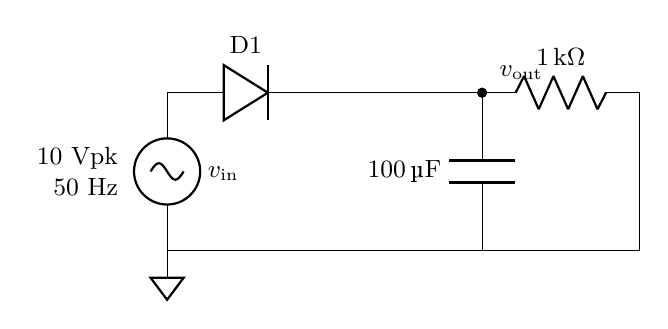
\begin{tikzpicture}[american, font=\small]
  \draw (0,0) node[sground]{};
  \draw (0,0) to[sV, l_=$v_{\mathrm{in}}$] (0,2)
        to[D, l=D1] (2,2) -- (4,2)
        to[C, l_={\qty{100}{\micro\farad}}, *-] (4,0) -- (0,0);
  \node[font=\small, left, align=right] at (-0.5,1.0) {10 Vpk\\50 Hz};
  \draw (4,2) to[R, l={\qty{1}{\kilo\ohm}}] (6,2) -- (6,0) -- (4,0);
  \node[circ] at (4,2) {}; \node[right, font=\small] at (4.1,2.25){$v_{\mathrm{out}}$};
\end{tikzpicture}\\[0.8em]
\begin{tikzpicture}
\begin{axis}[
  width=0.72\linewidth, height=4.6cm,
  xlabel={$t$ (ms)}, ylabel={V},
  xmin=40, xmax=100, ymin=-11, ymax=11,
  grid=both, tick label style={font=\small},
  legend style={font=\small, at={(0.03,0.30)}, anchor=west},
]
\addplot[gray] table[x index=0, y index=1] {figures/ch05/ch05_rectifier_ms.dat};
\addlegendentry{$v_{\mathrm{in}}$}
\addplot[blue, thick] table[x index=0, y index=2] {figures/ch05/ch05_rectifier_ms.dat};
\addlegendentry{$v_{\mathrm{out}}$ (C=\qty{100}{\micro\farad})}
\draw[dashed, red] (axis cs:40,9.19) -- (axis cs:100,9.19);
\draw[dashed, red] (axis cs:40,7.69) -- (axis cs:100,7.69);
\node[font=\small, anchor=west, text=red] at (axis cs:50,-4)
  {ripple $\approx$ \qty{1.5}{\volt} p-p};
\end{axis}
\end{tikzpicture}

\caption{Half-wave rectifier and its real \texttt{.tran} waveforms.
Notice the output is a decaying exponential between brief recharging
peaks, not a sine minus a piece. The diode only conducts for the short
window where $v_{\mathrm{in}}$ climbs above $v_{\mathrm{out}}+0.7$.}
\label{fig:rectifier}
\end{figure}

\begin{exercise}[medium]
Same rectifier, but the load is a \qty{10}{\milli\ampere} constant sink
and $C=\qty{220}{\micro\farad}$. Predict the p-p ripple.
\begin{solution}
$\Delta v\approx IT/C=10\text{m}\cdot20\text{m}/220\mu\approx\qty{0.9}{\volt}$.
(Constant current makes the linear estimate nearly exact --- no drooping
load to save you.)
\end{solution}
\end{exercise}

\section{The flyback diode: ch.~4's missing part}\label{sec:diode-flyback}

Chapter~4 opened a relay coil and watched the switch node jump to
\qty{1646}{\volt}. In a real circuit that spike lands on a transistor
rated for maybe \qty{40}{\volt} --- once. The fix is one diode across the
coil, \emph{freewheeling}: anode at the switched node, cathode at the
supply rail. While the coil is driven, the diode is reverse-biased and
invisible. The instant the switch opens, the coil's stored current keeps
flowing --- inductor current cannot jump --- and now it has somewhere to
go: through the diode, clamping the node at rail plus one drop.

\begin{lstlisting}[caption={\ttfamily code/ch05\_flyback\_diode.cir ---
identical to ch.~4's flyback netlist except one added line: \texttt{D1 3 1
DSI}. This diode is the difference between a circuit that works and a
dead transistor.},label=lst:flybackd]
* ch05_flyback_diode.cir -- ch4 relay coil with a freewheel diode
* WARNING: omitting this diode is what kills real transistors.
.model SW1 SW vt=0.5 vh=0.1 ron=1 roff=1e9
.model DSI D(is=1e-14 n=1.1 rs=0.5)
V1 1 0 dc 12
Rcoil 1 2 70
L1 2 3 10m IC=0
S1 3 0 10 0 SW1
Cpar 3 0 100p
D1 3 1 DSI
Vsw 10 0 pulse(1 0 1m 1n 1n 1 1)
.control
tran 500n 1.06m uic
wrdata ch05_flyback_diode.dat v(3) i(l1)
meas tran VPK MAX v(3)
.endc
.end
\end{lstlisting}

\begin{lstlisting}[caption={Output, verbatim. Same relay, same switch ---
the \qty{1646}{\volt} spike is gone.}]
vpk                 =  1.30279e+01 at=  1.00001e-03
\end{lstlisting}

\qty{13.0}{\volt}: rail plus one diode drop. The coil current decays
gently through the diode instead of detonating the voltage node.

\begin{figure}[htbp]
\centering
% fig_flybackdiode.tex -- freewheel diode placement + real clamped waveform
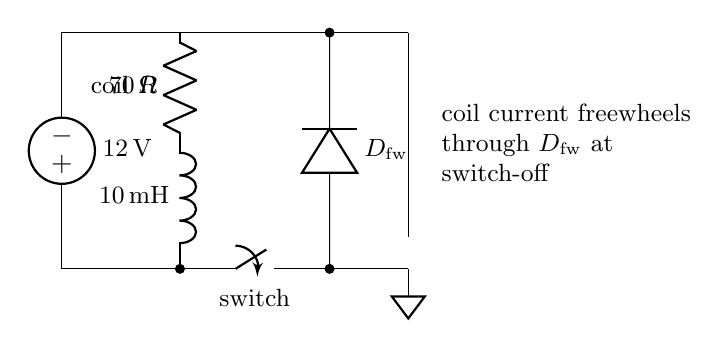
\begin{tikzpicture}[american, font=\small]
  \draw (0,0) to[V, l_={\qty{12}{\volt}}] (0,3) -- (1.5,3)
        to[R, l_={\qty{70}{\ohm}}, a={coil $R$}] (1.5,1.6);
  \draw (1.5,1.6) to[L, l_={\qty{10}{\milli\henry}}] (1.5,0.2) -- (1.5,0);
  \draw (1.5,0) to[cspst, l_={switch}] (3.4,0) -- (4.4,0) node[sground]{};
  \draw (0,0) -- (1.5,0);
  \draw (3.4,0) to[D, l_={$D_{\mathrm{fw}}$}] (3.4,3);
  \draw (1.5,3) -- (3.4,3) -- (4.4,3);
  \draw (4.4,3) -- (4.4,0.4);
  \node[circ] at (1.5,0){}; \node[circ] at (3.4,0){}; \node[circ] at (3.4,3){};
  \node[font=\small, align=left, anchor=west] at (4.7,1.6)
    {coil current freewheels\\through $D_{\mathrm{fw}}$ at\\switch-off};
\end{tikzpicture}\\[0.8em]
\begin{tikzpicture}
\begin{axis}[
  width=0.72\linewidth, height=4.6cm,
  xlabel={$t$ (ms)}, ylabel={$v_{\mathrm{sw}}$ (V)},
  xmin=0.95, xmax=1.06, ymin=0, ymax=15,
  grid=both, tick label style={font=\small},
  restrict y to domain=-1:20,
]
\addplot[blue, thick] table[x index=0, y index=1]
  {figures/ch05/ch05_flyback_diode_ms.dat};
\draw[dashed, red] (axis cs:0.95,13.03) -- (axis cs:1.06,13.03)
  node[pos=0.2, anchor=south, font=\small] {clamped at $\approx$\qty{13}{\volt}};
\node[font=\small, anchor=south west] at (axis cs:0.96,5.5)
  {without the diode: \qty{1646}{\volt} (ch.~4 sim)};
\end{axis}
\end{tikzpicture}

\caption{Freewheel diode placement and the real clamped waveform. Notice
the diode is \emph{backwards} --- it can never conduct while the switch
is on; it exists purely for the turn-off instant.}
\label{fig:flybackd}
\end{figure}

\begin{remark}
This is not a textbook scare story. Relay drivers, solenoid valves,
motor H-bridges and DC-DC converter switches all die this way in real
products --- the failure signature is a transistor that measures
shorted drain-to-source. Every bench engineer has a ``forgot the
flyback diode'' story; the part costs cents.
\end{remark}

\begin{exercise}[hard]
Pick a flyback diode rating for our relay: coil \qty{12}{\volt},
\qty{70}{\ohm} resistance, \qty{10}{\milli\henry}, switched by a
\qty{40}{\volt}-rated transistor.
\begin{solution}
Peak diode current = coil current at switch-off =
$12/70=\qty{171}{\milli\ampere}$. Peak reverse voltage = supply =
\qty{12}{\volt} (plus margin). Any diode rated $\ge$\qty{200}{\milli\ampere},
$\ge$\qty{25}{\volt} works --- a 1N4148 (200 mA, 75 V) is the classic
answer here; a 1N4007 if the coil were fat.
\end{solution}
\end{exercise}

\section{The zener and the shunt regulator}\label{sec:diode-zener}

A \emph{zener} is a diode manufactured to break down cleanly in
\emph{reverse}: above its rated $V_z$ it conducts hard, holding its
terminals near $V_z$. Use that flat spot as a voltage reference: feed it
through a series resistor, hang your load across the zener, and it
absorbs whatever current the load doesn't take. That is the \emph{shunt
regulator}.

\begin{definition}[Zener diode]\index{zener diode}\index{shunt regulator}
A diode run intentionally in reverse breakdown, where $v\approx V_z$
over a range of currents. The shunt regulator is a series resistor plus
a zener to ground: the resistor takes the rail-to-$V_z$ difference, the
zener takes the leftover current.
\end{definition}

\begin{example}[A \qty{3.3}{\volt} reference from \qty{9}{\volt}, sized and simulated]\label{ex:zener}
\textbf{Strategy.} Size $R_s$ so the zener still sees a few milliamps at
\emph{maximum} load (otherwise it drops out of breakdown), and so its
power is safe at \emph{zero} load (when it takes everything). Then
sweep the load current and look at what ``regulates'' really means.

\textbf{Solution.} Load: up to \qty{30}{\milli\ampere}. Give the zener
$\sim$\qty{2}{\milli\ampere} margin at full load:
$R_s=(9-3.3)/(30\text{m}+2\text{m})\approx\qty{180}{\ohm}$. Worst-case
resistor power at zero load: $(5.7)^2/180\approx\qty{0.18}{\watt}$ ---
a quarter-watt part is adequate, barely. Worst-case zener power:
$3.3\cdot30\text{m}\approx\qty{0.1}{\watt}$.

\begin{lstlisting}[caption={\ttfamily code/ch05\_zener.cir --- shunt
regulator; the \texttt{.dc} sweep drives a current source as the load
and records $v_{\mathrm{out}}$.},label=lst:zener]
* ch05_zener.cir -- 3.3 V zener shunt regulator from 9 V
.model DZ3V3 D(is=1e-14 n=1.0 rs=5 bv=3.3 ibv=0.02)
V1 1 0 dc 9
Rs 1 2 180
Dz 0 2 DZ3V3
IL 2 0 dc 0
.control
dc IL 0 0.03 0.0005
wrdata ch05_zener.dat -i(v1) v(2)
.endc
.end
\end{lstlisting}

\begin{lstlisting}[caption={Selected rows of the \texttt{.dc} sweep
(every 10th of 61): load current, total supply current, output voltage.
Notice $v_{\mathrm{out}}$ slides \qty{0.22}{\volt} end to end --- this is
regulation, not magic.}]
IL (mA)   supply I (mA)   vout (V)
0.0       30.75           3.465
10.0      31.07           3.407
20.0      31.43           3.343
30.0      31.95           3.250
\end{lstlisting}
\end{example}

\begin{figure}[htbp]
\centering
% fig_zener.tex -- zener shunt regulator schematic + real load regulation
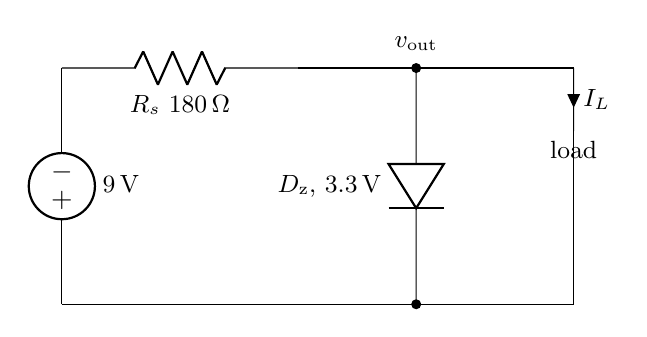
\begin{tikzpicture}[american, font=\small]
  \draw (0,0) to[V, l_={\qty{9}{\volt}}] (0,3);
  \draw (0,3) to[R, l_={$R_s$ \qty{180}{\ohm}}] (3,3);
  \draw (3,3) -- (4.5,3);
  \draw (4.5,3) to[D, a_={$D_{\mathrm{z}}$, \qty{3.3}{\volt}}] (4.5,0);
  \draw (0,0) -- (4.5,0);
  \draw (6.5,3) to[short, i=$I_L$] (6.5,2.2);
  \draw (4.5,3) -- (6.5,3);
  \draw (6.5,2.2) node[below, font=\small]{load} -- (6.5,1.4);
  \draw (6.5,1.4) -- (6.5,0) -- (4.5,0);
  \node[circ] at (4.5,3){}; \node[circ] at (4.5,0){};
  \node[above, font=\small] at (4.5,3.1){$v_{\mathrm{out}}$};
\end{tikzpicture}\\[0.8em]
\begin{tikzpicture}
\begin{axis}[
  width=0.72\linewidth, height=4.6cm,
  xlabel={load current $I_L$ (mA)}, ylabel={$v_{\mathrm{out}}$ (V)},
  xmin=0, xmax=30, ymin=3.0, ymax=3.6,
  grid=both, tick label style={font=\small},
]
\addplot[blue, thick] table[x index=0, y index=2] {figures/ch05/ch05_zener.dat};
\draw[dashed, gray] (axis cs:0,3.3) -- (axis cs:30,3.3)
  node[pos=0.65, anchor=south, font=\small] {nominal \qty{3.3}{\volt}};
\node[font=\small, anchor=west, align=left] at (axis cs:12,3.5)
  {\qty{3.47}{\volt}$\to$\qty{3.25}{\volt} over 30 mA:\\honest, not great};
\end{axis}
\end{tikzpicture}

\caption{Zener shunt regulator and its real load-regulation curve.
Notice the output sits \emph{above} \qty{3.3}{\volt} at light load and
sags below it at full load --- a low-voltage zener's knee is soft, so
``3.3 V'' is a neighborhood, not a number.}
\label{fig:zener}
\end{figure}

Honest verdict on the shunt regulator: it is simple, it is robust, it
wastes power continuously (the resistor burns $\sim$\qty{0.2}{\watt}
always), and it regulates loosely. Reach for it when you need a cheap
\emph{reference} for milliamps of bias or a comparator threshold ---
never for powering anything that cares.

\begin{exercise}[medium]
Your load can pull \qty{20}{\milli\ampere} and you want the zener to
keep $\ge$\qty{5}{\milli\ampere} at worst. What is the largest legal
$R_s$ from \qty{9}{\volt}, and what power must it survive at zero load?
\begin{solution}
$R_{s,\max}=(9-3.3)/(20\text{m}+5\text{m})=\qty{228}{\ohm}$ ---
pick \qty{220}{\ohm}. Zero-load power:
$(5.7)^2/220=\qty{0.15}{\watt}$, so a quarter-watt part survives with
40\% margin --- use a half-watt if the chassis gets hot.
\end{solution}
\end{exercise}

\section{The diode in the wild: ESD and reverse-polarity guards}\label{sec:diode-wild}

Two more jobs you will meet diodes doing on every board you open.
\emph{ESD protection}: tiny fast diodes from a signal line to each rail
clamp electrostatic hits (a finger is a few-kilovolt capacitor) before
they reach the chip. \emph{Reverse-polarity protection}: a diode in
series with the supply so a backwards plug or reversed battery does
nothing --- the diode blocks the negative rail outright.

The series guard costs you one forward drop, always. That is the whole
trade, quantified:

\begin{example}[Reverse-polarity protection: silicon vs Schottky vs no guard]\label{ex:revpol}
\textbf{Strategy.} Price the protection: what voltage does the load
lose forwards, what does it see backwards, and what power does the
diode burn. A Schottky diode trades a lower drop for looser blocking.

\textbf{Solution.} \qty{5}{\volt} supply, \qty{100}{\ohm} load
(\qty{50}{\milli\ampere} class), series diode:

\begin{lstlisting}[caption={\ttfamily code/ch05\_reverse\_pol.cir ---
\texttt{alter} re-runs the operating point with the supply flipped;
\texttt{ch05\_reverse\_pol\_sch.cir} swaps the silicon model for
Schottky.},label=lst:revpol]
* ch05_reverse_pol.cir -- series-diode reverse-polarity guard
.model DSI D(is=1e-14 n=1.1 rs=0.5)
V1 1 0 dc 5
D1 1 2 DSI
R1 2 0 100
.control
op
print v(1) v(2) i(v1)
alter v1 dc=-5
op
print v(1) v(2) i(v1)
.endc
.end
\end{lstlisting}

\begin{lstlisting}[caption={Outputs, verbatim: silicon forward,
reversed, then the Schottky run.}]
v(1) = 5.000000e+00   v(2) = 4.152554e+00   i = -4.15255e-02
v(1) = -5.00000e+00   v(2) = -5.01000e-10   i =  5.01110e-12
v(1) = 5.000000e+00   v(2) = 4.760269e+00   i = -4.76027e-02
\end{lstlisting}

Silicon: the load gets \qty{4.15}{\volt} and the diode burns
$0.85\cdot42\text{m}\approx\qty{36}{\milli\watt}$. Reversed: the load
sees $\sim$\qty{0}{\volt} and the circuit pulls picoamps. Schottky:
\qty{4.76}{\volt} delivered, only \qty{0.24}{\volt} sacrificed and
$\sim$\qty{11}{\milli\watt} burned. The trade: Schottkys leak more in
reverse and cost slightly more --- and ``just don't plug it in wrong''
remains the cheapest option on the table.
\end{example}

\section{Safety}\label{sec:diode-safety}

\begin{rulebox}
Rectifier circuits in this chapter are simulated at \qty{10}{\volt} and
lower. Real rectifiers live next to mains --- that is out of scope for
this book, full stop. The same diode that is a gentle one-way valve at
\qty{5}{\volt} is part of a lethal circuit at \qty{230}{\volt}.
\end{rulebox}

\begin{rulebox}
An inductor with no freewheel path does not negotiate --- it makes the
voltage it needs. Never switch a relay, solenoid, or motor coil without
the diode fitted first, and never trust a ``it worked on the bench''
argument: the transistor fails on the Nth switch, not the first.
\end{rulebox}

\section{Common mistakes}\label{sec:diode-mistakes}

\begin{tripwire}[Treating the diode as a zero-volt drop]
The ideal model is for direction questions only. The \qty{0.7}{\volt}
the load never sees is also power the diode has to dissipate ---
\qty{1}{\ampere} through a series guard is \qty{0.7}{\watt} to heat.
\end{tripwire}

\begin{tripwire}[Forgetting the reverse-voltage limit]
Every diode has a peak inverse voltage rating (1N4007: \qty{1000}{\volt};
a small-signal diode may only manage \qty{75}{\volt}). Exceed it and the
diode breaks down --- sometimes usefully (a zener), usually not (it
fails shorted).
\end{tripwire}

\begin{tripwire}[Sizing LED current off the ideal model]
``The diode drops zero, so $R=V/I$'' leaves nothing for the LED's real
\qty{1.8}{\volt}--\qty{3.4}{\volt} $V_f$. Always subtract $V_f$ first ---
and get it from the datasheet, because colour sets the voltage.
\end{tripwire}

\begin{tripwire}[Believing a zener holds its rated voltage]
Low-voltage zeners have soft knees: our ``3.3 V'' part delivered
\qty{3.25}{\volt} to \qty{3.47}{\volt} across the load range. If your
circuit cares about 6\%, you need a real reference IC, not a shunt
regulator.
\end{tripwire}

\section{Summary}\label{sec:diode-summary}

\begin{center}
\begin{tabularx}{\textwidth}{l>{\raggedright\arraybackslash}X}
\toprule
\textbf{Object} & \textbf{What you need to know}\\
\midrule
Diode models & ideal (0 V) for direction; \qty{0.7}{\volt} for hand
math; Shockley exponential in the simulator \\
LED & a diode that emits; $V_f$ is colour-set,
\qty{1.8}{\volt}--\qty{3.4}{\volt} --- read the datasheet \\
Rectifier & half-wave: one diode; cap filters gaps;
$\Delta v\lesssim IT/C$ p-p ripple; more $C$, less ripple \\
Flyback diode & across the coil, backwards; clamps switch-off spike at
rail+drop --- never optional \\
Zener & reverse breakdown held at $V_z$; shunt regulator = $R_s$ +
zener; loose ($\pm$5--10\%), always dissipating \\
Guards & series diode blocks reversed supply at one drop; Schottky
halves the toll; ESD diodes clamp signal pins to the rails \\
\bottomrule
\end{tabularx}
\end{center}

\section*{Exercises}
\addcontentsline{toc}{section}{Exercises}

\begin{exercise}[easy]
An ideal-model analysis says a diode drops nothing. Your circuit feeds
\qty{9}{\volt} through one diode to a \qty{3}{\volt} zener clamp. What
does the \qty{0.7}{\volt} model say the clamp sees? When does the 0.7 V
matter?
\end{exercise}

\begin{exercise}[easy]
Green LED, $V_f=\qty{2.1}{\volt}$, from \qty{3.3}{\volt} at
\qty{8}{\milli\ampere}: size the resistor.
\end{exercise}

\begin{exercise}[easy]
Which model do you use to (a) decide whether a diode conducts at all,
(b) size a series resistor by hand, (c) check a circuit in ngspice?
\end{exercise}

\begin{exercise}[easy]
In a half-wave rectifier, which half of the AC cycle appears at the
output --- and what decides which half? Trace the current path for the
conducting half.
\end{exercise}

\begin{exercise}[medium]
A rectifier must hold ripple under \qty{0.5}{\volt} p-p at
\qty{20}{\milli\ampere}, \qty{50}{\hertz}. What is the smallest
capacitor the linear estimate allows?
\end{exercise}

\begin{exercise}[medium]
Why is $\Delta v\approx IT/C$ an \emph{overestimate} of the ripple for
a resistive load but nearly exact for a constant-current load?
\end{exercise}

\begin{exercise}[medium]
A relay coil: \qty{24}{\volt}, \qty{15}{\milli\henry}, \qty{120}{\ohm},
switched at \qty{10}{\hertz}. Specify a flyback diode (current and
reverse-voltage rating with margin) and estimate the energy dissipated
per switch-off.
\end{exercise}

\begin{exercise}[medium]
A \qty{4.3}{\volt}-logic board must survive reversed \qty{5}{\volt}
input. Compare series silicon diode, series Schottky, and ``no guard''
on delivered voltage and dissipation at \qty{100}{\milli\ampere}.
\end{exercise}

\begin{exercise}[hard]
An LED matrix row drives 8 parallel LEDs ($V_f=\qty{2.0}{\volt}$ each)
from \qty{5}{\volt} through one shared resistor. Why is one resistor
per LED the correct design instead? (Hint: what happens to current
sharing when one LED's $V_f$ is \qty{0.1}{\volt} low?)
\end{exercise}

\begin{exercise}[hard]
Design a zener reference for \qty{5.1}{\volt} $\pm$\qty{0.2}{\volt}
into a load of \qty{0}{\milli\ampere}--\qty{10}{\milli\ampere} from a
\qty{12}{\volt} rail: choose $R_s$, bound the zener and resistor power,
and estimate the real output range given our measured low-$V_z$ slope
($\sim$\qty{7}{\milli\volt}/mA).
\end{exercise}

\section*{Hints and answers}
\addcontentsline{toc}{section}{Hints and answers}

\begin{description}
\item[Clamp after diode.] $9-0.7=\qty{8.3}{\volt}$ across $R_s$, so the
zener sees slightly less drive current --- the drop matters when $R_s$
is tight or the rail is low; it's why low-voltage designs use Schottky.
\item[Green LED.] $R=(3.3-2.1)/0.008=\qty{150}{\ohm}$.
\item[Model picking.] (a) ideal, (b) \qty{0.7}{\volt} (or LED $V_f$),
(c) Shockley --- the simulator never uses your shortcuts.
\item[Rectifier half.] Whichever half forward-biases the diode ---
anode side positive. Flip the diode to pick the other half.
\item[Ripple cap.] $C\ge IT/\Delta v=20\text{m}\cdot20\text{m}/0.5
=\qty{800}{\micro\farad}$ --- the estimate is an upper bound on ripple,
so this is conservative; buy \qty{1000}{\micro\farad}.
\item[Overestimate.] Resistive load current sags with the voltage, so
the bucket empties slower than $I\cdot t$ assumes; a constant-current
load never sags, so the linear discharge is real.
\item[24 V relay.] $I_{\mathrm{pk}}=24/120=\qty{200}{\milli\ampere}$;
diode $\ge$\qty{250}{\milli\ampere}, $\ge$\qty{50}{\volt} (e.g.
1N4001). Energy per switch-off:
$\frac12 LI^2=\frac12\cdot0.015\cdot0.2^2=\qty{0.3}{\milli\joule}$ ---
at \qty{10}{\hertz}, \qty{3}{\milli\watt} in the diode loop.
\item[Reversed guard.] At \qty{100}{\milli\ampere}: silicon delivers
$\approx$\qty{4.15}{\volt} and burns $\approx$\qty{85}{\milli\watt};
Schottky $\approx$\qty{4.76}{\volt}, $\approx$\qty{24}{\milli\watt};
no guard delivers \qty{5}{\volt} and dies if someone plugs it in wrong.
\item[LED matrix.] A shared resistor sets total current but the LED
with the lowest $V_f$ hogs it --- exponential $I$--$V$ means
\qty{0.1}{\volt} low doubles its share. One resistor per LED fixes
each branch's own current.
\item[5.1 V reference.] $R_s\le(12-5.1)/15\text{m}=\qty{460}{\ohm}$;
pick \qty{430}{\ohm}. Resistor power $(6.9)^2/430\approx\qty{0.11}{\watt}$;
zener worst case $5.1\cdot16\text{m}\approx\qty{0.08}{\watt}$.
At $\sim$\qty{7}{\milli\volt}/mA the output stays inside
$\pm$\qty{0.2}{\volt} up to $\sim$28 mA of load swing --- yours has 10.
Feasible.
\end{description}

\section*{Notes}
\addcontentsline{toc}{section}{Notes}

\chapternotes{%
The three-models presentation and the Shockley-stated-not-derived choice
follow the layered-model approach of the 6.002 nonlinear lectures
\cite{ocw6002} and All About Circuits vol.~III's diode chapter
\cite{aacvol3}. The flyback-diode-as-required-instrument framing is
standard bench practice; the simulated spike and clamp are real ngspice
runs of the relay from ch.~4. Zener knee softness at low $V_z$ is a
documented device property, which is why the chapter's regulator verdict
is honest rather than enthusiastic \cite{aacvol3}.}

\begin{wins}
\begin{itemize}
\item Read a diode $I$--$V$ curve and pick the right model for the job.
\item Predict and verify rectifier ripple; know why $IT/C$ overestimates.
\item Add the flyback diode to any inductive switch --- and justify its rating.
\item Build and honestly evaluate a zener shunt reference.
\item Price reverse-polarity protection in volts and milliwatts.
\end{itemize}
\end{wins}

\chapter{Transistors: the switch and the amplifier}
\label{ch:transistors}

Everything digital in this book — logic gates, the FPGA fabric you will
program later — is built from one trick, repeated a billion times: a voltage
that controls another current. This chapter introduces the transistor as a
\emph{switch} first (the model you will actually use), then as an
\emph{amplifier} in one honestly-flagged example. When you finish, you will
be able to read a voltage-transfer curve for noise margins, explain why CMOS
logic draws almost no power at rest, and decide whether a given MOSFET can
really drive a given load from a \qty{3.3}{\volt} pin.

% from-zero:begin
\begin{rulebox}[Before you start]
Chapters~2 and~5. \emph{Recap:} a transistor is a switch that another voltage or current controls. Everything digital in this book is made of them.
\end{rulebox}
\begin{wins}[After this chapter you can]
\begin{itemize}
\item explain how a MOSFET works as a voltage-controlled switch;
\item build an inverter and explain why CMOS draws almost no power at rest;
\item read a logic level as ``1'' or ``0'' with noise margins;
\item drive a real load such as a motor or LED with a transistor.
\end{itemize}
\end{wins}
\begin{principle}[How to think about this]
A transistor is a valve: a small signal at the control terminal opens or closes a large path. Use it as a switch and you get digital logic; use it in between and you get amplification. CMOS pairs two complementary valves so that one is always closed, which is why idle chips use almost no power.
\end{principle}
% from-zero:end

\section{The MOSFET: a voltage-controlled switch}
\label{sec:mosfet}

The \emph{MOSFET}\index{MOSFET} (metal-oxide-semiconductor field-effect
transistor) has three terminals we care about — \emph{gate} ($G$),
\emph{drain} ($D$), \emph{source} ($S$) — drawn in
Figure~\ref{fig:mosfet}. The gate sits on an insulating oxide layer: it
controls the device by \emph{electric field}, not by current, so an ideal
gate draws no DC current at all.

\begin{figure}[htbp]
\centering
\begin{tikzpicture}
  % NMOS symbol with terminals labelled and body diode noted
  \node[nmos, scale=1.4](Q) at (2,1.5) {};
  \node[left] at (Q.G) {gate $G$};
  \node[above right] at (Q.D) {drain $D$};
  \node[below right] at (Q.S) {source $S$};
  \draw[->, accent, thick] ($(Q.G)+(-0.6,0)$) -- ($(Q.G)+(-0.1,0)$);
  \node[anchor=west, align=left, font=\small] at (3.6,1.5)
    {$v_{GS} > V_{th}$: channel conducts $D \leftrightarrow S$\\
     gate draws (almost) no DC current};
\end{tikzpicture}

\caption{An NMOS transistor and its three terminals. Notice what the gate
does \emph{not} do: it draws essentially no DC current — it works by field,
not by flow.}
\label{fig:mosfet}
\end{figure}

\begin{definition}[NMOS threshold]
\index{threshold voltage}
An NMOS\index{NMOS} device conducts between drain and source when the
\emph{gate-source voltage} exceeds a device constant $V_{th}$, the
\emph{threshold voltage} (a volt or two for small-signal parts). Below
$V_{th}$ the channel is essentially open.
\end{definition}

The 6.002 pedagogy layers two models on this~\cite{ocw6002}:

\begin{definition}[S and SR models]
\index{MOSFET!S model}\index{MOSFET!SR model}
The \emph{S (switch) model}: $v_{GS} > V_{th}$ $\Rightarrow$ drain and
source are a wire; otherwise an open circuit. The \emph{SR (switch-resistor)
model}: on, the channel behaves as a small resistance $R_{on}$ instead of an
ideal wire — the model you reach for once a load current flows.
\end{definition}

\begin{figure}[htbp]
\centering
\begin{circuitikz}[american]
  % S model: ideal switch
  \node[above] at (1,3.2) {\small\textbf{S model}};
  \draw (1,3) node[circ]{} node[left]{$D$} to[cspst, l_={\scriptsize$v_{GS}>V_{th}$}] (1,1);
  \draw (1,1) node[left]{$S$} node[circ]{};
  \node[align=left, font=\small] at (1,-0.4) {on: wire\\ off: open};
  % SR model: switch + R_on
  \node[above] at (5,3.2) {\small\textbf{SR model}};
  \draw (5,3) node[circ]{} node[left]{$D$} to[cspst, l_={\scriptsize$v_{GS}>V_{th}$}] (5,2)
        to[R, l_=$R_{on}$, -*] (5,0.6) node[left]{$S$} node[circ]{};
  \node[align=left, font=\small] at (5,-0.4) {on: $R_{on}$ (ohms, not zero)\\ off: open};
\end{circuitikz}

\caption{The two switch models. Use S to reason about logic levels; use SR
the moment real current must flow, because $R_{on}$ drops real volts.}
\label{fig:ssr}
\end{figure}

\begin{remark}
Gate current is not literally zero — charging the gate capacitance takes
charge, which is why fast switching burns power (Section~\ref{sec:cmos})
and why FPGAs get warm. "No DC gate current" is a DC statement.
\end{remark}

\section{The NMOS inverter, built by hand}
\label{sec:nmosinv}

Pull the drain up to $V_{DD}$ through a resistor and drive the gate with the
input: when $v_{in} > V_{th}$ the channel conducts and drags the output
down; below threshold the resistor pulls the output up. That is an
\emph{inverter}\index{inverter (logic)} — input 1 gives output 0 and vice
versa. Figure~\ref{fig:vtc} plots its \emph{voltage-transfer
characteristic}\index{voltage-transfer characteristic} (VTC).

\begin{example}[Reading noise margins off a real VTC]\label{ex:vtc}
\textbf{Strategy.} Simulate the NMOS + \qty{10}{\kilo\ohm} pull-up inverter,
then read the four landmarks: the flat output levels $V_{OH}$/$V_{OL}$ and
the input voltages $V_{IL}$/$V_{IH}$ where the curve leaves those flats
(the unit-slope points, read approximately).

\textbf{Solution.} The netlist and the transfer data:
\end{example}

\begin{lstlisting}[caption={\ttfamily code/ch06\_nmos\_inv.cir --- NMOS inverter with a resistive pull-up.},label=lst:nmosinv]
* ch06_nmos_inv.cir -- NMOS + pull-up resistor inverter, .dc transfer
VDD 3 0 dc 3.3
Vin 1 0 dc 0
M1 2 1 0 0 NMOS1 W=10u L=1u
RD 3 2 10k
.model NMOS1 NMOS(vto=1.0 kp=200u lambda=0.02)
.control
dc Vin 0 3.3 0.025
set filetype=ascii
wrdata ch06_nmos_inv.dat v(2)
* static supply current at vin = 3.3 V (inverter holding "low")
dc Vin 3.3 3.3 0.01
print i(VDD)
.endc
.end
\end{lstlisting}

\begin{lstlisting}[language={},caption={Rows of \texttt{ch06\_nmos\_inv.dat}, verbatim --- read $V_{OH}$, $V_{OL}$, and where the knee sits.},label=lst:nmosdata]
vin        vout
0.500      3.3000
1.000      3.3000
1.250      2.6420
1.500      0.7619
1.750      0.2419
2.000      0.1705
3.000      0.0820
3.300      0.0712
\end{lstlisting}

Reading Figure~\ref{fig:vtc}: $V_{OH}=\qty{3.30}{\volt}$,
$V_{OL}\approx\qty{0.07}{\volt}$, $V_{IL}\approx\qty{1.2}{\volt}$ (output
just starting to fall), $V_{IH}\approx\qty{1.7}{\volt}$ (output nearly
bottomed). The margins of Definition~\ref{def:noisemargin} are then
$N M_L \approx 1.2-0.07 \approx \qty{1.1}{\volt}$ and
$N M_H \approx 3.3-1.7 \approx \qty{1.6}{\volt}$.

\begin{figure}[htbp]
\centering
\begin{tikzpicture}
\begin{axis}[width=11cm,height=6.5cm, xlabel={$v_{in}$ (V)}, ylabel={$v_{out}$ (V)},
  xmin=0,xmax=3.3, ymin=0,ymax=3.4, grid=both, legend pos=north east,
  every axis plot/.append style={thick}]
  \addplot[blue] table {figures/ch06/ch06_nmos_inv.dat};
  \addlegendentry{NMOS + $10\,\mathrm{k}\Omega$ pull-up}
  \addplot[red] table {figures/ch06/ch06_cmos_inv.dat};
  \addlegendentry{CMOS}
  % noise-margin landmarks on the NMOS curve
  \draw[dashed, slate] (axis cs:1.2,0) -- (axis cs:1.2,3.3);
  \draw[dashed, slate] (axis cs:1.7,0) -- (axis cs:1.7,3.3);
  \draw[dashed, slate] (axis cs:0,0.071) -- (axis cs:3.3,0.071);
  \node[font=\scriptsize, anchor=west] at (axis cs:0.05,0.45) {$V_{OL}\approx0.07$};
  \node[font=\scriptsize, rotate=90, anchor=south] at (axis cs:1.2,1.0) {$V_{IL}\approx1.2$};
  \node[font=\scriptsize, rotate=90, anchor=south] at (axis cs:1.7,1.0) {$V_{IH}\approx1.7$};
  \node[font=\scriptsize, anchor=west] at (axis cs:0.05,3.15) {$V_{OH}=3.30$};
\end{axis}
\end{tikzpicture}

\caption{Measured inverter transfer curves (both real \texttt{.dc} sweeps).
Notice how much cleaner the CMOS knee is: it snaps over near $V_{DD}/2$ and
actually reaches the rails.}
\label{fig:vtc}
\end{figure}

\section{The static discipline: what makes a level a ``1''}
\label{sec:staticdisc}

Digital only works if stages can be chained: the output of one inverter must
be read correctly by the input of the next, with slack for real-world noise.

\begin{definition}[Static discipline and noise margins]
\label{def:noisemargin}
\index{static discipline}\index{noise margin}
A logic family fixes four voltages: a sender guarantees $v \le V_{OL}$
(``0'') or $v \ge V_{OH}$ (``1''); a receiver accepts $v \le V_{IL}$ as 0
and $v \ge V_{IH}$ as 1, with $V_{OL} < V_{IL} < V_{IH} < V_{OH}$. The gaps
are the \emph{noise margins} $NM_L = V_{IL}-V_{OL}$ and
$NM_H = V_{OH}-V_{IH}$ — how much corruption a wire can absorb before a bit
flips.
\end{definition}

\begin{exercise}[easy]
On Figure~\ref{fig:vtc}'s NMOS curve, is \qty{0.8}{\volt} a safe ``0''
input? Is \qty{1.4}{\volt} a safe ``1'' input? (Use the landmarks just
computed.)
\end{exercise}

\section{CMOS: the pair that draws no power at rest}
\label{sec:cmos}

The resistor pull-up has a defect you can see in the netlist's own printout:
holding the output low means burning $V_{DD}/R$ forever.

\begin{lstlisting}[language={},caption={Last lines of \texttt{ngspice -b ch06\_nmos\_inv.cir} --- the static current while holding output low.}]
i(vdd) = -3.22881e-04
\end{lstlisting}

\qty{0.32}{\milli\ampere} continuously, \emph{per inverter}, for doing
nothing. \emph{CMOS}\index{CMOS} (complementary MOS) replaces the resistor
with a \emph{PMOS}\index{PMOS} transistor — same device, but conducting when
$v_{GS} < V_{th} < 0$, i.e. when the gate is \emph{low}. Now the pull-up is
on exactly when the pull-down is off (Figure~\ref{fig:cmos}): one transistor
of the pair always blocks the rail-to-ground path.

\begin{figure}[htbp]
\centering
\begin{circuitikz}[american, scale=0.9, transform shape]
  % CMOS inverter: PMOS pull-up + NMOS pull-down
  \node[above] at (1.2,4.9) {\small\textbf{inverter}};
  \draw (1.2,4.4) node[pmos, anchor=D](P){};
  \draw (1.2,1.2) node[nmos, anchor=D](N){};
  \draw (P.S) -- (N.D);
  \draw ($(P.S)!.5!(N.D)$) node[circ]{} to[short,-o] ++(1.4,0) node[right]{$Y=\overline{A}$};
  \draw (P.G) -- ++(-0.6,0) |- ($(P.G)!.5!(N.G)+(-0.6,0)$) -- (N.G) ++(-0.6,0);
  \draw ($(P.G)!.5!(N.G)+(-0.6,0)$) node[circ]{} to[short,-o] ++(-0.8,0) node[left]{$A$};
  \draw (N.S) node[ground]{};
  \draw (P.D) ++(0,0.4) node[vdd]{$V_{DD}$} -- (P.D);
  % CMOS NAND: PMOS pair in parallel on top, NMOS pair in series below
  \node[above] at (7.6,4.9) {\small\textbf{NAND}};
  \draw (6.4,4.0) node[pmos, anchor=D](P1){};
  \draw (8.6,4.0) node[pmos, anchor=D](P2){};
  \draw (P1.D) -- ++(0,0.5) -| (P2.D);
  \draw (P1.S) -- (P2.S);
  \draw (7.4,3.6) node[nmos, anchor=D](N1){};
  \draw (7.4,1.6) node[nmos, anchor=D](N2){};
  \draw (N1.S) -- (N2.D);
  \draw (P1.S) -- (N1.D);
  \draw ($(P1.S)!.5!(P2.S)$) node[circ]{} to[short,-o] ++(0.8,0) node[right]{$Y=\overline{A\cdot B}$};
  \draw (N2.S) node[ground]{};
  \draw ($(P1.D)+(0,0.5)$) to[short,-*] ++(0,0.2) node[vdd]{$V_{DD}$};
  \draw (P1.G) to[short,-o] ++(-0.9,0) node[left]{$A$};
  \draw (P2.G) to[short,-o] ++(0.9,0) node[right]{$B$};
  \draw (N1.G) to[short,-o] ++(-0.9,0) node[left]{$A$};
  \draw (N2.G) to[short,-o] ++(-0.9,0) node[left]{$B$};
\end{circuitikz}

\caption{The CMOS inverter (left) and a 2-input CMOS NAND (right): NMOS
network pulls down, PMOS network pulls up, and exactly one network conducts
for any input. Notice the NAND structure — series NMOS (both inputs needed
to pull down), parallel PMOS (either input high pulls up).}
\label{fig:cmos}
\end{figure}

\begin{example}[CMOS static power, measured]\label{ex:cmospower}
\textbf{Strategy.} Sweep the CMOS inverter and read the supply current at
the two resting points — the claim is that both are ~zero, with current only
\emph{during} transitions.

\textbf{Solution.} \texttt{code/ch06\_cmos\_inv.cir} prints
\texttt{i(VDD)} at $v_{in}=0$ and $v_{in}=\qty{3.3}{\volt}$:
\end{example}

\begin{lstlisting}[language={},caption={Static points of the CMOS sweep --- compare with the NMOS inverter's \qty{0.32}{\milli\ampere}.}]
i(vdd) = -3.31000e-12      (vin = 0)
i(vdd) = -3.31000e-12      (vin = 3.3)
\end{lstlisting}

Three picoamps — numerical noise, not real current. Meanwhile the mid-sweep
peak is $\qty{0.33}{\milli\ampere}$ at $v_{in}\approx\qty{1.6}{\volt}$: the
brief window where \emph{both} devices are part-on. That is the whole power
story of modern silicon: \textbf{CMOS burns energy only while
switching}\index{CMOS!power}, which is why processor power scales with
clock frequency.

\begin{principle}[Why CMOS won]
The complementary pair gets rail-to-rail outputs (0 and $V_{DD}$ exactly,
see Figure~\ref{fig:vtc}), a steep transition centred near $V_{DD}/2$, and
zero static current. Resistive pull-ups lose on all three.
\end{principle}

NOR gates swap the networks (parallel NMOS below, series PMOS above).
Every logic function you will meet is these two dual networks — a fact the
FPGA chapters lean on hard.

\begin{exercise}[medium]
Sketch the transistor-level structure of a 2-input CMOS NOR: which devices
are in series and which in parallel, and why must it be the dual of NAND?
\end{exercise}

\section{The BJT: the current-controlled cousin}
\label{sec:bjt}

The \emph{bipolar junction transistor}\index{BJT} (NPN/PNP) controls
collector current with a \emph{base current}: $i_C = \beta\, i_B$, with
$\beta$ of order 100. The mental model shift matters: a MOSFET answers
voltage, a BJT answers \emph{current} — you must supply base current
continuously, which is why discrete switch circuits prefer MOSFETs. BJTs
remain excellent small-signal amplifiers and live inside every op-amp; this
book treats them conceptually only (full biasing design is AoE territory,
flagged honestly).

\section{The transistor as amplifier}
\label{sec:amplifier}

Between "fully on" and "fully off" lies the region the VTC shows as a steep
slope: small changes in $v_{GS}$ produce large changes in $v_{DS}$ — gain.
Bias a single transistor mid-slope, feed it a small signal, and the same
device amplifies. We do exactly one example and then point onward.

\begin{example}[The inverter is also a (bad) amplifier]\label{ex:amp}
\textbf{Strategy.} The VTC slope $-dv_{out}/dv_{in}$ \emph{is} the small-signal
voltage gain. Estimate it from Figure~\ref{fig:vtc}'s steepest point.

\textbf{Solution.} The NMOS curve falls from $\approx\qty{2.6}{\volt}$ to
$\approx\qty{0.76}{\volt}$ between $v_{in}=\qty{1.25}{\volt}$ and
\qty{1.5}{\volt}: a local gain of about $-7$. Biased at
$v_{in}=\qty{1.4}{\volt}$, this inverter is a genuine inverting amplifier —
a terrible one (the bias point wanders with temperature and the pull-up
wastes power), but the same small-signal idea underlies every real
amplifier stage. The art of making this robust — feedback, biasing
networks, differential pairs — is where this book hands you to
AoE~\cite{aacvol3}.
\end{example}

\begin{exercise}[easy]
From the CMOS curve in Figure~\ref{fig:vtc}, estimate its maximum slope in
V/V. Why does a steeper transition make a better gate \emph{and} a better
(though twitchier) amplifier?
\end{exercise}

\section{Driving a load: the switch, for real}
\label{sec:switchload}

\begin{example}[A 2N7000-class MOSFET switching a \qty{12}{\volt} LED strip from \qty{3.3}{\volt} logic]\label{ex:gate}
\textbf{Strategy.} Low-side switch (Figure~\ref{fig:lowhigh}): load between
+\qty{12}{\volt} and drain, source grounded, gate to the logic pin. The
question is never "does it conduct" — it is "does it conduct
\emph{enough}" at the $v_{GS}$ you can actually supply. Check $V_{th}$
against your rail, then simulate the gate-drive sweep.

\textbf{Solution.} \texttt{code/ch06\_switch\_load.cir} sweeps the gate of a
$V_{th}=\qty{2.1}{\volt}$ device driving a \qty{600}{\ohm} strip
($\approx\qty{20}{\milli\ampere}$):
\end{example}

\begin{lstlisting}[language={},caption={Gate-drive sweep, verbatim rows --- the transistor turns on only gradually, and \qty{3.3}{\volt} drive leaves it half-on.},label=lst:switchload]
gate        drain
0.500       12.000
2.000       12.000
3.000        8.061
3.300        5.184
5.000        0.479
\end{lstlisting}

At $v_{GS}=\qty{3.3}{\volt}$ the overdrive is only
$3.3-2.1=\qty{1.2}{\volt}$: the channel passes \qty{11.4}{\milli\ampere}
while the load wants 20 — the strip glows at half brightness and the
transistor eats \qty{5.2}{\volt} of drop. At \qty{5}{\volt} drive the drain
sits at \qty{0.48}{\volt}: solidly on. \textbf{The lesson: match the FET's
specified $R_{on}$ to the gate voltage you actually have} — logic-level
parts specify $R_{on}$ at $v_{GS}=\qty{2.5}{\volt}$ or
\qty{1.8}{\volt} for exactly this reason.

\begin{figure}[htbp]
\centering
\begin{circuitikz}[american, scale=0.9, transform shape]
  % low-side: NMOS between load and ground
  \node[above, align=center] at (1.5,3.6) {\small\textbf{low-side} (ours)};
  \draw (0,3.2) node[vcc]{12 V} to[R, l_={load}] (0,1.8) -- (1.5,1.8);
  \draw (1.5,0.6) node[nmos, anchor=S](M){};
  \draw (M.D) -- (1.5,1.8);
  \draw (M.S) node[ground]{};
  \draw (M.G) to[short,-o] ++(-1.2,0) node[left]{3.3 V logic};
  \node[align=left, font=\small, anchor=west] at (3.0,1.2) {load keeps 12 V on top;\\source on ground --- easy gate drive};
  % high-side: switch above the load
  \node[above, align=center] at (8.5,3.6) {\small\textbf{high-side}};
  \draw (7,3.2) node[vcc]{12 V} -- (8.5,3.2);
  \draw (8.5,2.4) node[nmos, anchor=D](H){};
  \draw (8.5,3.2) -- (H.D);
  \draw (H.S) to[R, l_={load}] (8.5,0) node[ground]{};
  \draw (H.G) to[short,-o] ++(-1.2,0) node[left]{drive};
  \node[align=left, font=\small, anchor=west] at (10.0,1.2) {source rides the load ---\\gate must go \emph{above} the rail};
\end{circuitikz}

\caption{Low-side versus high-side switching. Notice why we always reach
for low-side first: with the source on ground, a \qty{3.3}{\volt} pin is a
known $v_{GS}$; high-side, the source rides the load and the gate needs a
voltage \emph{above the rail} (a bootstrap or charge pump — later study).}
\label{fig:lowhigh}
\end{figure}

\begin{checkpoint}
\textbf{Gate ESD.}\index{ESD!gate} The gate is a few nanometres of oxide; a
charged finger punctures it. Handle MOSFETs and CMOS ICs with static care,
and never leave a gate floating — tie it with a pull-down resistor so the
switch cannot turn on from noise. And this is why Chapter~\ref{ch:transients}'s
flyback diode matters here: the transistor switching a relay coil is
exactly the device the spike kills.
\end{checkpoint}

\begin{rulebox}[High-current switching]
Breadboards and jumper wires are rated for $\sim$\qty{1}{\ampere}. We
simulate anything beyond that — the physics of a \qty{20}{\ampere} switch is
identical, the burns are not.
\end{rulebox}

\section{Logic families and voltage levels}
\label{sec:levels}

Legacy TTL and \qty{5}{\volt} CMOS still exist, but this book lives at
\qty{3.3}{\volt}: modern FPGAs, microcontrollers and the Tang Nano all run
it, and mixing families costs you level shifters\index{level shifter} and
noise-margin headaches. The VTC numbers of Figure~\ref{fig:vtc} are why a
\qty{3.3}{\volt} input is \emph{not} automatically a valid 1 at a
\qty{5}{\volt} input — read the destination's $V_{IH}$ before connecting.

\begin{figure}[htbp]
\centering
\begin{tikzpicture}[font=\small]
  \draw[rounded corners, fill=slate!10] (0,0) rectangle (3,2.4);
  \node[align=center] at (1.5,1.2) {\textbf{analog world}\\ $v(t)$ continuous\\ noise accumulates};
  \draw[rounded corners, fill=accent!12] (5.5,0) rectangle (8.5,2.4);
  \node[align=center] at (7,1.2) {\textbf{digital world}\\ only two levels\\ \texttt{0} / \texttt{1}};
  \draw[->, very thick] (3.2,1.2) -- (5.3,1.2)
    node[midway, above, align=center, font=\small]{static discipline\\ $V_{IL},V_{IH},V_{OL},V_{OH}$\\ + noise margins};
\end{tikzpicture}

\caption{The bridge this chapter builds: analog voltage in, two clean
levels out — guaranteed by the static discipline, not by hope.}
\label{fig:bridge}
\end{figure}

\section{Common mistakes}
\label{sec:transistor-mistakes}

\begin{tripwire}[{Treating $V_{th}$ as a sharp on/off}]
Conduction is gradual (the switch-load sweep rises through 8 V, 5 V on its
way down). "Above threshold" means \emph{starting} to conduct; enough
current for your load is a separate question.
\end{tripwire}

\begin{tripwire}[{Swapping source and drain}]
A discrete NMOS's body diode\index{body diode} points source$\to$drain:
wired backwards, it conducts through the diode no matter what the gate
says. Power packages put a visible diode in the datasheet drawing — look
for it.
\end{tripwire}

\begin{tripwire}[{Leaving the gate floating}]
An un-driven gate drifts on leakage and switches at random — the ESD/gate
checkpoint's pull-down resistor is not decoration.
\end{tripwire}

\begin{tripwire}[{Assuming zero resistance when "on"}]
$R_{on}$ is real: Example~\ref{ex:gate}'s \qty{0.48}{\volt} drain drop at
full drive is \qty{9.6}{\milli\watt} of heat on a small part — check it
before claiming "switch closed".
\end{tripwire}

\section{Summary}
\label{sec:transistor-summary}

\begin{tabularx}{\linewidth}{l X}
\toprule
Concept & Takeaway \\
\midrule
S / SR models & on = wire, or wire + $R_{on}$; off = open \\
VTC & the curve that decides every digital level \\
Noise margins & $NM_L = V_{IL}-V_{OL}$, $NM_H = V_{OH}-V_{IH}$ \\
CMOS & complementary pair, ~0 static power, rail-to-rail \\
Gate drive & $v_{GS}-V_{th}$ sets how \emph{hard} the switch is on \\
Low-side first & source grounded $\Rightarrow$ easy drive \\
Amplifier & same device, biased mid-slope; details live in AoE \\
\bottomrule
\end{tabularx}

\bigskip
Next: flip the switch the other way — same transistors, wired as logic
gates, and the Boolean algebra that drives them.

\begin{exercise}[easy]
A logic family's sender promises $V_{OL}=\qty{0.4}{\volt}$,
$V_{OH}=\qty{2.9}{\volt}$ and the receiver needs $V_{IL}=\qty{0.9}{\volt}$,
$V_{IH}=\qty{2.1}{\volt}$. Compute both noise margins.
\end{exercise}

\begin{exercise}[easy]
Why does an ideal CMOS inverter draw no supply current while holding its
output? Where does the current go during an input transition?
\end{exercise}

\begin{exercise}[easy]
Order these by static power, worst first: CMOS inverter, NMOS + resistor
inverter holding 0, NMOS + resistor inverter holding 1.
\end{exercise}

\begin{exercise}[easy]
Your GPIO pin supplies \qty{3.3}{\volt} and your FET has
$V_{th}=\qty{2.9}{\volt}$. Without simulating: is this a good switch for a
\qty{20}{\milli\ampere} load? What single datasheet number settles it?
\end{exercise}

\begin{exercise}[medium]
Design a 3-input CMOS NAND: draw the pull-down network (series NMOS) and
the pull-up network (parallel PMOS), then state the output expression.
\end{exercise}

\begin{exercise}[medium]
Using Figure~\ref{fig:vtc}'s NMOS curve, estimate $V_{IL}$ and $V_{IH}$ as
the points where $|dv_{out}/dv_{in}|=1$ (the knee is symmetric enough to
eyeball). Recompute both noise margins and compare with the text's
$\approx$1.1/\qty{1.6}{\volt} estimate.
\end{exercise}

\begin{exercise}[medium]
In Example~\ref{ex:gate}, what is the FET's dissipated power at
$v_{GS}=\qty{3.3}{\volt}$ (drain \qty{5.18}{\volt}, current
\qty{11.4}{\milli\ampere})? Compare with the load's and state why the FET
gets hot while the strip stays dim.
\end{exercise}

\begin{exercise}[medium]
Estimate the NMOS inverter's mid-transition supply current from its
resistor: when $v_{out}\approx V_{DD}/2$, what flows through the
\qty{10}{\kilo\ohm} pull-up? Compare with CMOS's measured
\qty{0.33}{\milli\ampere} crossover peak.
\end{exercise}

\begin{exercise}[hard]
Derive the SR-model output low voltage: NMOS on-resistance $R_{on}$ against
pull-up $R_D$ to $V_{DD}$. With $R_{on}=\qty{220}{\ohm}$ and
$R_D=\qty{10}{\kilo\ohm}$ at $V_{DD}=\qty{3.3}{\volt}$, compute $V_{OL}$ and
check it against the simulated \qty{0.071}{\volt}.
\end{exercise}

\begin{exercise}[hard]
A \qty{5}{\volt}-rail legacy gate must read a \qty{3.3}{\volt} CMOS output.
Its $V_{IH}=\qty{3.5}{\volt}$. Quantify the failure, name two fixes, and
state which this book's ecosystem (Tang Nano at 3.3 V logic) avoids the
problem by construction.
\end{exercise}

\section*{Hints and answers}
\begin{description}
\item[Noise margins (easy)] $NM_L=0.9-0.4=\qty{0.5}{\volt}$;
$NM_H=2.9-2.1=\qty{0.8}{\volt}$.
\item[CMOS static (easy)] One device of each pair is off at every level,
so no rail-to-ground path exists; crossover current flows only while both
are part-on, mid-transition.
\item[Static power order (easy)] NMOS holding 0 (resistor conducts),
then CMOS (leakage only); NMOS holding 1 is the odd one: its transistor is
off so it too draws only leakage — the honest order is \{NMOS@0\}
$\gg$ \{NMOS@1, CMOS\}.
\item[Marginal gate (easy)] $v_{GS}-V_{th}=\qty{0.4}{\volt}$ — nearly
closed. $R_{on}$ \emph{at your $v_{GS}$} settles it; a "logic-level" part
specified at \qty{2.5}{\volt} gate is the fix.
\item[3-input NAND (medium)] Three series NMOS below, three parallel PMOS
above: $Y=\overline{A\cdot B\cdot C}$.
\item[Unity-slope margins (medium)] Knee sits near
$v_{in}\approx\qty{1.2}{\volt}$–$\qty{1.7}{\volt}$; margins come out
$\approx$\qty{1.1}{\volt} and $\approx$\qty{1.6}{\volt}, matching the text.
\item[FET dissipation (medium)]
$5.18\times11.4\approx\qty{59}{\milli\watt}$ on the transistor vs
$6.8\times11.4\approx\qty{78}{\milli\watt}$ on the strip
— the FET burns almost half the delivered power.
\item[Pull-up current (medium)] $1.65/10\approx\qty{0.17}{\milli\ampere}$
(\qty{1.65}{\volt} across \qty{10}{\kilo\ohm}); CMOS peaks higher because
its crossover current is channel-limited, not resistor-limited — but only
for the nanoseconds of the transition.
\item[$V_{OL}$ derivation (hard)]
$V_{OL}=V_{DD}\dfrac{R_{on}}{R_{on}+R_D}
=3.3\cdot\dfrac{220}{10220}\approx\qty{0.071}{\volt}$ — dead on the sim.
\item[5 V reading 3.3 V (hard)] Guaranteed-1 input needs
$v\ge\qty{3.5}{\volt}$ but the sender promises only \qty{3.3}{\volt}: zero
margin, guaranteed failure with tolerance drift. Fixes: level-shifter /
gate with lower $V_{IH}$ / run everything at 3.3 V (our choice).
\end{description}

\section*{Notes}
The S/SR model ordering and the static-discipline treatment follow MIT
6.002's digital lectures~\cite{ocw6002}; device physics and the BJT sketch
draw on All About Circuits vol.~III~\cite{aacvol3}; netlists verified on
ngspice-47~\cite{ngspice}. All simulated numbers in this chapter are
verbatim tool output.

\chapter{Op-amps and power supplies}
\label{ch:opamps}

Chapter~6 showed a transistor controlling current. This chapter packages
a few dozen transistors into one three-terminal block — the
\emph{operational amplifier} — and puts it to work: buffering a weak
signal, amplifying it, and making decisions about it. Then it asks where
the volts to run all of this come from. When you finish, you will be able
to analyze the three op-amp circuits that cover most real use, predict
when an amplifier will clip instead of amplify, and choose a sensible
power source for a project — including knowing exactly which power source
you must never build yourself.

\section{The op-amp contract}
\label{sec:opamp}

An \emph{operational amplifier}\index{op-amp} is a differential voltage
amplifier: its output is a huge constant $A$ (typically $10^{5}$) times
the difference between its two inputs, $v_{\mathrm{out}} = A\,(v_+ - v_-)$,
clamped so it can never leave its supply rails
(Figure~\ref{fig:opamp}).\index{differential amplifier} Inputs draw
essentially no current; the output can source or sink milliamps.

\begin{figure}[htbp]
\centering
% Op-amp symbol + golden rules (circuitikz, book palette)
\begin{circuitikz}[american]
\draw (0,0) node[op amp, yscale=1.2] (amp) {};
\node at (amp.up) [above=2pt] {\small $+V_S$};
\node at (amp.down) [below=2pt] {\small $-V_S$};
\node[left] at (amp.+) {\small $v_+$};
\node[left] at (amp.-) {\small $v_-$};
\node[right] at (amp.out) {\small $v_{\mathrm{out}}$};
\end{circuitikz}
\vspace{6pt}

\begin{minipage}{\linewidth}
\small
\textbf{Golden rules} (while negative feedback is in charge):
\begin{enumerate}\setlength{\itemsep}{1pt}
\item The inputs draw no current --- $i_+ = i_- = 0$.
\item The feedback forces $v_+ = v_-$.
\end{enumerate}
Rule 2 is not magic: it is the output moving until the difference the
amplifier sees is nearly zero. It fails when the output hits a rail.
\end{minipage}

\caption{The op-amp symbol and its working rules. Notice the direction of
causality: the output moves \emph{until} the input difference is zero —
rule 2 is a consequence of feedback, not a property of the part.}
\label{fig:opamp}
\end{figure}

That gain is too big to use bare — a microvolt of input difference would
demand ten volts of output. So an op-amp is almost always used with
\emph{negative feedback}\index{negative feedback}: a fraction of the
output is routed back to the inverting input, where it fights the input
signal. The loop settles when it has corrected its own error — the output
finds whatever value makes $v_+ \approx v_-$. The gain you get is then set
by the \emph{resistors you chose}, not by the chip's enormous internal
gain. That trade — vast excess gain exchanged for accuracy set by cheap
passive parts — is the whole trick, and it is why the same $1$ chip shows
up everywhere from audio to sensor front-ends.

\begin{checkpoint}[The contract]
Inside its limits, an op-amp with negative feedback behaves by the two
golden rules of Figure~\ref{fig:opamp}. Analyze every circuit by asking:
\emph{what output forces }$v_- = v_+$\emph{?}
\end{checkpoint}

\section{The three circuits that cover 90\% of use}
\label{sec:three}

Three configurations do nearly all the work (Figure~\ref{fig:configs}).
Each analysis is one line of the golden rules.

\begin{figure}[htbp]
\centering
% The three everyday configs side by side
\begin{circuitikz}[american, scale=0.82, transform shape]
% --- buffer ---
\begin{scope}
\draw (0,0) node[op amp] (a1) {};
\draw (a1.-) -- ++(0,-1) -| (a1.out) node[right] {$v_{\mathrm{out}}$};
\draw (a1.+) to[short, -o] ++(-0.8,0) node[left] {$v_{\mathrm{in}}$};
\node at (0,-2.6) {\small buffer: $v_{\mathrm{out}}=v_{\mathrm{in}}$};
\end{scope}
% --- inverting ---
\begin{scope}[xshift=4.6cm]
\draw (0,0) node[op amp] (a2) {};
\draw (a2.-) to[R, l=$R_{\mathrm{in}}$, -o] ++(-2,0) node[left] {$v_{\mathrm{in}}$};
\draw (a2.-) -- ++(0,1.0) coordinate (fb);
\draw (fb) to[R, l=$R_f$] (fb -| a2.out) -- (a2.out);
\draw (a2.out) node[right] {$v_{\mathrm{out}}$};
\draw (a2.+) -- ++(0,-0.7) node[ground] {};
\node at (0,-2.6) {\small inverting: $v_{\mathrm{out}}=-\dfrac{R_f}{R_{\mathrm{in}}}v_{\mathrm{in}}$};
\end{scope}
% --- non-inverting ---
\begin{scope}[xshift=9.4cm]
\draw (0,0) node[op amp] (a3) {};
\draw (a3.-) -- ++(0,-0.8) coordinate (div);
\draw (div) to[R, l_=$R_2$] ++(-1.7,0) node[ground] {};
\draw (a3.out) -- ++(0,-0.8) -| (div -| a3.out) to[R, l_=$R_1$] (div);
\draw (a3.+) to[short, -o] ++(-0.8,0) node[left] {$v_{\mathrm{in}}$};
\draw (a3.out) node[right] {$v_{\mathrm{out}}$};
\node at (0,-2.6) {\small non-inverting: $v_{\mathrm{out}}=\Bigl(1+\dfrac{R_1}{R_2}\Bigr)v_{\mathrm{in}}$};
\end{scope}
\end{circuitikz}

\caption{Buffer, inverting, and non-inverting amplifiers. Notice that
every gain expression contains only resistor ratios — the chip's
$10^{5}$ gain has cancelled itself out of the answer.}
\label{fig:configs}
\end{figure}

The \emph{buffer} (voltage follower) feeds the whole output back, so
$v_{\mathrm{out}} = v_{\mathrm{in}}$ — pointlessly trivial until you
remember its job: it copies a voltage \emph{without loading the source}.
The \emph{inverting} amplifier ties $v_+$ to ground, so feedback forces
$v_- = 0$ (a ``virtual ground''), and the same current flows through both
resistors: $v_{\mathrm{in}}/R_{\mathrm{in}} = -v_{\mathrm{out}}/R_f$, giving
gain $-R_f/R_{\mathrm{in}}$. The \emph{non-inverting} amplifier puts
$v_{\mathrm{in}}$ on $v_+$ and feedback forces the divider tap to equal
it: gain $1 + R_1/R_2$, always $\ge 1$.

\begin{exercise}[Buffer arithmetic]
A sensor can deliver at most \qty{10}{\micro\ampere}. Its output is
\qty{2.5}{\volt} behind \qty{100}{\kilo\ohm} of internal resistance.
Without a buffer, a \qty{10}{\kilo\ohm} load drops the reading to what?
With a buffer?
\end{exercise}

\section{Worked example 1: buffering a weak sensor}
\label{sec:we-buffer}

\textbf{Strategy.} A source with \qty{100}{\kilo\ohm} of internal
resistance and a \qty{10}{\kilo\ohm} load is a voltage divider that eats
most of the signal — a direct answer to the exercise above. Simulate both
the loaded source and the buffered version in one netlist; an operating
point (\texttt{.op}) analysis is enough, nothing here moves.

\begin{lstlisting}[caption={\texttt{buffer.cir} --- a weak source, loaded directly vs through a buffer},label={lst:buffer},abovecaptionskip=0pt]
* ch07_buffer.cir -- weak sensor: loaded directly vs buffered
* operating point only
Vsen 1 0 dc 2.5
Rs 1 2 100k
Rload_alone 2 0 10k
Vsen2 4 0 dc 2.5
Rs2 4 5 100k
X1 5 6 7 10 11 OPAMP
Rload 7 0 10k
Vcc 10 0 dc 12
Vee 11 0 dc -12
.subckt OPAMP p n out vcc vee
* teaching macro: differential gain ~10500 (tanh), saturates +-10.5 V
* (~1.5 V inside the +-12 V rails, typical non-RRIO swing)
B1 int 0 V = 10.5*tanh((v(p)-v(n))/0.001)
Ro int out 50
.ends OPAMP
.op
.print op v(2) v(7)
.end
\end{lstlisting}

ngspice's operating point:

\begin{lstlisting}[caption={output of \texttt{ngspice -b buffer.cir} (both
sensors are identical \qty{2.5}{\volt} sources behind
\qty{100}{\kilo\ohm})},abovecaptionskip=0pt]
Index   v(2)            v(7)
0       2.272727e-01    2.499756e+00
\end{lstlisting}

\textbf{Result.} The bare sensor collapses: \qty{2.5}{\volt} behind
\qty{100}{\kilo\ohm} feeding \qty{10}{\kilo\ohm} forms a divider that
delivers only \qty{0.227}{\volt} — a $91\%$ error before any electronics
touches it. The buffered copy delivers \qty{2.4998}{\volt}: the op-amp
input drew no current, so \texttt{Rs2} dropped nothing, and the op-amp's
output shoulders the \qty{10}{\kilo\ohm} load itself. (The
\qty{0.2}{\milli\volt} residual error is the finite-gain term the golden
rules ignore — the sim's macro has gain $\sim$$10^{4}$, not $\infty$.)
The buffer did not create the \qty{2.5}{\volt}; its supply rails did —
the op-amp merely spends rail power to copy the signal faithfully.

\section{The comparator}
\label{sec:comparator}

Run the loop the other way and the op-amp becomes a
\emph{comparator}\index{comparator}: feed the inputs two voltages and the
output snaps to a rail saying which is bigger. That is just rule 2
removed — with no negative feedback (or with deliberate
\emph{positive} feedback), the huge gain has no loop to tame, so the
output lives at the rails.

Positive feedback is not wasted oscillation, it is a feature:
\emph{hysteresis}\index{hysteresis}. Feeding a fraction of the output to
the \emph{non-inverting} input (Figure~\ref{fig:hyst}) gives the
comparator two different thresholds: it flips high only when the input
rises past $+V_T$ and flips low only below $-V_T$, with
$V_T = \frac{R_1}{R_1+R_2}V_{\mathrm{sat}}$. A slowly drifting, noisy
signal near one threshold can then only cross once — the output stops
chattering. Dedicated comparator chips exist (faster, open-collector
outputs); an op-amp \emph{works} as a comparator, but see
Section~\ref{sec:bite} for why it is a mediocre one.

\begin{figure}[htbp]
\centering
% Comparator + hysteresis transfer sketch
\begin{circuitikz}[american, scale=0.85, transform shape]
\draw (0,0) node[op amp] (a) {};
\draw (a.-) to[short, -o] ++(-0.8,0) node[left] {$v_{\mathrm{in}}$};
\draw (a.+) -- ++(0,-0.9) coordinate (tap);
\draw (tap) to[R, l_=$R_1$] ++(-1.7,0) node[ground] {};
\draw (a.out) -- ++(0.9,0) coordinate (o) node[right] {$v_{\mathrm{out}}$};
\draw (o) -- ++(0,-0.9) to[R, l_=$R_2$] (tap);
\end{circuitikz}
\hspace{1.2cm}
\begin{tikzpicture}
\begin{axis}[width=0.55\linewidth, height=5cm,
  xlabel={$v_{\mathrm{in}}$ (V)}, ylabel={$v_{\mathrm{out}}$ (V)},
  xmin=-8, xmax=8, ymin=-13, ymax=13,
  xtick={-5,0,5}, xticklabels={$-V_T$,0,$+V_T$},
  ytick={-10.5,0,10.5}, yticklabels={$-V_{\mathrm{sat}}$,0,$+V_{\mathrm{sat}}$},
  grid=both, grid style={gray!25}]
% hysteresis loop
\addplot[blue, very thick, ->] coordinates {(-7,-10.5) (5,-10.5)};
\addplot[blue, very thick, ->] coordinates {(5,-10.5) (5,10.5)};
\addplot[blue, very thick, ->] coordinates {(7,10.5) (-5,10.5)};
\addplot[blue, very thick, ->] coordinates {(-5,10.5) (-5,-10.5)};
\node[font=\footnotesize, text=gray] at (axis cs:0,12) {$V_T = \tfrac{R_1}{R_1+R_2}V_{\mathrm{sat}}$};
\end{axis}
\end{tikzpicture}

\caption{Schmitt-trigger comparator and its transfer curve. Notice the
\emph{loop}: the rising threshold and the falling threshold are different
voltages, so noise near the edge cannot make the output dither.}
\label{fig:hyst}
\end{figure}

\section{Worked example 2: gain of 10 — and the ceiling}
\label{sec:we-clip}

\textbf{Strategy.} An inverting amplifier with $R_f/R_{\mathrm{in}} = 10$
should output $-10$ times the input. But the output cannot exceed the
supply rails — and real parts typically saturate a volt or two inside
them. Drive a \qty{1}{\kilo\hertz} sine whose amplitude steps from
\qty{0.8}{\volt} to \qty{1.5}{\volt} mid-run; \texttt{.tran} will show
clean gain first, then clipping.

\begin{lstlisting}[caption={\texttt{inv\_amp.cir} --- inverting amplifier,
input amplitude stepping $0.8 \to \qty{1.5}{\volt}$ at \qty{12}{\milli\second}},label={lst:invamp},abovecaptionskip=0pt]
* ch07_inv_amp.cir -- inverting amp, gain -10, saturation demo
* rails +-12 V; output clips ~+-10.5 V (typical non-RRIO swing)
Vcc 10 0 dc 12
Vee 11 0 dc -12
Venv 8 0 pwl(0 0.8 12m 0.8 12.01m 1.5)
Bsig 1 0 V = v(8) * sin(6283.185307179586*time)
Rin 1 2 1k
Rf 3 2 10k
X1 0 2 3 10 11 OPAMP
.subckt OPAMP p n out vcc vee
B1 int 0 V = 10.5*tanh((v(p)-v(n))/0.001)
Ro int out 50
.ends OPAMP
.control
tran 10u 25m
set filetype=ascii
wrdata ch07_inv_amp_ms.dat v(1) v(3)
meas tran VCLEAN max v(3) from=2m to=10m
meas tran VMAX max v(3) from=15m to=25m
meas tran VMIN min v(3) from=15m to=25m
.endc
.end
\end{lstlisting}

\begin{lstlisting}[caption={measured extrema (verbatim): clean region
then saturated region},abovecaptionskip=0pt]
vclean  =  7.98768e+00 at=  2.75280e-03
vmax    =  1.04477e+01 at=  2.18763e-02
vmin    =  -1.04477e+01 at=  2.33763e-02
\end{lstlisting}

\textbf{Result.} While the input peaks at \qty{0.8}{\volt}, the output
peaks at \qty{7.99}{\volt} — gain $-9.98$ where $-10$ was designed (the
$0.2\%$ shortfall is finite open-loop gain again). After the step, the
input demands $\pm 15$ V and gets $\pm 10.45$ V: the amplifier flattens
against its swing limit (Figure~\ref{fig:sat}). Clipping is not a
failure of the golden rules — it is the price they charge when the loop
can no longer supply the volts it promised.

\begin{figure}[htbp]
\centering
% Saturating inverting amp waveform from ch07_inv_amp.dat
\begin{tikzpicture}
\begin{axis}[width=0.9\linewidth, height=5.2cm,
  xlabel={$t$ (ms)}, ylabel={$v$ (V)},
  xmin=0, xmax=25, ymin=-12.5, ymax=12.5,
  xtick={0,5,10,15,20,25}, ytick={-12,-8,-4,0,4,8,12},
  grid=both, grid style={gray!25}, legend style={font=\small, at={(0.98,0.03)}, anchor=south east}]
\addplot[blue, thick] table[x index=2, y index=3] {figures/ch07/ch07_inv_amp.dat};
\addplot[red, thick, dashed] table[x index=0, y index=1] {figures/ch07/ch07_inv_amp.dat};
\legend{$v_{\mathrm{out}}$, input (scaled)}
\draw[gray, dotted] (axis cs:0,10.45) -- (axis cs:25,10.45);
\draw[gray, dotted] (axis cs:0,-10.45) -- (axis cs:25,-10.45);
\node[gray, font=\footnotesize] at (axis cs:12.5,11.3) {saturation $\approx\pm10.5$ V};
\end{axis}
\end{tikzpicture}

\caption{Simulated inverting amplifier, gain $-10$. Notice the exact
moment clipping begins: while the input asks for less than
$\pm 10.5$ V the output is a faithful $\times10$ image; beyond that, the
top and bottom are sheared flat.}
\label{fig:sat}
\end{figure}

\begin{exercise}[Design a gain]
A microphone outputs $\pm\qty{50}{\milli\volt}$ and your ADC wants
$\pm\qty{1.5}{\volt}$. Pick an inverting topology and resistor values
(keep $R_{\mathrm{in}} \ge \qty{1}{\kilo\ohm}$ so the source is not
loaded). On $\pm\qty{12}{\volt}$ rails, does the output stay inside the
swing limit?
\end{exercise}

\section{Worked example 3: a comparator that never rests}
\label{sec:we-osc}

\textbf{Strategy.} Combine positive feedback (the Schmitt trigger of
Figure~\ref{fig:hyst}) with an $RC$ network on the inverting input. When
the output sits at $+V_{\mathrm{sat}}$, the capacitor charges toward it
through $R$ until it crosses the upper threshold — the output then snaps
to $-V_{\mathrm{sat}}$ and the capacitor discharges the other way. A
\emph{relaxation oscillator}\index{relaxation oscillator}: a square wave
built from one op-amp, three resistors and a capacitor — the ancestor of
the 555 timer in the exercises.

The thresholds are $\pm kV_{\mathrm{sat}}$ with $k = \frac{R_1}{R_1+R_2}$;
between flips the capacitor chases the rail exponentially, and summing
the two symmetric legs gives
\[
T = 2RC\,\ln\!\frac{1+k}{1-k}.
\]
With $R = \qty{10}{\kilo\ohm}$, $C = \qty{100}{\nano\farad}$, $k = 0.5$:
$T = 2(10^{3})\ln 3 \approx \qty{2.20}{\milli\second}$ — predict
$\approx\qty{455}{\hertz}$, then let the sim count.

\begin{lstlisting}[caption={\texttt{comparator\_osc.cir} --- relaxation
oscillator (the \texttt{ic=1} kicks it off the metastable zero)},label={lst:osc},abovecaptionskip=0pt]
* ch07_comparator_osc.cir -- comparator + RC = relaxation oscillator
* thresholds +-k*Vsat, k=0.5 -> T = 2RC ln(3) ~ 2.20 ms
Vcc 10 0 dc 12
Vee 11 0 dc -12
X1 4 5 3 10 11 OPAMP
R2 3 4 10k
R1 4 0 10k
R 3 5 10k
C 5 0 100n ic=1
.subckt OPAMP p n out vcc vee
B1 int 0 V = 10.5*tanh((v(p)-v(n))/0.001)
Ro int out 50
.ends OPAMP
.control
tran 5u 25m uic
set filetype=ascii
wrdata ch07_osc_ms.dat v(3) v(5)
meas tran T4 when v(3)=0 rise=4
meas tran T8 when v(3)=0 rise=8
.endc
.end
\end{lstlisting}

\begin{lstlisting}[caption={times of the 4th and 8th rising edges
(verbatim)},abovecaptionskip=0pt]
t4  =  9.36692e-03
t8  =  1.81829e-02
\end{lstlisting}

\textbf{Result.} Four full periods take
$18.183 - 9.367 = \qty{8.816}{\milli\second}$, so
$T = \qty{2.204}{\milli\second}$ — $f \approx \qty{454}{\hertz}$ against
the predicted $\qty{455}{\hertz}$ ($0.3\%$ apart; the predicted number
assumes an infinitely fast comparator). The capacitor sawtooths between
$\pm 5.2$ V, exactly the $\pm\frac{1}{2}V_{\mathrm{sat}}$ thresholds,
while the output bangs rail to rail — the same charge-and-flip cycle
every timer chip runs internally.

\begin{exercise}[Pick the period]
Design a relaxation oscillator for $\approx\qty{1}{\kilo\hertz}$:
with $k = 0.5$ held fixed, choose $R$ and $C$ (start from the formula
above; check your answer: $RC$ should come out near
$\qty{0.46}{\milli\second}$).
\end{exercise}

\section{Where op-amps bite}
\label{sec:bite}

The golden rules assume the op-amp always wins the feedback tug-of-war.
It doesn't:

\begin{itemize}
\item \textbf{Rails.} Output swing stops a volt or two short of the
supplies (rail-to-rail parts do better, at a price). We measured the
consequence in Section~\ref{sec:we-clip}.
\item \textbf{Gain-bandwidth.} The open-loop gain falls with frequency;
a chip rated \qty{1}{\mega\hertz} GBW offers only $\times10$ at
\qty{100}{\kilo\hertz}. Slow math at high
frequency means wrong answers.
\item \textbf{Slew rate.} The output cannot change faster than the
slew spec (volts per microsecond); a sharp edge becomes a ramp.
\item \textbf{As a comparator,} an op-amp is slow out of saturation and
its output swings to the rails — fine for a demo oscillator, wrong for a
logic interface; that is what real comparators are for.
\end{itemize}

Awareness, not design: data sheets will mean more after you meet these
limits once in simulation.

\section{Regulators: spending volts cleanly}
\label{sec:regulator}

An amplifier is only half of power; the supply itself is the other half.
A \emph{voltage regulator}\index{voltage regulator} takes a rough input
voltage and outputs a steady, lower one (Figure~\ref{fig:reg}).

\begin{figure}[htbp]
\centering
% Regulator block: 9V -> 7805 -> decoupling -> load
\begin{circuitikz}[american]
\draw (0,0) node[left] {$9$ V input};
\draw (0,0) to[C, l=$C_{\mathrm{in}}$] ++(0,-2) node[ground] {};
\draw (0,0) -- ++(1.4,0);
\draw (1.4,0.6) rectangle (2.9,-0.6);
\node at (2.15,0) {\small 7805};
\draw (2.9,0) -- ++(1.0,0) coordinate (v5);
\draw (v5) to[C, l=$C_{\mathrm{out}}$] ++(0,-2) node[ground] {};
\draw (v5) to[R, l=$R_{\mathrm{load}}$] ++(0,-3) node[ground] {};
\draw (v5) -- ++(0.8,0) node[right] {$+5$ V to load};
\node[font=\footnotesize, text=gray] at (2.15,-1.6) {dropout: needs $V_{\mathrm{in}} \gtrsim V_{\mathrm{out}}+2$ V};
\end{circuitikz}

\caption{A linear-regulator power path. Notice the capacitor pair:
$C_{\mathrm{in}}$ and $C_{\mathrm{out}}$ are not optional decoration —
the regulator needs them nearby for stability, per its own datasheet.}
\label{fig:reg}
\end{figure}

The \emph{linear regulator} (the 7805 family: $9$ or \qty{12}{\volt} in,
\qty{5}{\volt} out) is a feedback loop that burns the difference as
heat: efficiency $\approx V_{\mathrm{out}}/V_{\mathrm{in}}$, so 5 V from
12 V wastes over half the power — fine at milliamps, punishing at amps.
It also \emph{drops out}\index{dropout}: below
$V_{\mathrm{in}} - V_{\mathrm{out}} \approx 2$ V it stops regulating
(\emph{LDO} parts shrink that margin to a few hundred millivolts).

The \emph{switching regulator}\index{switching regulator} (``buck'') chops
the input through an inductor and filters the result — $90\%+$ efficient,
but noisy, more complex, and it is \emph{another} circuit this book will
not have you build at mains voltage. Rule of thumb: milliamps and quiet,
linear; watts, switching.

\section{USB power, and decoupling revisited}
\label{sec:usb}

Your bench supply for this whole book is the USB port: $5$ V, already
regulated, current-limited by the host, impossible to wire backwards by
accident — the safest possible answer to ``where do volts come from''.
USB power banks are equally friendly and also portable; treat their
lithium cells with respect (below).

Decoupling\index{decoupling} bears repeating here because op-amps make it
concrete: the supply pins feed fast current spikes to the output stage,
and a supply that sags mid-swiggle puts the sag \emph{inside} your signal.
The remedy is a short local reservoir — \qty{100}{\nano\farad} ceramic
across the supply pins of every chip, plus a few microfarads where power
enters the board. It is invisible when it works and baffling when
missing.

\section{Mains power: why it stays boxed}
\label{sec:mains}

Everything you have built runs on single-digit volts from USB. The wall
outlet is \qty{230}{\volt} AC in Indonesia — and it stays inside its box
for the whole book. Figure~\ref{fig:wall} shows why the
inside of a charger is engineer territory, not hobbyist territory.

\begin{figure}[htbp]
\centering
% Inside a wall wart - admire, don't open
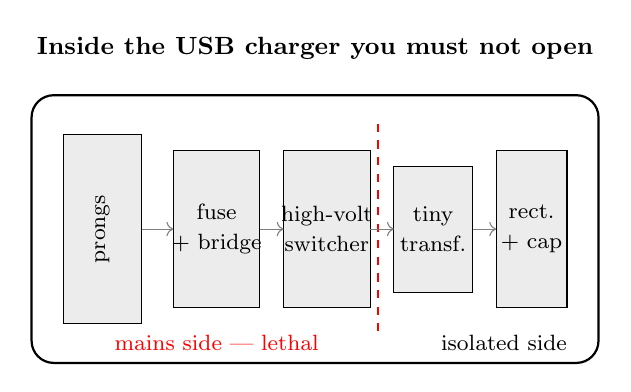
\begin{tikzpicture}[font=\small]
\draw[thick, rounded corners=8pt] (0,0) rectangle (7.2,3.4);
\node[align=center] at (3.6,4.0) {\textbf{Inside the USB charger you must not open}};
\draw[fill=gray!15] (0.4,0.5) rectangle (1.4,2.9); \node[rotate=90] at (0.9,1.7) {\footnotesize prongs};
\draw[fill=gray!15] (1.8,0.7) rectangle (2.9,2.7); \node[align=center] at (2.35,1.7) {\footnotesize fuse\\ \footnotesize + bridge};
\draw[fill=gray!15] (3.2,0.7) rectangle (4.3,2.7); \node[align=center] at (3.75,1.7) {\footnotesize high-volt\\ \footnotesize switcher};
\draw[fill=gray!15] (4.6,0.9) rectangle (5.6,2.5); \node[align=center] at (5.1,1.7) {\footnotesize tiny\\ \footnotesize transf.};
\draw[fill=gray!15] (5.9,0.7) rectangle (6.8,2.7); \node[align=center] at (6.35,1.7) {\footnotesize rect.\\ \footnotesize + cap};
\draw[dashed, thick, red] (4.4,0.4) -- (4.4,3.1);
\node[red, font=\footnotesize, align=center] at (2.35,0.25) {mains side --- lethal};
\node[font=\footnotesize, align=center] at (6.0,0.25) {isolated side};
\draw[->, gray] (1.4,1.7) -- (1.8,1.7); \draw[->, gray] (2.9,1.7) -- (3.2,1.7);
\draw[->, gray] (4.3,1.7) -- (4.6,1.7); \draw[->, gray] (5.6,1.7) -- (5.9,1.7);
\end{tikzpicture}

\caption{What is actually inside a \qty{5}{\volt} USB charger. Notice the
dashed line: everything left of it touches mains; the isolation boundary
is engineered, tested, and certified. Look — never open.}
\label{fig:wall}
\end{figure}

\begin{rulebox}[Mains: the hard boundary]
\begin{itemize}
\item \qty{230}{\volt} AC kills. It is not a bigger 9 V battery — a
mains shock across the chest can stop a heart, and a mains fault starts
fires, not sparks.
\item Never open, probe, repair, or re-use the inside of a wall
adapter, charger, or mains-powered brick — even unplugged, its
capacitors hold lethal charge for minutes.
\item Buy, don't build: USB supplies and lab bench supplies are
cheap, certified, and isolated. There is no beginner project whose
power stage should touch mains.
\item Cheap no-name chargers fail the isolation test too — buy known
brands from real shops.
\end{itemize}
\end{rulebox}

\begin{rulebox}[Battery energy: USB packs and LiPo]
USB power banks are the friendly face of lithium cells — that is why
they are allowed. The cells inside store real energy: shorted, a LiPo
sustains tens of amps and vents fire. Never pierce, crush, solder
directly on, or charge unattended loose lithium cells; use the
protected, cased packs as they come. A swollen pack is retired, not
``used up''.
\end{rulebox}

\section{Common mistakes}
\label{sec:mistakes07}

\begin{itemize}
\item \textbf{Applying the golden rules at the rails.} If the required
output exceeds the supply, the rules are already dead — check headroom
first (Section~\ref{sec:we-clip}).
\item \textbf{Forgetting decoupling capacitors.} An op-amp starved at
its supply pins oscillates mysteriously; \qty{100}{\nano\farad} across
the pins is cheap insurance, always.
\item \textbf{Using an op-amp as a comparator without hysteresis.} A
noisy input near the threshold chatters the output between rails; add
positive feedback or buy a real comparator.
\item \textbf{Expecting gain at any frequency.} GBW means a
$\times100$ amplifier is not one at \qty{100}{\kilo\hertz} — check the
bandwidth budget before the resistor ratio.
\item \textbf{Assuming the input range too.} Some parts read inputs
near the negative rail only; ``single-supply'' does not mean
``accepts any input''.
\end{itemize}

\section{Exercises}
\label{sec:exercises07}

\begin{exercise}[easy]
A buffer follows a sensor output of \qty{3.1}{\volt}. What is the
buffer's output voltage, and why would you bother if the number doesn't
change?
\end{exercise}

\begin{exercise}[easy]
An inverting amplifier has $R_{\mathrm{in}} = \qty{2}{\kilo\ohm}$,
$R_f = \qty{20}{\kilo\ohm}$. What is the gain, and what input gives
$+\qty{5}{\volt}$ out?
\end{exercise}

\begin{exercise}[easy]
A non-inverting amplifier needs gain $11$. If $R_2 = \qty{1}{\kilo\ohm}$,
choose $R_1$.
\end{exercise}

\begin{exercise}[easy]
Your op-amp is on $\pm\qty{9}{\volt}$ rails and saturates about
\qty{1.5}{\volt} inside them. You want a $\pm\qty{6}{\volt}$ sine out of
gain $20$. What is the largest input amplitude you can amplify cleanly?
\end{exercise}

\begin{exercise}[medium]
A comparator circuit has $R_1 = \qty{10}{\kilo\ohm}$ to ground and
$R_2 = \qty{30}{\kilo\ohm}$ to the output, which saturates at
$\pm\qty{10}{\volt}$. Find both switching thresholds $V_{T+}$ and
$V_{T-}$.
\end{exercise}

\begin{exercise}[medium]
Using $T = 2RC\ln\frac{1+k}{1-k}$: a relaxation oscillator runs at
\qty{250}{\hertz} with $k = 0.5$ and $C = \qty{100}{\nano\farad}$.
What is $R$?
\end{exercise}

\begin{exercise}[medium]
A project draws \qty{80}{\milli\ampere} at \qty{5}{\volt} and you can
feed the regulator \qty{9}{\volt}. Compare an LDO (dropout
\qty{0.4}{\volt}) against a buck module: which do you pick, and what
power does the loser waste? When would the answer flip?
\end{exercise}

\begin{exercise}[medium]
You need $\times50$ gain at \qty{20}{\kilo\hertz} from a
\qty{1}{\mega\hertz} GBW op-amp. Can you do it in one stage? What
open-loop gain does the chip actually offer there, and what does that
do to accuracy?
\end{exercise}

\begin{exercise}[hard]
(Implement) Extend \texttt{comparator\_osc.cir}: make $k \neq 0.5$ by
setting $R_1 = \qty{10}{\kilo\ohm}$, $R_2 = \qty{20}{\kilo\ohm}$
($k = \frac{1}{3}$). Derive the new predicted period, re-simulate, and
report measured vs predicted in a table. \textbf{Hint:}
$\ln\frac{1+k}{1-k} = \ln 2$ now.
\end{exercise}

\begin{exercise}[hard]
A \qty{12}{\volt}-to-\qty{5}{\volt} linear regulator supplies a
\qty{300}{\milli\ampere} load. Compute the dissipated power, and explain
why engineers choose a buck converter here — then explain when they
would \emph{not} (think noise, cost, battery standby).
\end{exercise}

\section{Summary}
\label{sec:summary07}

\begin{center}
\small
\begin{tabular}{@{}p{0.30\linewidth}p{0.62\linewidth}@{}}
\toprule
\textbf{Idea} & \textbf{One-line version} \\ \midrule
Golden rules & With negative feedback: inputs draw no current, and $v_+ = v_-$ — until the rails say otherwise. \\
Buffer & Copies a voltage without loading the source. \\
Inverting amp & Gain $-R_f/R_{\mathrm{in}}$; $v_-$ is a virtual ground. \\
Non-inverting amp & Gain $1 + R_1/R_2 \ge 1$; input sees no load. \\
Comparator & No taming feedback: output rails declare which input is bigger. \\
Hysteresis & Positive feedback gives two thresholds; noise can't dither the output. \\
Clipping & Demanded output beyond swing limit = flat-topped waveform. \\
Linear regulator & Burns the voltage difference as heat: simple, quiet, inefficient. \\
Switching regulator & Chops through an inductor: efficient, noisy. \\
USB supply & Pre-regulated, current-limited, safe — the book's bench supply. \\
Mains & \qty{230}{\volt} stays inside certified boxes. Buy, never build. \\
Decoupling & \qty{100}{\nano\farad} at every chip's supply pins, always. \\
\bottomrule
\end{tabular}
\end{center}

\section*{Notes}
\begin{enumerate}
\item \emph{All About Circuits}, vol.\ III, ch.\ 8 — the op-amp chapters
the buffer/inverting/comparator analyses follow~\cite{aacvol3}.
\item MIT \emph{6.002} lectures 8--12 (op-amp abstraction, negative
feedback) and 20+ (power) — the golden-rules framing and the honest
limits list~\cite{ocw6002}.
\item Horowitz \& Hill, \emph{The Art of Electronics} — the cited next
step for comparator subtleties, regulators, and real-world
op-amp pathologies~\cite{aoe}.
\end{enumerate}

\section*{Hints and answers}
\begin{description}
\item[Buffer (easy)] \qty{3.1}{\volt}. The point is the \emph{current}:
the buffer supplies load current from its rails while drawing $\sim 0$
from the sensor.
\item[Inverting gain (easy)] Gain $-10$; input $-\qty{0.5}{\volt}$.
\item[Non-inverting (easy)] $R_1 = \qty{10}{\kilo\ohm}$ ($1+10=11$).
\item[Headroom (easy)] Swing limit $\approx \pm 7.5$ V $>$ the
\qty{6}{\volt} needed; max clean input $= 6/20 = \qty{0.3}{\volt}$.
\item[Weak sensor (inline, \S\ref{sec:three})] Without buffer
$\approx \qty{0.227}{\volt}$; with buffer $\approx \qty{2.5}{\volt}$
--- the sim of \S\ref{sec:we-buffer} measures both.
\item[Mic gain (inline, \S\ref{sec:we-clip})] $R_f =
\qty{30}{\kilo\ohm}$, $R_{\mathrm{in}} = \qty{1}{\kilo\ohm}$;
$\pm 1.5$ V out is far inside the swing limit.
\item[Osc period (inline, \S\ref{sec:we-osc})] $RC = 1/(2\ln 3)\,
\mathrm{ms} \approx \qty{0.455}{\milli\second}$; e.g.\
$R = \qty{4.55}{\kilo\ohm}$, $C = \qty{100}{\nano\farad}$.
\item[Thresholds (medium)] $V_T = \frac{10}{40}\times 10 =
\pm\qty{2.5}{\volt}$: flips high at $+2.5$, low at $-2.5$.
\item[Oscillator $R$ (medium)] $R = \frac{1}{2fC\ln 3} \approx
\qty{18.2}{\kilo\ohm}$.
\item[LDO vs buck (medium)] LDO wastes $(9-5)\times 0.08 =
\qty{0.32}{\watt}$ with $4$ V of headroom $\gg$ \qty{0.4}{\volt}
dropout --- pick the LDO. Buck wins when current is amps, or battery
life beats noise.
\item[GBW (medium)] Open-loop gain at \qty{20}{\kilo\hertz} $\sim
10^{6}/2\times10^{4} = 50$ --- barely the wanted closed loop; split into
two $\times 7$ stages or choose a faster part.
\item[$k=1/3$ oscillator (hard)] $T = 2RC\ln 2 \approx
\qty{1.39}{\milli\second}$ predicted ($\approx\qty{721}{\hertz}$);
simulate and tabulate --- expect within $1\%$.
\item[Linear vs buck, \qty{300}{\milli\ampere} (hard)] $(12-5)\times
0.3 = \qty{2.1}{\watt}$ of heat --- buck territory. Skip it when noise
is critical, cost rules, or load is milliamps.
\end{description}

\chapter{Numbers, bits and Boolean algebra}
\label{ch:digital}

Every chapter so far treated voltage as a quantity — 0.227 volts here,
10.45 there. The digital world compresses all of that into two letters:
0 and 1. This chapter introduces the notation (binary, hex, two's
complement), the algebra that manipulates it (truth tables, De Morgan,
Karnaugh maps), and the first sight of a hardware description language —
a 20-line Verilog file that prints gate truth tables. After it, you will
be able to read a byte in any base, prove a simplification two different
ways, and turn an English sentence like ``the alarm sounds when the
ignition is on and the door is open or the belt is off'' into a minimal
gate network.

\section{Why two levels?}
\label{sec:twolevels}

Chapter 6's noise margins are the reason. A ``1'' is not
\qty{3.3}{\volt}; it is \emph{anything above} $V_{IH}$; a ``0'' is
anything below $V_{IL}$. The region between is forbidden — and the
margins $NM_L$, $NM_H$ budget how much noise a signal can pick up before
a receiver misreads it. Two levels, spaced far apart with a guard band,
is the cheapest possible error-correction scheme: any voltage that
drifts stays readable, and every gate regenerates the levels fresh.

\begin{checkpoint}[Two levels, one reason]
Binary is not a mathematical preference — it is the cheapest way to make
physical voltage carry information through noise. Keep asking of every
abstraction above it: \emph{what does a 1 physically mean here?}
\end{checkpoint}

\section{Binary, hex, and two's complement}
\label{sec:repr}

A byte is eight bits, and a number written $b_7b_6\ldots b_0$ means
$\sum_i b_i 2^i$. \emph{Hexadecimal}\index{hexadecimal} groups four bits
per digit (\texttt{0x00}--\texttt{0xFF}); the programmer's muscle memory
is knowing $2^4=16$, $2^8=256$, $2^{10}\approx10^{3}$ cold.

For negatives the convention is \emph{two's
complement}\index{two's complement}: the most significant bit carries
weight $-128$, not $+128$. So \texttt{0xFF} $= -1$, and the representable
range of a signed byte is $-128$ to $+127$ — asymmetric by one. The
payoff: \emph{no subtraction circuit is ever needed}; $a-b$ is just
$a+(\sim b + 1)$, and the same adder does both jobs.

\begin{exercise}[easy]
Write $-1$, $-128$, $+127$ in hex under two's complement; then compute
$100 - 50$ byte-wise without any subtraction: $100 + (\sim50 + 1)$.
\end{exercise}

\section{Truth tables}
\label{sec:tt}

A Boolean function of $n$ inputs has exactly $2^n$ input rows, and its
\emph{truth table}\index{truth table} is the complete enumeration — the
definition, not a summary. Everything later (K-maps, HDL testbenches)
re-arranges or re-prints this table; it is the ground truth.

Here is one in a new notation — \emph{Verilog}\index{Verilog}, the
hardware description language used from chapter 11 onward. You are not
expected to write this yet; read it with the numbered explanations in the
margin of your mind:

\begin{lstlisting}[caption={\ttfamily code/ch08\_gates\_tb.v --- a
behavioral truth printer. Every line explained below the output.},
label={lst:gatestb},abovecaptionskip=0pt]
// ch08_gates_tb.v -- behavioral gate truth printer
`timescale 1ns/1ps
module gates_tb;
  reg  a, b;            // inputs we sweep
  wire y_and, y_or, y_xor, y_nand, y_nor, y_xnor;

  assign y_and  = a & b;
  assign y_or   = a | b;
  assign y_xor  = a ^ b;
  assign y_nand = ~(a & b);
  assign y_nor  = ~(a | b);
  assign y_xnor = ~(a ^ b);

  integer i;
  initial begin
    $display("a b | AND OR XOR NAND NOR XNOR");
    $display("----+---------------------------------");
    for (i = 0; i < 4; i = i + 1) begin
      {a, b} = i[1:0];            // 00,01,10,11 in binary
      #1;
      $display("%b %b |  %b   %b   %b    %b    %b     %b",
               a, b, y_and, y_or, y_xor, y_nand, y_nor, y_xnor);
    end
    $finish;
  end
endmodule
\end{lstlisting}

\begin{lstlisting}[caption={Real output of
\texttt{iverilog -o gates\_tb ch08\_gates\_tb.v \&\& vvp gates\_tb}},
abovecaptionskip=0pt]
a b | AND OR XOR NAND NOR XNOR
----+---------------------------------
0 0 |  0   0   0    1    1     1
0 1 |  0   1   1    1    0     0
1 0 |  0   1   1    1    0     0
1 1 |  1   1   0    0    0     1
ch08_gates_tb.v:28: $finish called at 4000 (1ps)
\end{lstlisting}

Reading the file: \texttt{module}/\texttt{endmodule} wrap a circuit block;
\texttt{reg} holds values we set procedurally, \texttt{wire} is driven
continuously. \texttt{assign} makes a wire follow an expression
forever — that is the hardware, six gates drawn in text.
\texttt{initial ... begin ... end} runs once at simulation start (a
testbench block, not synthesizable). \texttt{\{a,b\}=i[1:0]} splits the
2-bit counter across two wires; \texttt{\#1} waits one tick;
\texttt{\$display} prints. The loop emits all $2^2=4$ rows — the truth
table, printed by the gates themselves.

The symbols for these gates are in Figure~\ref{fig:symbols}; the truth
table above is what each symbol means.

\begin{figure}[htbp]
\centering
% Gate symbols table (circuitikz logic ports, book palette)
\newcommand{\gatesym}[2]{%
  \begin{circuitikz}[baseline=(g.center), scale=0.75, transform shape]
    \node[#1] (g) {};
  \end{circuitikz} & #2 \\}
\begin{tabular}{@{}c l c l@{}}
AND ($ab$)   & \gatesym{american and port}{$y = a\cdot b$} &
NAND ($\overline{ab}$) & \gatesym{american nand port}{$y=\overline{a\cdot b}$} \\
OR ($a+b$)   & \gatesym{american or port}{$y = a+b$} &
NOR ($\overline{a+b}$) & \gatesym{american nor port}{$y=\overline{a+b}$} \\
XOR ($a\oplus b$) & \gatesym{american xor port}{$y = a\oplus b$} &
XNOR ($\overline{a\oplus b}$) & \gatesym{american xnor port}{$y=\overline{a\oplus b}$} \\
NOT ($\bar a$) & \gatesym{american not port}{$y=\bar a$} &
buffer & \gatesym{american buffer port}{$y=a$} \\
\end{tabular}

\caption{The seven gate symbols. Notice the small bubble on NAND, NOR,
XNOR, NOT: an output circle always means ``invert the plain version'' —
$\overline{AND}=NAND$, and so on.}
\label{fig:symbols}
\end{figure}

\begin{exercise}[medium]
From the printed table, write the Boolean expression for XNOR as a sum
of products of $a$, $b$, and their complements.
\end{exercise}

\section{De Morgan and the universal gates}
\label{sec:demorgan}

\begin{definition}[De Morgan's laws]
\index{De Morgan's laws}
\[
\overline{a\cdot b}=\bar a+\bar b,
\qquad
\overline{a+b}=\bar a\cdot\bar b.
\]
NOT distributes by \emph{swapping the operator}. Both directions are
provable by exhaustion — a truth table settles them in four rows.
\end{definition}

The payoff is practical: NAND alone can build every other gate
(Figure~\ref{fig:universal}), and so can NOR — either is a
\emph{universal gate}\index{universal gate}. Real silicon is made of
NANDs; De Morgan is why a designer can sketch in AND/OR and let the
synthesizer retarget to NAND/NOR without changing the function.

\begin{figure}[htbp]
\centering
% NAND universality: NOT, AND, OR from NANDs only
\begin{circuitikz}[american, scale=0.8, transform shape, font=\small]
% NOT from NAND (tie inputs)
\node[american nand port] (n1) at (0,0) {};
\draw (n1.in 1) -- (n1.in 2) to[short,-o] ++(-0.7,0) node[left] {$a$};
\draw (n1.out) to[short,-o] ++(0.4,0) node[right] {$\bar a$};
\node at (0,-1.4) {NOT};
% AND from NAND + NAND-NOT
\node[american nand port] (n2) at (3.4,0) {};
\node[american nand port] (n3) at (5.4,0) {};
\draw (n2.in 1) to[short,-o] ++(-0.7,0) node[left] {$a$};
\draw (n2.in 2) to[short,-o] ++(-0.7,0) node[left] {$b$};
\draw (n3.in 1) -- (n3.in 2);
\draw (n2.out) -- ++(0.6,0) |- (n3.in 1) -- ++(-0.6,0);
\draw (n3.out) to[short,-o] ++(0.4,0) node[right] {$ab$};
\node at (4.4,-1.4) {AND};
% OR from NAND-NOT inputs + NAND
\node[american nand port] (n4) at (8.0,0.5) {};
\node[american nand port] (n5) at (8.0,-0.9) {};
\node[american nand port] (n6) at (10.2,-0.2) {};
\draw (n4.in 1) -- (n4.in 2) to[short,-o] ++(-0.7,0) node[left] {$a$};
\draw (n5.in 1) -- (n5.in 2) to[short,-o] ++(-0.7,0) node[left] {$b$};
\draw (n4.out) -| (n6.in 1);
\draw (n5.out) -| (n6.in 2);
\draw (n6.out) to[short,-o] ++(0.4,0) node[right] {$a+b$};
\node at (9.0,-2.0) {OR (De Morgan)};
\end{circuitikz}

\caption{NAND building NOT, AND, and OR. Notice the OR shape: two
NAND-inverters feeding a NAND — that is De Morgan drawn in wires.}
\label{fig:universal}
\end{figure}

\begin{exercise}[medium]
Draw NOT, AND, and OR out of NOR gates only. (Hint: NOT is one NOR;
work through De Morgan.)
\end{exercise}

\section{Worked example 1: signed byte arithmetic, three ways}
\label{sec:we-bytes}

\textbf{Strategy.} Compute $45 - 83$ in an 8-bit byte three different
ways and watch them land on the same answer — that agreement is what
makes two's complement worth its asymmetry.

\textbf{Solution.}
\begin{enumerate}
\item \emph{Plain arithmetic}: $45-83=-38$. In signed hex,
$-38 = 256-38 = 218 = \texttt{0xDA}$.
\item \emph{Negate and add}: $-83$ is $\sim83+1 = \sim\texttt{0x53}+1 =
\texttt{0xAC}+1=\texttt{0xAD}$. Then $45+\texttt{0xAD} =
\texttt{0x2D}+\texttt{0xAD} = \texttt{0xDA}$ — the carry out of bit 7 is
discarded; the byte wraps and the answer is right.
\item \emph{Bit-check}: \texttt{0xDA} $=1101\,1010_2$: top bit $-128$ plus
$64+16+8+2=90$, total $-128+90=-38$. \checkmark
\end{enumerate}

The same adder did the subtraction; method 2 is literally what silicon
computes.

\section{Worked example 2: prove a simplification twice}
\label{sec:we-simp}

\textbf{Strategy.} Take $y = ab + a\bar b + \bar a b$. Prove it equals
$a+b$ first by exhaustion (truth table) then by algebra — the two proofs
compliment each other: the table is infallible but proves only this
instance; the algebra shows \emph{why} and generalizes.

\textbf{Solution.}
\begin{lstlisting}[caption={Truth-table check via
\texttt{ch08\_truth\_check.py} --- all 4 rows agree.},abovecaptionskip=0pt]
vars: A B
A B | A&B | A&~B | ~A&B   A|B
-----------------------------
0 0 |   0   0
0 1 |   1   1
1 0 |   1   1
1 1 |   1   1
EQUIVALENT on all 4 input rows
\end{lstlisting}

Algebraically: $ab + a\bar b = a(b+\bar b) = a$, so $y = a + \bar a b =
a + b$ (using $x + \bar x y = x + y$). Same conclusion, one line.

The checker used above is the book's truth-table tool — exercises will
meet it again:

\begin{lstlisting}[caption={\ttfamily code/ch08\_truth\_check.py ---
compares expressions exhaustively and prints every row.},
label={lst:tcheck},abovecaptionskip=0pt]
usage: python3 ch08_truth_check.py "I&D | I&~B" "I&(D|~B)"
# evaluates each expression on all 2^n input rows, prints the table,
# then EQUIVALENT or DIFFERENT with the first counterexample.
\end{lstlisting}

\section{Worked example 3: the alarm circuit}
\label{sec:we-alarm}

\textbf{Strategy.} ``The alarm buzzes when the ignition is on and either
the door is open or the seatbelt is unfastened.'' Name the inputs
$I, D, B$ (belt fastened = 1), write the truth table, reduce with a
K-map, then build three equivalent gate networks.

\textbf{Solution.} Rows where the alarm is off ($I=0$) are all zero;
when $I=1$, the alarm sounds for $D=1$ or $B=0$. The 3-variable K-map
(Figure~\ref{fig:kmap3}) groups two overlapping pairs:
$I\bar B$ and $ID$, giving
\[
y = I\cdot D + I\cdot\bar B = I\,(D+\bar B).
\]

\begin{lstlisting}[caption={Checker confirms the factored form
(verbatim).},abovecaptionskip=0pt]
vars: B D I
B D I | I&D | I&~B   I&(D|~B)
-----------------------------
0 0 0 |   0   0
0 0 1 |   1   1
0 1 0 |   0   0
0 1 1 |   1   1
1 0 0 |   0   0
1 0 1 |   0   0
1 1 0 |   0   0
1 1 1 |   1   1
EQUIVALENT on all 8 input rows
\end{lstlisting}

\begin{figure}[htbp]
\centering
% 3-var K-map for the alarm: I&D | I&~B -> I&D + I&~B
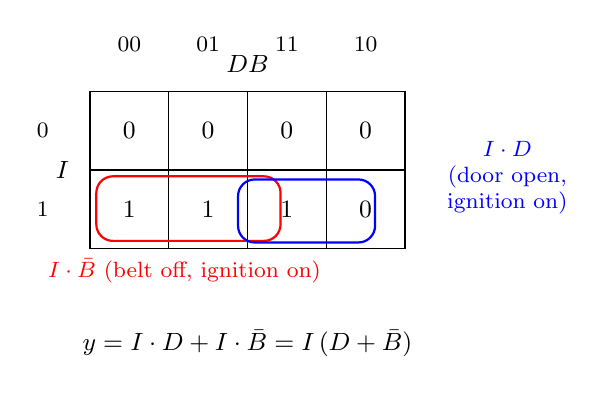
\begin{tikzpicture}[font=\small]
\draw[step=1] (0,0) grid (4,2);
\node at (-0.35,1.0) {$I$}; \node at (2.0,2.35) {$DB$};
\node[font=\footnotesize] at (-0.6,1.5) {0}; \node[font=\footnotesize] at (-0.6,0.5) {1};
\node[font=\footnotesize] at (0.5,2.6) {00}; \node[font=\footnotesize] at (1.5,2.6) {01};
\node[font=\footnotesize] at (2.5,2.6) {11}; \node[font=\footnotesize] at (3.5,2.6) {10};
% I row (bottom, I=1): DB cols 00->1, 01->1, 11->1, 10->0
\node at (0.5,0.5) {1}; \node at (1.5,0.5) {1}; \node at (2.5,0.5) {1}; \node at (3.5,0.5) {0};
\node at (0.5,1.5) {0}; \node at (1.5,1.5) {0}; \node at (2.5,1.5) {0}; \node at (3.5,1.5) {0};
\draw[red, thick, rounded corners=6pt] (0.08,0.10) rectangle (2.42,0.92);
\node[red, font=\footnotesize] at (1.2,-0.28) {$I\cdot\bar B$ (belt off, ignition on)};
\draw[blue, thick, rounded corners=6pt] (1.88,0.08) rectangle (3.62,0.88);
\node[blue, font=\footnotesize, align=center] at (5.3,0.9) {$I\cdot D$\\ (door open,\\ ignition on)};
\node at (2.0,-1.2) {$y = I\cdot D + I\cdot\bar B = I\,(D+\bar B)$};
\end{tikzpicture}

\caption{The alarm's 3-variable K-map. Notice the wrap: the $DB$ columns
run 00, 01, 11, 10 — a Gray-code order, so adjacent cells always differ
by exactly one bit; that is what makes groupings meaningful.}
\label{fig:kmap3}
\end{figure}

\begin{figure}[htbp]
\centering
% same function three ways: SOP AND-OR, factored, NAND-only
\begin{circuitikz}[american, scale=0.72, transform shape, font=\footnotesize]
% --- 1) AND-OR SOP: I&D + I&~B ---
\node[american not port] (nB) at (0.6,1.9) {};
\draw (nB.in) to[short,-o] ++(-0.5,0) node[left] {$B$};
\node[american and port] (a1) at (2.2,2.0) {};
\node[american and port] (a2) at (2.2,0.4) {};
\node[american or port] (o1) at (4.4,1.2) {};
\draw (nB.out) -| (a1.in 1);
\draw (a1.in 2) to[short,-o] ++(-1.9,0) node[left] {$I$};
\draw (a2.in 1) to[short,-o] ++(-1.9,0) node[left] {$I$};
\draw (a2.in 2) to[short,-o] ++(-1.9,0) node[left] {$D$};
\draw (a1.out) -| (o1.in 1); \draw (a2.out) -| (o1.in 2);
\draw (o1.out) to[short,-o] ++(0.5,0) node[right] {$y$};
\node at (2.6,-0.7) {$I\bar B + ID$};
% --- 2) factored: I(D + ~B) ---
\begin{scope}[xshift=7.2cm]
\node[american not port] (nB2) at (0.6,1.9) {};
\draw (nB2.in) to[short,-o] ++(-0.5,0) node[left] {$B$};
\node[american or port] (o2) at (2.2,1.2) {};
\node[american and port] (a3) at (4.4,0.9) {};
\draw (nB2.out) -| (o2.in 1);
\draw (o2.in 2) to[short,-o] ++(-1.9,0) node[left] {$D$};
\draw (a3.in 1) to[short,-o] ++(-0.9,0) node[left] {$I$};
\draw (o2.out) -| (a3.in 2);
\draw (a3.out) to[short,-o] ++(0.5,0) node[right] {$y$};
\node at (2.6,-0.7) {$I(D+\bar B)$};
\end{scope}
\end{circuitikz}
\vspace{4pt}
\begin{circuitikz}[american, scale=0.72, transform shape, font=\footnotesize]
% --- 3) NAND-only: ~( ~(I~B) * ~(ID) ) = (IB')' (ID)' then NAND them ---
\node[american not port] (nB3) at (0.6,1.9) {};
\draw (nB3.in) to[short,-o] ++(-0.5,0) node[left] {$B$};
\node[american nand port] (na) at (2.6,2.0) {};
\node[american nand port] (nb) at (2.6,0.4) {};
\node[american nand port] (nc) at (4.8,1.2) {};
\draw (nB3.out) -| (na.in 1);
\draw (na.in 2) to[short,-o] ++(-2.3,0) node[left] {$I$};
\draw (nb.in 1) to[short,-o] ++(-2.3,0) node[left] {$I$};
\draw (nb.in 2) to[short,-o] ++(-2.3,0) node[left] {$D$};
\draw (na.out) -| (nc.in 1); \draw (nb.out) -| (nc.in 2);
\draw (nc.out) to[short,-o] ++(0.5,0) node[right] {$y$};
\node at (2.8,-0.8) {NAND-only: $(I\bar B)' \cdot (ID)'$ NANDed};
\end{circuitikz}

\caption{The same alarm function three ways: sum-of-products, factored,
and NAND-only. The NAND version costs one more gate but uses a single
gate type — the trade real fabs make everywhere.}
\label{fig:threeways}
\end{figure}

\begin{exercise}[hard]
(Implement) The minimal form is $I\,(D+\bar B)$. Use the checker on
your machine to prove the sum-of-products and NAND-only forms agree on
all 8 rows; then decide which a fab would rather print.
\end{exercise}

\section{From expression to network}
\label{sec:pipeline}

The workflow this chapter just walked is a pipeline
(Figure~\ref{fig:pipeline}): sentence $\to$ truth table $\to$ K-map
$\to$ minimal sum-of-products $\to$ gate network. The same reduction a
synthesizer does in nanoseconds — learning to do it by hand is how you
\emph{audit} what the tool did, and why HDLBits drills (named in the
exercises) start at truth tables.

\begin{figure}[htbp]
\centering
% truth table -> K-map -> minimal expression pipeline
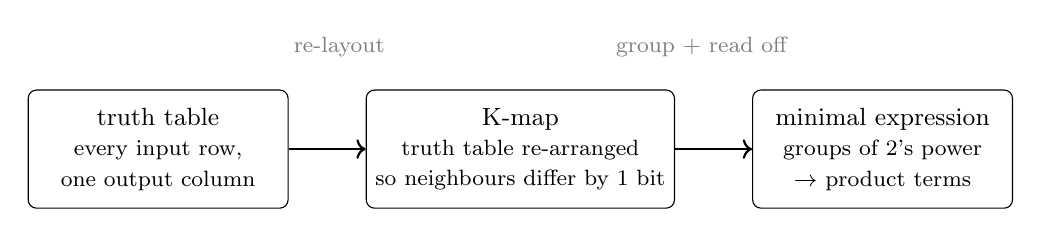
\begin{tikzpicture}[font=\small, box/.style={draw, rounded corners=3pt, align=center, minimum height=1.5cm, minimum width=3.3cm}]
\node[box] (tt) at (0,0) {truth table\\ \footnotesize every input row,\\ \footnotesize one output column};
\node[box] (km) at (4.6,0) {K-map\\ \footnotesize truth table re-arranged\\ \footnotesize so neighbours differ by 1 bit};
\node[box] (ex) at (9.2,0) {minimal expression\\ \footnotesize groups of 2's power\\ \footnotesize $\to$ product terms};
\draw[->, thick] (tt) -- (km);
\draw[->, thick] (km) -- (ex);
\node[font=\footnotesize, text=gray] at (2.3,1.3) {re-layout};
\node[font=\footnotesize, text=gray] at (6.9,1.3) {group + read off};
\end{tikzpicture}

\caption{The minimization pipeline. Notice which step is mechanical
(K-map re-layout is just a permutation of the truth table's rows) and
which step carries judgment (choosing the groups).}
\label{fig:pipeline}
\end{figure}

The 2-variable map of Figure~\ref{fig:kmap2} is the same picture,
smaller — the groups it draws are the exact terms of Worked Example 2.

\begin{figure}[htbp]
\centering
% 2-var K-map for AB + A~B + ~AB = A + B
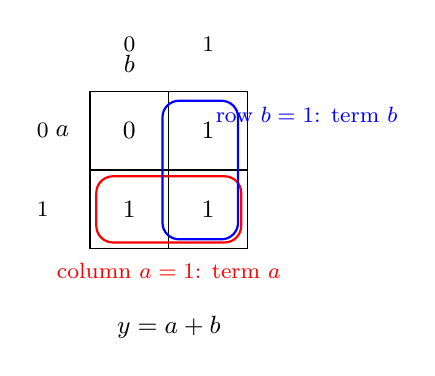
\begin{tikzpicture}[font=\small]
\draw[step=1] (0,0) grid (2,2);
\node at (-0.35,1.5) {$a$}; \node at (0.5,2.35) {$b$};
\node[font=\footnotesize] at (-0.6,1.5) {0}; \node[font=\footnotesize] at (-0.6,0.5) {1};
\node[font=\footnotesize] at (0.5,2.6) {0}; \node[font=\footnotesize] at (1.5,2.6) {1};
\node at (0.5,1.5) {0}; \node at (1.5,1.5) {1};
\node at (0.5,0.5) {1}; \node at (1.5,0.5) {1};
\draw[red, thick, rounded corners=6pt] (0.08,0.08) rectangle (1.92,0.92);
\node[red, font=\footnotesize] at (1.0,-0.28) {column $a=1$: term $a$};
\draw[blue, thick, rounded corners=6pt] (0.92,0.12) rectangle (1.88,1.88);
\node[blue, font=\footnotesize] at (2.75,1.7) {row $b=1$: term $b$};
\node at (1.0,-1.0) {$y = a + b$};
\end{tikzpicture}

\caption{The 2-variable K-map for $ab+a\bar b+\bar ab$: two groups of two
read off $a$ and $b$ directly.}
\label{fig:kmap2}
\end{figure}

\section{Common mistakes}
\label{sec:mistakes08}

\begin{itemize}
\item \textbf{Misreading place values} on multi-digit binary: read the
exponents, don't count digits — $10_2$ is two, not ten; \texttt{0x10} is
sixteen, not ``one-zero''.
\item \textbf{Sign slips in two's complement}: forgetting the top bit is
$-2^{n-1}$ gives wrong negatives; $\sim x$ alone is $-x-1$, not $-x$.
\item \textbf{Off-by-one on representable ranges}: a signed byte is
$-128\ldots+127$, asymmetric — you cannot negate $-128$ in 8 bits.
\item \textbf{Applying De Morgan halfway}: $\overline{ab}\ne\bar a\bar b$
— the operator must swap too.
\item \textbf{Thinking K-map adjacency is physical adjacency}: edges wrap
(left-right, top-bottom) because it's a torus, not a table.
\end{itemize}

\section{Exercises}
\label{sec:exercises08}

\begin{exercise}[easy]
Convert \texttt{0b10110010} to hex and decimal (unsigned) and to decimal
(signed).
\end{exercise}
\begin{exercise}[easy]
What is $-1 - 1$ in an 8-bit two's-complement byte? Show the hex.
\end{exercise}
\begin{exercise}[easy]
Write the truth table of $y=\bar a\bar b+\bar a b$. What common gate is it?
\end{exercise}
\begin{exercise}[easy]
Prove $\overline{a+b}=\bar a\bar b$ by exhaustion on all four input rows.
\end{exercise}
\begin{exercise}[medium]
Transform $\overline{\bar a + bc}$ into a product form without any
complement-of-a-sum remaining.
\end{exercise}
\begin{exercise}[medium]
Minimize $y = \bar a\bar b + a\bar b + ab$ and state the gate count
before and after.
\end{exercise}
\begin{exercise}[medium]
On paper, derive the alarm minimal form a second way: from the truth
table, write the full sum-of-products, then factor and absorb without a
K-map.
\end{exercise}
\begin{exercise}[medium]
In 8-bit two's complement, what is \texttt{0x7F + 1}? Name the
phenomenon.
\end{exercise}
\begin{exercise}[hard]
Design: a hallway light is on when (motion) or (dark and switch-on).
Derive minimal SOP from a truth table, then implement the truth
equivalence check in \texttt{ch08\_truth\_check.py} on the two forms.
Then do HDLBits ``Getting Started'' + the basic-gates set as external
drills.
\end{exercise}
\begin{exercise}[hard]
Prove XOR is also universal: build NOT, AND, OR from XOR + constants +
wires, or argue which one fails and why (this is a trick — one of them
cannot be built; identify which and say why).
\end{exercise}

\section{Summary}
\label{sec:summary08}

\begin{center}\small
\begin{tabular}{@{}p{0.32\linewidth}p{0.60\linewidth}@{}}
\toprule
\textbf{Idea} & \textbf{One-line version} \\ \midrule
Two levels & Cheapest noise immunity: wide rails + guard band. \\
Binary / hex & Place value $2^i$; hex = 4-bit shorthand. \\
Two's complement & Top bit weighs $-2^{n-1}$; adder subtracts free. \\
Truth table & The definition; $2^n$ rows is the whole function. \\
De Morgan & NOT distributes by swapping AND$\leftrightarrow$OR. \\
Universal gates & NAND alone, or NOR alone, builds everything. \\
K-map & Truth table re-laid so neighbours differ by one bit; groups of 2's power read off minimal SOP. \\
Synthesis & The pipeline sentence$\to$table$\to$map$\to$gates is what the tools automate. \\
\bottomrule
\end{tabular}
\end{center}

\section*{Notes}
\begin{enumerate}
\item \emph{All About Circuits}, Vol.~IV: Digital, ch.\ 1--8 — numerals,
Boolean algebra, gate properties, De Morgan, Karnaugh
maps~\cite{aacvol4}.
\item Harris \& Harris, \emph{Digital Design and Computer Architecture},
ch.\ 1--2 — chapter ordering and exercise style adapted
here~\cite{ddca}.
\end{enumerate}

\section*{Hints and answers}
\begin{description}
\item[Byte sign (easy)] \texttt{0xFF}=$-1$, \texttt{0x80}=$-128$,
\texttt{0x7F}=$+127$; $100+(\sim50+1)=100+206=306\to306-256=50$.
\item[XNOR SOP (medium)] $\bar a\bar b + ab$.
\item[NOR-only (medium)] NOT: tie inputs ($\overline{a+a}=\bar a$);
OR: one NOR ($\overline{a+b}$) inverted by NOR-NOT; AND: invert each
input with NOR-NOT, then NOR.
\item[Hex-dec (easy)] \texttt{0b10110010}=\texttt{0xB2}=178 unsigned,
$-78$ signed.
\item[Wrap (easy)] \texttt{0xFE}=$-2$.
\item[Gate ID (easy)] $\bar a$.
\item[De Morgan (easy)] Rows $00{:}1{=}1$; $01{:}0{=}0$; $10{:}0{=}0$;
$11{:}0{=}0$.
\item[Transform (medium)] $a\cdot\overline{bc}=a(\bar b+\bar c)$.
\item[Minimize (medium)] $y=\bar b+ab$ $\to$ then $\bar b+a$: 4 gates
$\to$ 1 (using $x+\bar xy=x+y$).
\item[Alarm, algebraic (medium)] $ID+I\bar B=I(D+\bar B)$ directly from
factoring; SOP full form collects the same three minterms.
\item[Overflow (medium)] \texttt{0x80} — signed overflow from $+127$ to
$-128$.
\item[Hallway (hard)] $y=M+DS$; verify both forms equivalent on all 8
rows; HDLBits drills build the same muscle in real HDL.
\item[XOR trick (hard)] AND cannot be built: XOR is affine —
every output is an XOR of inputs and constants, and AND is not affine.
\end{description}

\chapter{Combinational circuits}
\label{ch:comb}

Chapter 8 gave us the alphabet; this chapter builds the words.
Every useful digital circuit reduces to a handful of combinational
\emph{building blocks}\index{combinational logic} — multiplexers and
decoders route, adders and comparators compute, and all of them together
form the ALU at the heart of a CPU. After this chapter you will be able
to build a mux from gates and from \texttt{assign}, explain why a
ripple-carry adder is slow, decode a seven-segment display, and count
the speed/area trade in gate delays.

% from-zero:begin
\begin{rulebox}[Before you start]
Chapter~8 (Boolean algebra). \emph{Recap:} \emph{combinational} means the output depends only on the present inputs --- no memory.
\end{rulebox}
\begin{wins}[After this chapter you can]
\begin{itemize}
\item build a multiplexer and a decoder from gates;
\item build a ripple-carry adder and count its delay;
\item design a seven-segment decoder;
\item explain how these blocks become an ALU.
\end{itemize}
\end{wins}
\begin{principle}[How to think about this]
Combinational design is like building with plumbing: signals flow through, and the output simply reflects the input after a delay. The delay matters: a long chain of gates is slow, which is why the structure of an adder affects how fast a computer can run.
\end{principle}
% from-zero:end

\section{Multiplexers and decoders: the two routers}
\label{sec:routers}

A \emph{multiplexer}\index{multiplexer} (mux) selects one of $2^n$ inputs
according to $n$ select lines: $y = d_{s}$. Built from gates it is a
2-level sum-of-products — a decoder of $s$ feeding ANDs whose outputs
OR together. Its dual, the \emph{decoder}\index{decoder}, spreads one
enable into $2^n$ mutually-exclusive lines: $y_i = e \cdot [s=i]$.
Together they are the routers of combinational logic — mux chooses a
path, decoder chooses a destination.

\begin{exercise}[easy]
Write the sum-of-products for a 2:1 mux in terms of $s, d_0, d_1$; then
show it collapses to $\bar s d_0 + s d_1$.
\end{exercise}

\begin{figure}[htbp]
\centering
% 4:1 mux tree from three 2:1 muxes (rectangle muxes for clarity)
\begin{tikzpicture}[font=\footnotesize,
  mux/.style={draw, minimum width=1.4cm, minimum height=1.0cm}]
\node[mux] (m1) at (0,1.2) {};
\node[mux] (m2) at (0,-0.4) {};
\node[mux] (m3) at (3,0.4) {};
\draw[->] (-2.0,1.6) node[left] {$d_0$} -- (m1.west |- -0,1.6);
\draw[->] (-2.0,0.8) node[left] {$d_1$} -- (m1.west |- -0,0.8);
\draw[->] (-2.0,0.0) node[left] {$d_2$} -- (m2.west |- -0,0.0);
\draw[->] (-2.0,-0.8) node[left] {$d_3$} -- (m2.west |- -0,-0.8);
\node[right, font=\scriptsize] at (m1.east) {};
\draw[->] (m1.east) -- ++(0.6,0) |- ($(m3.west)+(0,0.25)$);
\draw[->] (m2.east) -- ++(0.6,0) |- ($(m3.west)+(0,-0.25)$);
\node[above, font=\scriptsize] at ($(m3.west)+(0,0.25)$) {};
\draw[->] (0,-1.7) node[below] {$s_0$} -- (0,-0.9) |- (m1.south);
\draw[->] (m2.south) ++(0,-0.6) -- (m2.south);
\draw[->] (3,-1.4) node[below] {$s_1$} -- (m3.south);
\draw[->] (m3.east) -- ++(0.5,0) node[right] {$y$};
\end{tikzpicture}

\caption{A 4:1 mux as a tree of three 2:1 muxes. Notice the select fanout:
$s_0$ picks inside the leaves, $s_1$ picks between them — the same
address-decoding pattern repeats all the way up to memory chips.}
\label{fig:muxtree}
\end{figure}

\section{Worked example 1: a 4:1 mux, gates then \texttt{assign}}
\label{sec:we-mux}

\textbf{Strategy.} Build it twice — once as a gate tree so the cost is
visible, once as a one-line \texttt{assign} so the intent is — and
convince ourselves the synthesizer sees them as the same circuit.

\textbf{Solution.} As gates, Figure~\ref{fig:muxtree}: three 2:1 muxes,
2 levels of logic, $s_0$ at the leaves, $s_1$ at the root. In Verilog it
collapses to a single selection:
\begin{lstlisting}[caption={The same 4:1 mux as one \texttt{assign}
--- read-only here; toolchain formalised in ch11.},abovecaptionskip=0pt]
assign y = s1 ? (s0 ? d3 : d2) : (s0 ? d1 : d0);
\end{lstlisting}
The ternary nest reads exactly like the tree: top-level \texttt{s1?}
chooses a branch, each \texttt{s0?} chooses a leaf. Synthesis maps both
descriptions to the same lookup table; the \texttt{assign} version wins
because it says \emph{what} and leaves the \emph{how} to the tool.

\section{Adders: half, full, and ripple-carry}
\label{sec:adders}

A \emph{half adder}\index{half adder} adds two bits: $s=a\oplus b$,
$c=ab$ — an XOR and an AND. A \emph{full adder}\index{full adder} adds
three (two operands plus carry-in):
$s=a\oplus b\oplus c_{in}$ and $c_{out}=ab+c_{in}(a\oplus b)$ — two XORs,
two ANDs, an OR (Figure~\ref{fig:fulladder}).

\begin{figure}[htbp]
\centering
% full adder gate map: sum = a^b^cin ; cout = ab + cin(a^b)
\begin{circuitikz}[american, scale=0.75, transform shape, font=\footnotesize]
\node[american xor port] (x1) at (0,2.0) {};
\node[american xor port] (x2) at (2.4,1.7) {};
\node[american and port] (a1) at (0.6,0.0) {};
\node[american and port] (a2) at (2.4,0.4) {};
\node[american or port]  (o1) at (4.4,0.6) {};
\draw (x1.in 1) to[short,-o] ++(-0.9,0) node[left] {$a$};
\draw (x1.in 2) to[short,-o] ++(-0.9,0) node[left] {$b$};
\draw (x1.out) -| (x2.in 1);
\draw (x2.in 2) to[short,-o] ++(-2.6,0) node[left] {$c_{in}$};
\draw (x2.out) to[short,-o] ++(0.5,0) node[right] {sum};
\draw (a1.in 1) to[short,-o] ++(-1.5,0) node[left] {$a$};
\draw (a1.in 2) to[short,-o] ++(-1.5,0) node[left] {$b$};
\draw (a1.out) -| (o1.in 2);
\draw (x1.out) ++(0.4,0) -- ++(0,-0.9) -| (a2.in 1);
\draw (x2.in 2) ++(-0.4,0) -- ++(0,-1.0) -| (a2.in 2);
\draw (a2.out) -| (o1.in 1);
\draw (o1.out) to[short,-o] ++(0.4,0) node[right] {$c_{out}$};
\end{circuitikz}

\caption{Full-adder gate map. Notice the shared $a\oplus b$ feeding both
the sum XOR and the carry AND — reusing a partial result is the whole
trick, and why the gate count is 5 not 7.}
\label{fig:fulladder}
\end{figure}

\begin{lstlisting}[caption={\ttfamily code/ch09\_full\_adder.v --- the
cell the ripple reuses.},label={lst:fa},abovecaptionskip=0pt]
module full_adder(a, b, cin, sum, cout);
  input  a, b, cin;
  output sum, cout;
  assign sum  = a ^ b ^ cin;
  assign cout = (a & b) | (cin & (a ^ b));
endmodule
\end{lstlisting}

Chaining four cells gives the \emph{ripple-carry
adder}\index{ripple-carry adder} of Figure~\ref{fig:ripple}: each carry
must \emph{settle} before the next full adder can even start — the carry
\emph{ripples} through.

\begin{figure}[htbp]
\centering
% 4-bit ripple carry annotated with propagation delay
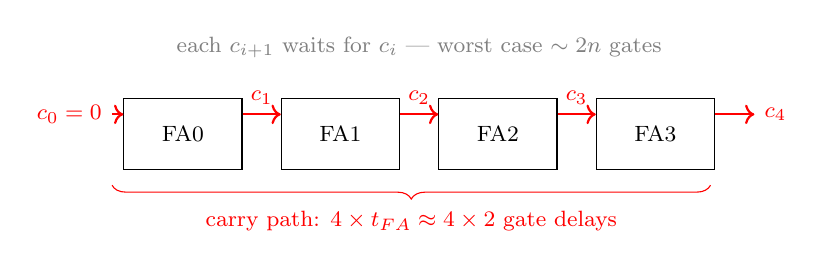
\begin{tikzpicture}[font=\footnotesize, cell/.style={draw, minimum width=1.5cm, minimum height=0.9cm}]
\node[cell] (f0) at (0,0) {FA0};
\node[cell] (f1) at (2,0) {FA1};
\node[cell] (f2) at (4,0) {FA2};
\node[cell] (f3) at (6,0) {FA3};
\draw[->, red, thick] (-0.9,0.25) node[left] {$c_0=0$} -- (f0.west|-0,0.25);
\draw[->, red, thick] (f0.east|-0,0.25) -- node[above] {$c_1$} (f1.west|-0,0.25);
\draw[->, red, thick] (f1.east|-0,0.25) -- node[above] {$c_2$} (f2.west|-0,0.25);
\draw[->, red, thick] (f2.east|-0,0.25) -- node[above] {$c_3$} (f3.west|-0,0.25);
\draw[->, red, thick] (f3.east|-0,0.25) -- ++(0.5,0) node[right] {$c_4$};
\draw[red, decorate, decoration={brace, mirror, amplitude=5pt}] (-0.9,-0.65) -- (6.7,-0.65)
  node[midway, below=6pt] {carry path: $4\times t_{FA}\approx 4\times 2$ gate delays};
\node[gray] at (3,1.1) {each $c_{i+1}$ waits for $c_i$ — worst case $\sim2n$ gates};
\end{tikzpicture}

\caption{The ripple carry chain. Notice what is \emph{not} parallel:
$c_4$ is a function of every bit upstream, so the worst-case delay grows
with $n$, not with the answer's size.}
\label{fig:ripple}
\end{figure}

\begin{lstlisting}[caption={\ttfamily code/ch09\_adder4.v + its
testbench --- the 4-cell chain, exercised.},label={lst:adder4},abovecaptionskip=0pt]
module adder4(a, b, sum, cout);
  input  [3:0] a, b;
  output [3:0] sum;
  output       cout;
  wire [2:0]   c;
  full_adder fa0(.a(a[0]), .b(b[0]), .cin(1'b0),  .sum(sum[0]), .cout(c[0]));
  full_adder fa1(.a(a[1]), .b(b[1]), .cin(c[0]),  .sum(sum[1]), .cout(c[1]));
  full_adder fa2(.a(a[2]), .b(b[2]), .cin(c[1]),  .sum(sum[2]), .cout(c[2]));
  full_adder fa3(.a(a[3]), .b(b[3]), .cin(c[2]),  .sum(sum[3]), .cout(cout));
endmodule
\end{lstlisting}

\begin{lstlisting}[caption={Last rows of the real \texttt{vvp} output ---
carry out asserted at 15+5, 15+10, 15+15.},abovecaptionskip=0pt]
 a +  b = (cout,sum)
15 + 10 = (1, 9)
15 + 15 = (1,14)
ch09_adder4_tb.v:16: $finish called at 64000 (1ps)
\end{lstlisting}

\section{Worked example 2: counting the delay}
\label{sec:we-delay}

\textbf{Strategy.} Estimate the ripple's worst-case delay honestly, then
compare a 2-level (sum-of-products) alternative — and see why the trade
is speed \emph{vs} area, not free lunch.

\textbf{Solution.} Each full adder's carry-out is 2 gate-delays after its
carry-in settles (XOR then AND-OR). For a 4-bit ripple the carry walks
$4\times 2=8$ levels; for $n$ bits, $\approx 2n$. The alternative —
compute carry directly as a 2-level function of all $2n$ inputs — needs
$2^n$ product terms per carry: $n=8$ needs 256 AND gates per carry
versus 8 FAs. Figure~\ref{fig:adderblock} sketches the real compromise
(carry-lookahead, built properly later): more logic in exchange for a
bounded $\sim$4-level path. The lesson is the \emph{trade itself}: in
combinational design there is almost always a faster circuit if you are
willing to pay for it in gates.

\begin{figure}[htbp]
\centering
% adder block diagram, CLA teaser
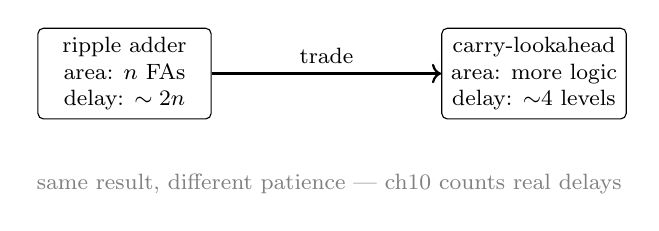
\begin{tikzpicture}[font=\footnotesize, box/.style={draw, rounded corners=2pt, minimum width=2.2cm, minimum height=1.0cm, align=center}]
\node[box] (rc) at (0,0) {ripple adder\\ area: $n$ FAs\\ delay: $\sim2n$};
\node[box] (cla) at (5.2,0) {carry-lookahead\\ area: more logic\\ delay: $\sim$4 levels};
\draw[->, thick] (rc) -- (cla) node[midway, above] {trade};
\node[gray] at (2.6,-1.4) {same result, different patience — ch10 counts real delays};
\end{tikzpicture}

\caption{Speed-vs-area in one picture. Notice both blocks produce the
same sum — only the \emph{path length} to it differs.}
\label{fig:adderblock}
\end{figure}

\begin{exercise}[medium]
An 8-bit ripple adder is roughly $2\times$ a 4-bit's delay and $8\times$
the two-level carry logic's area. Write the delay for $n=16$ and the
product-term count for the 2-level $c_{16}$ alternative.
\end{exercise}

\section{Comparators, encoders, priority}
\label{sec:priority}

A \emph{comparator}\index{comparator (digital)} is a subtractor that
keeps only the sign: equality is an XNOR tree, magnitude falls out of
the borrow chain. An \emph{encoder}\index{encoder} runs a decoder
backwards — $2^n$ lines in, $n$ bits out — and a \emph{priority
encoder} resolves ties by position, which is exactly what an interrupt
controller does: \texttt{casez} with wildcard rows, don't-cares marking
``lower priority does not matter.''

\textbf{Don't-cares}\index{don't-care} are a contract, not an omission:
writing \texttt{x} on impossible inputs lets the minimizer pick the
cheaper neighbor — but only for inputs the rest of the system truly
never produces.

\section{Worked example 3: seven-segment decoder}
\label{sec:we-seg7}

\textbf{Strategy.} A digit $\to$ 7 segments is just 7 Boolean functions
of 4 inputs. Write the truth table once (rows 10--15 as don't-cares),
minimize each segment, then let a \texttt{case} statement say it plainly
and the simulator print the check.

\textbf{Solution.} The segment map is Figure~\ref{fig:seg7map}; the
decoder and its \texttt{case}:

\begin{lstlisting}[caption={\ttfamily code/ch09\_seg7.v --- BCD to
cathodes \texttt{\{a,b,c,d,e,f,g\}}.},label={lst:seg7},abovecaptionskip=0pt]
module seg7(d, seg);
  input  [3:0] d;
  output reg [6:0] seg;
  always @(*) begin
    case (d)
      4'd0: seg = 7'b1111110;
      4'd1: seg = 7'b0110000;
      4'd2: seg = 7'b1101101;
      4'd3: seg = 7'b1111001;
      4'd4: seg = 7'b0110011;
      4'd5: seg = 7'b1011011;
      4'd6: seg = 7'b1011111;
      4'd7: seg = 7'b1110000;
      4'd8: seg = 7'b1111111;
      4'd9: seg = 7'b1111011;
      default: seg = 7'b0000000;
    endcase
  end
endmodule
\end{lstlisting}

\begin{lstlisting}[caption={Real truth-dump of
\texttt{ch09\_seg7\_tb.v} --- digits 0--9 plus the don't-care rows.},abovecaptionskip=0pt]
 d | abcdefg
---+--------
 0 | 1111110
 1 | 0110000
 2 | 1101101
 3 | 1111001
 4 | 0110011
 5 | 1011011
 6 | 1011111
 7 | 1110000
 8 | 1111111
 9 | 1111011
10 | 0000000
...
15 | 0000000
\end{lstlisting}

The \texttt{default} is the don't-care policy made concrete: rows the
driver never produces get \texttt{x} on paper and \texttt{0000000} here —
the display dark rather than arbitrary.

\begin{figure}[htbp]
\centering
% seven-segment letter map + seg-e example cells
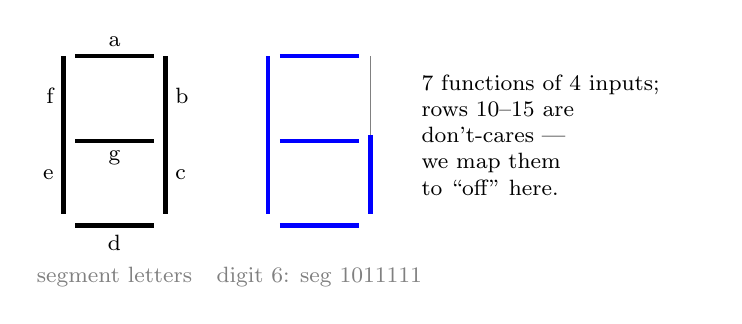
\begin{tikzpicture}[font=\footnotesize]
% segment map
\draw[ultra thick] (0,2) -- (1,2); \node[above] at (0.5,2) {a};
\draw[ultra thick] (1.15,1) -- (1.15,2); \node[right] at (1.15,1.5) {b};
\draw[ultra thick] (1.15,0) -- (1.15,1); \node[right] at (1.15,0.5) {c};
\draw[ultra thick] (0,-0.15) -- (1,-0.15); \node[below] at (0.5,-0.15) {d};
\draw[ultra thick] (-0.15,0) -- (-0.15,1); \node[left] at (-0.15,0.5) {e};
\draw[ultra thick] (-0.15,1) -- (-0.15,2); \node[left] at (-0.15,1.5) {f};
\draw[ultra thick] (0,0.92) -- (1,0.92); \node[below] at (0.5,0.92) {g};
\node[gray] at (0.5,-0.8) {segment letters};
% lit shape for digit 6 (a f g e d c on, b off)
\begin{scope}[xshift=2.6cm]
\draw[ultra thick, blue] (0,2) -- (1,2);
\draw[thin, gray] (1.15,1) -- (1.15,2);
\draw[ultra thick, blue] (1.15,0) -- (1.15,1);
\draw[ultra thick, blue] (0,-0.15) -- (1,-0.15);
\draw[ultra thick, blue] (-0.15,0) -- (-0.15,1);
\draw[ultra thick, blue] (-0.15,1) -- (-0.15,2);
\draw[ultra thick, blue] (0,0.92) -- (1,0.92);
\node[gray] at (0.5,-0.8) {digit 6: seg 1011111};
\end{scope}
% don't-care policy note
\begin{scope}[xshift=6.2cm]
\node[align=left, text width=3.6cm] at (0,1.0)
 {7 functions of 4 inputs;\\ rows 10--15 are\\ don't-cares —\\ we map them\\ to ``off'' here.};
\end{scope}
\end{tikzpicture}

\caption{Segment letters and the digit-6 pattern. Notice each of the
seven bars is an independent function of the same 4 inputs — seven small
K-maps, not one big one.}
\label{fig:seg7map}
\end{figure}

\begin{exercise}[medium]
Rows 10--15 were don't-cares. If a bug drives them with \texttt{1010},
what does our \texttt{default} show? What would a cheaper minimizer
exploiting the don't-cares legally show instead?
\end{exercise}

\section{The ALU preview and the road to a bus}
\label{sec:alu}

Stack these blocks: mux to pick the operation, adder to add, comparator
to compare, and you have the shape of an \emph{ALU}\index{ALU}
(Figure~\ref{fig:alu}) — the combinational heart of the chapter-14 CPU.
The last step is wiring: bundle the same-width wires and call the bundle
a \emph{bus}\index{bus} — a single line on the diagram that is really
$w$ bits wide. Everything later (registers, memories, datapaths) speaks
in buses; combinational logic speaks in bits.

\begin{figure}[htbp]
\centering
% ALU symbol preview
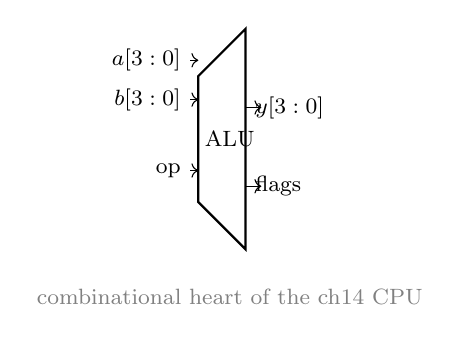
\begin{tikzpicture}[font=\footnotesize]
\draw[thick] (0,0) -- (0,1.6) -- (0.6,2.2) -- (0.6,-0.6) -- cycle;
\node at (0.4,0.8) {ALU};
\node[left] at (-0.1,1.8) {$a[3:0]$}; \draw[->] (-0.1,1.8) -- (0,1.8);
\node[left] at (-0.1,1.3) {$b[3:0]$}; \draw[->] (-0.1,1.3) -- (0,1.3);
\node[left] at (-0.1,0.4) {op}; \draw[->] (-0.1,0.4) -- (0,0.4);
\node[right] at (0.6,1.2) {$y[3:0]$}; \draw[->] (0.6,1.2) -- (0.8,1.2);
\node[right] at (0.6,0.2) {flags}; \draw[->] (0.6,0.2) -- (0.8,0.2);
\node[gray] at (0.4,-1.2) {combinational heart of the ch14 CPU};
\end{tikzpicture}

\caption{The ALU as a symbol. Notice it is pure combination: data in,
result out — no memory. The \texttt{flags} output is just comparators'
results bundled out for later chapters to use.}
\label{fig:alu}
\end{figure}

\section{Common mistakes}
\label{sec:mistakes09}

\begin{itemize}
\item \textbf{K-map adjacency slips}: the edges wrap — top touches
bottom, left touches right. A group of 4 that is not a rectangle is not
a group.
\item \textbf{Incomplete truth tables}: a missing row is not a 0; feed
the minimizer all $2^n$ rows or it will ``minimize'' a lie.
\item \textbf{Treating don't-cares as values}: \texttt{x} means
``whatever is cheapest,'' not ``0'' — if the input can actually occur,
it was never a don't-care.
\item \textbf{Forgetting \texttt{default}} in a \texttt{case}: unlisted
rows leave wires undriven and synthesize latches, not logic.
\item \textbf{Confusing encoder and decoder direction}: decoder spreads
one code to many lines; encoder packs many lines to one code.
\end{itemize}

\section{Exercises}
\label{sec:exercises09}

\begin{exercise}[easy]
Write the 4:1 mux truth table for $d_0..d_3$ and $s_1s_0$; how many rows?
\end{exercise}
\begin{exercise}[easy]
Half-adder: show $s=a\oplus b$ and $c=ab$ from the truth table.
\end{exercise}
\begin{exercise}[easy]
What does a 3-to-8 decoder output when $s=101$, $e=1$? When $e=0$?
\end{exercise}
\begin{exercise}[easy]
In our ripple chain, why does $c_4$'s delay not depend on the data
pattern? When does it?
\end{exercise}
\begin{exercise}[medium]
Design a 4:2 priority encoder: inputs $i_0..i_3$ (highest first),
output the index of the highest asserted bit plus a valid flag. Write
the truth table using don't-cares.
\end{exercise}
\begin{exercise}[medium]
Show a subtractor is ``an adder plus two's complement'': write
$y=a-b$ as $a+\bar b+1$ in gates, reusing the adder4 structure.
\end{exercise}
\begin{exercise}[medium]
Estimate how many LUTs (a 4-input truth table each) a function of 6
inputs needs in the worst case, and how many if it factors neatly.
\end{exercise}
\begin{exercise}[medium]
Seven-seg segment $e$ is on for digits $\{0,2,6,8\}$. Using rows 10--15
as don't-cares, minimize $e$ on paper.
\end{exercise}
\begin{exercise}[hard]
(Implement) Extend \texttt{ch09\_adder4\_tb.v} to drive all $16^2$ pairs
and assert \texttt{cout,sum == a+b} each row; run it and report.
\end{exercise}
\begin{exercise}[hard]
A comparator: write the 2-bit-magnitude comparison $a>b$ as a Boolean
expression, then show it equals ``subtract and check the borrow.''
\end{exercise}

\section{Summary}
\label{sec:summary09}

\begin{center}\small
\begin{tabular}{@{}p{0.30\linewidth}p{0.62\linewidth}@{}}
\toprule
\textbf{Block} & \textbf{One-line version} \\ \midrule
Mux & Data selects which input passes; decoder's dual. \\
Decoder & One enable, $2^n$ mutually-exclusive lines. \\
Half / full adder & XOR+AND, then XOR chain + carry-merge; the cell. \\
Ripple carry & $n$ FAs chained; worst delay $\sim 2n$ levels. \\
Two-level carry & $\sim$4 levels but $2^n$ terms — speed bought with area. \\
Comparator & A subtractor read for sign only. \\
Priority encoder & ``First wins'': \texttt{casez} + don't-cares. \\
Seven-seg decoder & Seven 4-input functions sharing one truth table. \\
ALU & Mux + adder + comparator = the combinational CPU heart. \\
\bottomrule
\end{tabular}
\end{center}

\section*{Notes}
\begin{enumerate}
\item Harris \& Harris, \emph{Digital Design and Computer Architecture},
ch.\ 2, 5 — mux/decoder structure, adder taxonomy~\cite{ddca}.
\item \emph{All About Circuits}, Vol.~IV: Digital — combinational
building blocks~\cite{aacvol4}.
\item \emph{fpga4fun.com} — small complete FPGA projects, the book's
``one project per concept'' model~\cite{fpga4fun}.
\end{enumerate}

\section*{Hints and answers}
\begin{description}
\item[2:1 mux (easy)] $y=\bar s d_0 + s d_1$ — decoder of $s$ feeding
ANDs into an OR, the universal 2-level shape.
\item[16-bit delay (medium)] $\approx 2n=32$ levels ripple vs
$\sim 2^{16}$ terms for a flat $c_{16}$ — the trade explodes, so lookahead
splits the difference.
\item[Default policy (medium)] \texttt{1010} $\to$ \texttt{0000000} —
dark. A minimizer using the \texttt{x} rows could legally show
anything; it owes correctness only on rows 0--9.
\item[4:1 table (easy)] 4 select states $\times$ don't-care data = 16
rows enumerated.
\item[Half adder (easy)] $s=1$ iff $a\ne b$; $c=1$ iff $a=b=1$.
\item[Decoder (easy)] $s=101,e=1$: line 5 high; $e=0$: all zero.
\item[Ripple delay (easy)] Worst case is data-independent (carry must
propagate end-to-end); average case depends on the operands.
\item[Priority encoder (medium)] Rows like \texttt{1---} $\to$ index 0
when $i_0=1$ regardless of the rest.
\item[Subtractor (medium)] Invert $b$, set $c_0=1$: one inverter row
plus the same chain — the adder computes $a+(\bar b+1)$.
\item[LUTs (medium)] Naive $2^6=64$ rows on 4-input LUTs; a factored
function can be a handful — structure matters more than input count.
\item[Segment $e$ (medium)] $e = \bar d_0\,(\bar d_2 + d_1)$ — two
groups of four, exploiting three \texttt{x} cells.
\item[Exhaustive tb (hard)] Loop \texttt{a} 0--15, \texttt{b} 0--15,
compare \texttt{\{cout,sum\}} to \texttt{a+b}; 256 rows, all pass.
\item[Comparator (hard)] $a>b$: $a_1\bar b_1 +
(a_1 \odot b_1)\,a_0\bar b_0$ with $\odot$ XNOR — equivalently, the
borrow out of $a-b$.
\end{description}

\chapter{Sequential circuits and state machines}
\label{ch:seq}

Chapter 9's circuits were \emph{memoryless}: same inputs, same outputs,
forever. Real machines need to \emph{remember} — which is what a bank
account, a traffic light, and a CPU register have in common. This
chapter introduces feedback (latches and flip-flops), registers and
counters, and the finite state machine; the running simulation shows
the classic latch bug that silently ships when the two are confused.
After it, you will be able to design a small FSM end to end and know why
every button that talks to a clock needs two flops.

\section{Feedback and memory}
\label{sec:feedback}

Wire a gate's output back toward its input and the circuit gains
\emph{state}\index{state}. Two cross-coupled NORs form the SR
\emph{latch}\index{SR latch} — the first memory: $S=1$ sets, $R=1$
resets, both 0 holds. Add an enable input and you get the D
\emph{latch}\index{D latch}: while \texttt{en} is high, $q$ follows
$d$; while low, it holds. \emph{Transparent} is the operative word —
the output can change whenever the enable is up, not just at a tick.

The \emph{D flip-flop}\index{D flip-flop} trades transparency for a
shutter: $q$ samples $d$ \emph{only} on the rising clock edge
(\texttt{posedge}). Level vs edge is the difference between a window
and a photograph — and the difference between a circuit that follows
glitches and one that ignores them.

\section{Worked example 1: the latch bug, live}
\label{sec:we-latch}

\textbf{Strategy.} Drive a latch and a flip-flop with the same
\texttt{d}, open the latch's \texttt{en} for one window with a glitch
inside, and watch who follows the glitch.

\textbf{Solution.} Two cells:
\begin{lstlisting}[caption={\ttfamily code/ch10\_dff.v --- latch vs
flip-flop, same inputs.},label={lst:dff},abovecaptionskip=0pt]
module d_latch(en, d, q);
  input en, d;
  output reg q;
  always @(*) if (en) q = d;      // follows d while en=1
endmodule
module d_ff(clk, d, q);
  input clk, d;
  output reg q;
  always @(posedge clk) q <= d;   // samples d only at clk rise
endmodule
\end{lstlisting}

\begin{lstlisting}[caption={Excerpt of the real \texttt{vvp} run ---
the latch tracks the mid-window glitch; the FF waits for an edge.},
abovecaptionskip=0pt]
t= 12 en=1 clk=0 d=0 | latch=0 ff=1
t= 15 en=1 clk=1 d=0 | latch=0 ff=0
t= 16 en=1 clk=1 d=1 | latch=1 ff=0
t= 25 en=0 clk=1 d=1 | latch=1 ff=1
\end{lstlisting}

At t=12 the input glitched low and the latch fell in step — the FF did
not notice (its edge was not due). At t=16 the latch snapped to the new
\texttt{d} mid-cycle; the FF held its old sample until t=25, the next
rising edge. Figure~\ref{fig:timing} is the same data as waveforms.

\begin{figure}[htbp]
\centering
% latch vs FF timing, real VCD data (ch10_dff_timing.dat)
\begin{tikzpicture}
\begin{axis}[width=12.8cm, height=6.6cm,
  xlabel={time (ns)}, xmin=0, xmax=42,
  ylabel={level}, ymin=-0.4, ymax=5.6, ytick=\empty,
  legend cell align=left, legend style={font=\scriptsize, at={(0.5,-0.16)}, anchor=north, legend columns=5},
  axis lines=left]
\addplot[const plot, thick, gray]   table[x=t,y=clk]   {figures/ch10/ch10_dff_timing.dat}; \addlegendentry{clk}
\addplot[const plot, thick, ink]    table[x=t,y expr=\thisrow{en}+1.1] {figures/ch10/ch10_dff_timing.dat}; \addlegendentry{en}
\addplot[const plot, thick, accent] table[x=t,y expr=\thisrow{d}+2.2]  {figures/ch10/ch10_dff_timing.dat}; \addlegendentry{d}
\addplot[const plot, thick, red]    table[x=t,y expr=\thisrow{latch}+3.3] {figures/ch10/ch10_dff_timing.dat}; \addlegendentry{latch q}
\addplot[const plot, thick, blue]   table[x=t,y expr=\thisrow{ff}+4.4]   {figures/ch10/ch10_dff_timing.dat}; \addlegendentry{ff q}
\draw[dashed, red] (axis cs:12,0) -- (axis cs:12,4.0) node[font=\scriptsize, above, align=center] {glitch\\followed};
\draw[dashed, blue] (axis cs:25,0) -- (axis cs:25,5.4) node[font=\scriptsize, above, align=center] {edge\\samples};
\end{axis}
\end{tikzpicture}

\caption{Latch vs flip-flop, real simulated traces. Notice the latch's
\emph{window}: inside it, every wiggle on \texttt{d} reaches \texttt{q}.
The FF changes only at clock edges — one sample, then done.}
\label{fig:timing}
\end{figure}

That is why synchronous design uses edge-triggered flops everywhere:
the edge gives the whole machine a heartbeat and lets every block's
output settle into registers before the next beat.

\begin{exercise}[medium]
In the trace, \texttt{en} went high at t=8 and low at t=21, while the
clock ran all along. State precisely which \texttt{d} values the FF
sampled at t=5, 15, 25, and why the latch's \texttt{q} differs at t=16.
\end{exercise}

\section{Setup, hold, registers, buses}
\label{sec:setup}

For the edge sample to be meaningful, \texttt{d} must be stable a
little \emph{before} the edge (\emph{setup
time}\index{setup time}) and a little \emph{after} (\emph{hold
time}\index{hold time}) — the analysis of those windows is Book 7's
job; here the concept matters: the clock edge is a contract, and
combinational delays are how you budget it.

A \emph{register}\index{register} is a row of flip-flops clocked
together — Figure~\ref{fig:register}; a \emph{bus} is the bundle of
wires feeding and leaving registers.

\begin{figure}[htbp]
\centering
% register + bus diagram
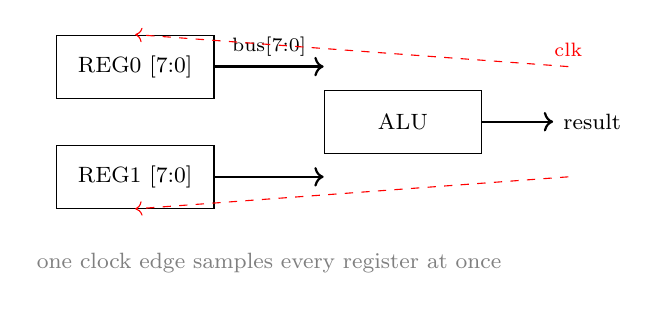
\begin{tikzpicture}[font=\footnotesize, reg/.style={draw, minimum width=2.0cm, minimum height=0.8cm}]
\node[reg] (r0) at (0,0) {REG0 [7:0]};
\node[reg] (r1) at (0,-1.4) {REG1 [7:0]};
\node[reg] (alu) at (3.4,-0.7) {ALU};
\draw[->, thick] (r0.east) -- node[above, font=\scriptsize] {bus[7:0]} (alu.west |- r0.east);
\draw[->, thick] (r1.east) -- (alu.west |- r1.east);
\draw[->, thick] (alu.east) -- ++(0.9,0) node[right] {result};
\draw[->, dashed, red] (5.5,0) node[above, font=\scriptsize] {clk} -- (r0.north);
\draw[->, dashed, red] (5.5,-1.4) -- (r1.south);
\node[gray] at (1.7,-2.5) {one clock edge samples every register at once};
\end{tikzpicture}

\caption{Registers around an ALU. Notice the same \texttt{clk} fans
out to every register — one edge, every value sampled simultaneously;
between edges the combinational ALU settles.}
\label{fig:register}
\end{figure}

\section{Counters}
\label{sec:counters}

A \emph{counter}\index{counter} is a register that adds 1 per edge.
Ripple counters chain toggle flip-flops (Figure~\ref{fig:counter});
synchronous counters compute \texttt{q+1} in parallel — the useful
ones add \texttt{en} (only count when told) and a terminal-count flag.

\begin{figure}[htbp]
\centering
% counter structure
\begin{tikzpicture}[font=\footnotesize, cell/.style={draw, minimum width=1.3cm, minimum height=0.8cm}]
\node[cell] (t0) at (0,0) {TFF0};
\node[cell] (t1) at (1.9,0) {TFF1};
\node[cell] (t2) at (3.8,0) {TFF2};
\node[cell] (t3) at (5.7,0) {TFF3};
\draw[->, red, thick] (-1,0) node[left] {clk} -- (t0.west);
\draw[->, thick] (t0.east) -- node[above, font=\scriptsize] {$q_0$} (t1.west);
\draw[->, thick] (t1.east) -- node[above, font=\scriptsize] {$q_1$} (t2.west);
\draw[->, thick] (t2.east) -- node[above, font=\scriptsize] {$q_2$} (t3.west);
\draw[->, thick] (t3.east) -- ++(0.5,0) node[right, font=\scriptsize] {$q_3$};
\draw[->, ink] (0,-0.8) node[left] {en} -- ++(0.4,0) |- (t0.south);
\node[gray] at (2.8,-1.7) {each T flip-flop toggles only when all lower bits are 1};
\end{tikzpicture}

\caption{Counter structure. Notice each stage toggles only when every
lower bit is 1 — counting is carry-propagation made visible.}
\label{fig:counter}
\end{figure}

\begin{lstlisting}[caption={\ttfamily code/ch10\_counter.v ---
enable + terminal count.},label={lst:counter},abovecaptionskip=0pt]
module counter(clk, en, q, tc);
  input clk, en;
  output reg [3:0] q = 0;
  output tc;
  assign tc = (q == 4'd15) & en;
  always @(posedge clk)
    if (en) q <= q + 1;
endmodule
\end{lstlisting}

\begin{lstlisting}[caption={Real run tail --- rollover at 15 with
\texttt{tc} asserted, counting resumes from 0.},abovecaptionskip=0pt]
t=155 en=1 | q=15 tc=1
t=165 en=1 | q= 0 tc=0
t=175 en=1 | q= 1 tc=0
\end{lstlisting}

\section{Worked example 2: a 1 Hz tick from 27 MHz}
\label{sec:we-tick}

\textbf{Strategy.} The Tang Nano 9K board's oscillator runs at 27 MHz;
blinking an LED at 1 Hz needs a prescaler that counts
$27\,000\,000$ cycles, then toggles — a counter with a terminal count
wired to an output flip.

\textbf{Solution.} $\log_2(27{\times}10^6)\approx 24.7$, so a 25-bit
counter suffices. Count to $13\,500\,000$, reset, toggle the blink:
$13.5{\times}10^6$ ticks per half-second. In Verilog the whole prescaler
is one \texttt{if} inside the \texttt{always} block plus an output flip —
the same \texttt{counter} pattern at scale. The honest check: the LED
pin needs only the toggle — the count is internal state, exactly what
registers are for.

\section{Finite state machines}
\label{sec:fsm}

An \emph{FSM}\index{finite state machine} is states + edges + outputs:
a register holding the state, combinational next-state logic, and
output logic. \emph{Moore}\index{Moore machine} outputs depend on state
only; \emph{Mealy}\index{Mealy machine} outputs also take the inputs
directly (Figure~\ref{fig:mealy_moore}). The disciplined three-block
style — one \texttt{always} per job — keeps the machine readable and
the synthesizer honest.

\begin{figure}[htbp]
\centering
% Mealy vs Moore templates
\begin{tikzpicture}[font=\footnotesize,
  box/.style={draw, rounded corners=2pt, minimum width=2.4cm, minimum height=1.1cm, align=center}]
\node[box] (regm) at (0,2.4) {state\\ register};
\node[box] (nxtm) at (3.8,2.4) {next-state\\ logic};
\node[box] (outm) at (3.8,0.4) {output logic\\ Moore: f(state)};
\draw[->, thick] (-1.8,2.4) node[left] {in} -- (nxtm.west);
\draw[->, thick] (regm.east) -- (nxtm.west);
\draw[->, thick] (regm.east) |- (outm.west);
\draw[->, thick] (outm.east) -- ++(0.8,0) node[right] {out};
\draw[->, thick] (nxtm.south) |- (regm.north);
% mealy path
\draw[->, thick, accent, dashed] (-1.8,2.4) ++(0,-0.15) .. controls (1,1.1) .. (outm.west)
  node[midway, above, font=\scriptsize, accent] {Mealy: inputs reach output directly};
\end{tikzpicture}

\caption{Moore vs Mealy. Notice the dashed path: only Mealy lets inputs
reach the output within the same cycle — one edge faster, one glitch
path wider.}
\label{fig:mealy_moore}
\end{figure}

\section{Worked example 3: the traffic-light FSM, end to end}
\label{sec:we-traffic}

\textbf{Strategy.} State diagram first (Figure~\ref{fig:fsm}), then an
encoding, then the three-block Verilog, then the simulator prints the
cycle for us to check against the diagram.

\textbf{Solution.} Four states — NS green, NS yellow, EW green, EW
yellow — each transition on a timer:

\begin{figure}[htbp]
\centering
% traffic FSM state diagram (Moore)
\begin{tikzpicture}[font=\footnotesize, state/.style={draw, circle, minimum size=1.9cm, align=center, inner sep=1pt}]
\node[state] (g1) at (0,0) {NS\_G\\ \scriptsize NS=grn, EW=red};
\node[state] (y1) at (3.4,0) {NS\_Y\\ \scriptsize NS=ylw, EW=red};
\node[state] (g2) at (3.4,-3.0) {EW\_G\\ \scriptsize EW=grn, NS=red};
\node[state] (y2) at (0,-3.0) {EW\_Y\\ \scriptsize EW=ylw, NS=red};
\draw[->, thick] (g1) -- node[above] {timer} (y1);
\draw[->, thick] (y1) -- node[right] {timer} (g2);
\draw[->, thick] (g2) -- node[below] {timer} (y2);
\draw[->, thick] (y2) -- node[left] {timer} (g1);
\draw[->, dashed, ink] (-1.4,1.4) node[left] {rst} -- (g1.north west);
\end{tikzpicture}

\caption{The traffic machine. Notice outputs ride \emph{inside} the
states (Moore): NS is green only in \texttt{NS\_G}, full stop.}
\label{fig:fsm}
\end{figure}

\begin{lstlisting}[caption={\ttfamily code/ch10\_traffic\_fsm.v ---
always-three-block style.},label={lst:fsm},abovecaptionskip=0pt]
module traffic_fsm(clk, rst, ns, ew);
  input clk, rst;
  output reg [1:0] ns, ew;
  localparam NS_G=2'd0, NS_Y=2'd1, EW_G=2'd2, EW_Y=2'd3;
  reg [1:0] state = NS_G, nxt;
  always @(*) begin
    case (state)
      NS_G: nxt = NS_Y;  NS_Y: nxt = EW_G;
      EW_G: nxt = EW_Y;  EW_Y: nxt = NS_G;
      default: nxt = NS_G;
    endcase
  end
  always @(posedge clk) state <= rst ? NS_G : nxt;
  always @(*) begin
    ns = (state==NS_G) ? 2'b00 : (state==NS_Y) ? 2'b01 : 2'b10;
    ew = (state==EW_G) ? 2'b00 : (state==EW_Y) ? 2'b01 : 2'b10;
  end
endmodule
\end{lstlisting}

\begin{lstlisting}[caption={The real full-cycle trace --- GRN
(\texttt{00})$\to$YEL (\texttt{01}) around the loop, EW red
(\texttt{10}) throughout the NS phase.},abovecaptionskip=0pt]
t= 15 rst=0 state=0 | NS=00 EW=10
t= 25 rst=0 state=1 | NS=01 EW=10
t= 35 rst=0 state=2 | NS=10 EW=00
t= 45 rst=0 state=3 | NS=10 EW=01
t= 55 rst=0 state=0 | NS=00 EW=10
\end{lstlisting}

The printed cycle matches the diagram edge-for-edge: NS goes green,
yellow, then EW green, yellow, and back — Moore outputs change only
when the state does.

\begin{exercise}[medium]
Extend the machine with a pedestrian-wait state entered from
\texttt{NS\_G} only when a button input is high. Which block changes —
next-state, register, or output?
\end{exercise}


\section{Worked example 4: Mealy answers a cycle early}
\label{sec:we-mealy}

\textbf{Strategy.} Give the same rising edge to a Moore detector and a
Mealy detector and watch the outputs disagree by exactly one cycle —
the price and prize of reading inputs at the output.

\textbf{Solution.}
\begin{lstlisting}[caption={\ttfamily code/ch10\_mm\_tb.v run ---
\texttt{mealy=1} at t=15, the cycle the edge lands;
\texttt{moore=1} waits for t=25.},abovecaptionskip=0pt]
t=  5 x=0 | mealy=0 moore=0
t= 15 x=1 | mealy=1 moore=0
t= 25 x=1 | mealy=0 moore=1
t= 35 x=0 | mealy=0 moore=1
\end{lstlisting}

Mealy's output is combinational on the input, so it fires \emph{in} the
edge's cycle — one cycle faster, and one glitch-path wider (a mid-cycle
wiggle on \texttt{x} would reach \texttt{yme} too). Moore's rides the
state, always a registered answer. Rule of thumb: outputs that must be
clean (LED, motor, write-enable) go Moore; outputs that must be quick
(requests, acknowledges) can pay the Mealy price.

\section{Worked example 5: the ``101'' detector, end to end}
\label{sec:we-seq101}

\textbf{Strategy.} The second classic FSM: detect \texttt{101} on a
serial input \emph{with overlap} (a found ``1'' may start the next
pattern). Four states, then let the sim find both hits in
\texttt{11010110}.

\textbf{Solution.}
\begin{lstlisting}[caption={\ttfamily code/ch10\_seq101.v --- the
overlap lives in \texttt{FOUND}'s edges.},label={lst:seq101},abovecaptionskip=0pt]
module seq101(clk, x, hit);
  input clk, x; output reg hit;
  localparam IDLE=0, GOT1=1, GOT10=2, FOUND=3;
  reg [1:0] st = IDLE, nx;
  always @(*) case (st)
    IDLE:  nx = x ? GOT1 : IDLE;
    GOT1:  nx = x ? GOT1 : GOT10;
    GOT10: nx = x ? FOUND : IDLE;
    FOUND: nx = x ? GOT1 : GOT10;   // overlap: the 1 restarts
    default: nx = IDLE;
  endcase
  always @(posedge clk) st <= nx;
  always @(*) hit = (st == FOUND);
endmodule
\end{lstlisting}

\begin{lstlisting}[caption={Real run over \texttt{11010110} --- hits at
t=45 and t=65, the second riding the first's last bit.},abovecaptionskip=0pt]
t= 35 x=1 state=2 hit=0
t= 45 x=0 state=3 hit=1
t= 55 x=1 state=2 hit=0
t= 65 x=1 state=3 hit=1
t= 75 x=0 state=1 hit=0
\end{lstlisting}

The overlap is the \texttt{FOUND} row: on \texttt{x=1} we go to
\texttt{GOT1}, not \texttt{IDLE} — that 1 was both the end of one
pattern and the start of the next. One line of the transition table
carries the whole ``with overlap'' requirement.

\section{Metastability and the two-flop rule}
\label{sec:meta}

One honest paragraph: a flip-flop whose input changes exactly at the
edge does not pick 0 or 1 — it can sit \emph{between} them, and may
stay undecided for an unbounded (but exponentially unlikely) time.
That \emph{metastability}\index{metastability} is physics, not a bug.
The defense is Figure~\ref{fig:sync}: run every asynchronous input
through \emph{two} flops — the first absorbs the rare bad sample, the
second sees only settled logic. \textbf{Never clock a button into
logic without the synchroniser}; every switch in later chapters goes
through this shape.

\begin{figure}[htbp]
\centering
% two-flop synchroniser
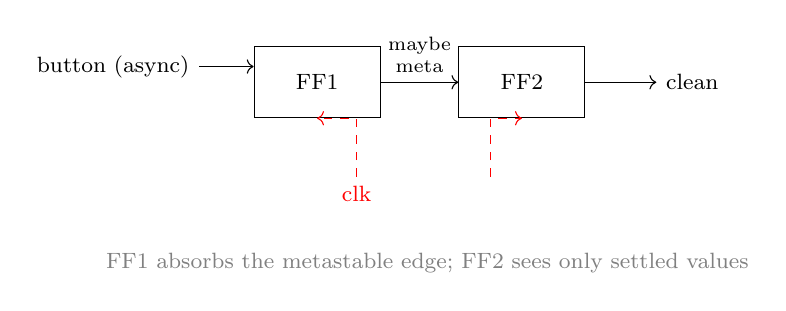
\begin{tikzpicture}[font=\footnotesize, cell/.style={draw, minimum width=1.6cm, minimum height=0.9cm}]
\node[cell] (f1) at (0,0) {FF1};
\node[cell] (f2) at (2.6,0) {FF2};
\draw[->] (-1.5,0.2) node[left] {button (async)} -- (f1.west |- 0,0.2);
\draw[->] (f1.east) -- node[above, font=\scriptsize, align=center] {maybe\\meta} (f2.west);
\draw[->] (f2.east) -- ++(0.9,0) node[right] {clean};
\draw[->, dashed, red] (0.5,-1.2) node[below] {clk} |- (f1.south);
\draw[->, dashed, red] (2.2,-1.2) |- (f2.south);
\node[gray] at (1.4,-2.3) {FF1 absorbs the metastable edge; FF2 sees only settled values};
\end{tikzpicture}

\caption{The two-flop synchroniser. Notice what is \emph{not} there:
no guarantee FF1 settles — only that FF2's input is one whole cycle
older, which settles the probability to negligible.}
\label{fig:sync}
\end{figure}

\section{Common mistakes}
\label{sec:mistakes}

\begin{itemize}
\item \textbf{Latch vs flip-flop confusion}: \texttt{@(*)} on
everything infers transparency and follows glitches — default to
\texttt{posedge} always.
\item \textbf{Incomplete sensitivity lists}: a \texttt{case} without
\texttt{default} leaves the output undriven on unlisted states and
invents a latch you never drew.
\item \textbf{Unreachable states}: an encoding wider than needed
leaves ghost states; route every default back somewhere real.
\item \textbf{Blocking vs nonblocking}: in clocked blocks use
\texttt{<=}; mixing is the classic silent-race source.
\item \textbf{Async inputs to logic}: skipping the two-flop
synchroniser on a button works 99.9\% of the time — and fails on the
demo day.
\end{itemize}

\section{Exercises}
\label{sec:exercises}

\begin{exercise}[easy]
Level vs edge: name the behavior each device exhibits and the Verilog
edge keyword for each.
\end{exercise}
\begin{exercise}[easy]
A 3-bit counter starting at 5: what are the next four counts?
\end{exercise}
\begin{exercise}[easy]
Which block of the three holds memory? Which two are pure combination?
\end{exercise}
\begin{exercise}[easy]
Why does Moore timing lag Mealy by up to a cycle?
\end{exercise}
\begin{exercise}[medium]
Pattern detector: FSM over bits detecting \texttt{101} with overlap.
Draw the states.
\end{exercise}
\begin{exercise}[medium]
Gray counter: why is Gray encoding safer for cross-domain sampling of
a count?
\end{exercise}
\begin{exercise}[medium]
The forgotten \texttt{else}: \texttt{if (en) q <= d;} inside
\texttt{@(*)} — what does the synthesizer build and why is it wrong?
\end{exercise}
\begin{exercise}[medium]
Prescaler: give the count value and bit width to get 10 Hz from 27 MHz.
\end{exercise}
\begin{exercise}[hard]
(Implement) Write \texttt{traffic\_tb} that asserts the exact state
cycle and count a violation; then add a walk-light state.
\end{exercise}
\begin{exercise}[hard]
A vending machine takes only 5- and 10-rupiah coins, dispenses at 15:
draw the FSM, encode it, and argue Moore vs Mealy.
\end{exercise}

\begin{exercise}[easy]
An SR latch with NOR gates: which inputs set, reset, and hold — and what
forbidden input pair breaks the abstraction?
\end{exercise}
\begin{exercise}[medium]
Register file: sketch two 8-bit registers and one shared bus; who decides
which register drives the bus, and what gate shape does it?
\end{exercise}
\begin{exercise}[medium]
Latency count: in the mm\_tb run, how many clock cycles separate the
first \texttt{mealy=1} from the last \texttt{moore=1}? Explain both.
\end{exercise}
\begin{exercise}[medium]
One-hot vs binary: our traffic machine used 2 bits for 4 states. Give
the one-hot encoding, its gate-count intuition, and when it wins.
\end{exercise}
\begin{exercise}[medium]
Serial adder: two numbers arrive one bit-pair per cycle. Draw the 2-state
FSM that outputs their sum (hint: one bit of state is a carry register —
you already built the combinational part in ch9).
\end{exercise}
\begin{exercise}[hard]
Design a debounced-button FSM: button $\to$ two-flop sync $\to$
edge-detect $\to$ one clean pulse per press, however long the press.
State the states.
\end{exercise}

\section{Summary}
\label{sec:summary}

\begin{center}\small
\begin{tabular}{@{}p{0.30\linewidth}p{0.62\linewidth}@{}}
\toprule
\textbf{Idea} & \textbf{One-line version} \\ \midrule
Latch & Transparent window — follows inputs while enabled. \\
Flip-flop & Photograph at the edge — the heartbeat's shutter. \\
Setup/hold & The edge contract; Book 7 does the math. \\
Register/bus & Edge-sampled row + the wires that feed it. \\
Counter & A register that adds 1 — \texttt{en} makes it a prescaler. \\
FSM (3 blocks) & State reg + next-state + output; never mix them. \\
Moore vs Mealy & State-only vs input-to-output path (1 cycle). \\
Metastability & Physics of the edge; sync it with two flops, always. \\
\bottomrule
\end{tabular}
\end{center}


\section*{Further reading}
\begin{itemize}
\item Harris \& Harris, \emph{Digital Design and Computer Architecture},
2nd ed., ch.\ 3 --- the reference for latch/FF discipline and FSM style;
free companion materials at \url{pages.hmc.edu/harris/ddca/}
(undergraduate level; the chapter's primary source~\cite{ddca}).
\item Kuphaldt, \emph{All About Circuits} Vol.\ IV (Digital),
sequential chapters --- alternative prose walk-through of the same
ladder; free textbook~\cite{aacvol4}.
\item MIT OCW \emph{6.004 Computation Structures} (2017) ---
university-level sequential logic lectures and labs, course page on
\url{ocw.mit.edu}
(undergraduate level; the academic version of this chapter).
\item Nisan \& Schocken, \emph{nand2tetris.org/course} project 3
(Memory) --- build the same registers bottom-up from DFFs in their HDL
(intro level; a second implementation of the same ideas).
\item HDLBits, \texttt{hdlbits.01xz.net} --- the Circuits/Sequential
problem set: small self-checking FSM drills named in the exercises
(practice engine, free).
\item \emph{fpga4fun.com} --- short real FPGA projects that consume
exactly these primitives (project ideas, intermediate).
\end{itemize}

\begin{rulebox}[Watch instead]
\begin{itemize}
\item \emph{Building an 8-bit breadboard computer} (full playlist),
Ben Eater, $\sim$20 videos --- the register/counter/FSM concepts here
built physically on breadboards; matches \S\ref{sec:feedback},
\S\ref{sec:setup}, \S\ref{sec:counters}. Accessed 2026-10-11.
\item \emph{D flip-flop} (single video), Ben Eater, $\sim$15 min ---
the DFF built from gates in front of you; matches
\S\ref{sec:feedback}--\S\ref{sec:we-latch}. Accessed 2026-10-11.
\end{itemize}
\end{rulebox}

\section*{Notes}
\begin{enumerate}
\item Harris \& Harris, \emph{Digital Design and Computer Architecture},
ch.\ 3 — latches, flops, FSM style~\cite{ddca}.
\item \emph{All About Circuits}, Vol.~IV: Digital — sequential
building blocks~\cite{aacvol4}.
\item HDLBits problem sets — the FSM drills named in the
exercises~\cite{hdlbits}.
\end{enumerate}

\section*{Hints and answers}
\begin{description}
\item[Trace (medium)] FF samples $d$ at t=5 (=1), 15 (=0), 25 (=1);
the latch passed the t=16 value mid-window, the FF waited to t=25.
\item[Pedestrian (medium)] Next-state logic + encoding only; outputs
ride on the states (Moore).
\item[Level/edge (easy)] Latch: level, \texttt{@(*)}; FF: edge,
\texttt{posedge clk}.
\item[3-bit count (easy)] 5,6,7,0,1.
\item[Blocks (easy)] The state register; next-state and output are
combinational.
\item[Moore lag (easy)] Outputs settle only after the state advances.
\item[101 detector (medium)] 4 states (none/1/10/101); on completion
input 0 sends you back for overlap.
\item[Gray (medium)] Only one bit flips per step — an async sample
can be off by at most one count.
\item[Missing else (medium)] Unassigned paths infer a latch holding
\texttt{q} — an invisible memory you never drew.
\item[10 Hz prescaler (medium)] $1.35{\times}10^6$ ticks per
half-period, 21 bits.
\item[Walk light (hard)] One more state + a \texttt{walk} input; the
tb's cycle assertion catches any skipped state.
\item[Vending (hard)] 4 states (0/5/10/dispense); Moore keeps the
dispense output glitch-free.
\item[SR latch (easy)] S=1 sets, R=1 resets, both 0 holds; S=R=1 is the
forbidden pair (output depends on release order).
\item[Register file (medium)] An enable line per register picks the
driver; each output goes through a mux or tri-state buffer.
\item[Latency count (medium)] t=15 to t=35: two edges — Mealy fires in
the sample's own cycle, Moore only after the state advances.
\item[One-hot (medium)] 4 bits, one hot per state; next-state logic is
one AND-OR row per destination — wins when speed beats area and $n$
is small.
\item[Serial adder (medium)] 2 states C=0/C=1 (the carry); each cycle
outputs $a_i\oplus b_i\oplus C$ and stores the new carry.
\item[Debounce (hard)] States idle/pressed/wait-release + a settling
counter; pulse out on the synced edge only.
\end{description}

\backmatter
\begin{thebibliography}{99}
\bibitem{sannemo2025} J.~Sannemo, \emph{Principles of Algorithmic Problem Solving}, 2025. \url{https://usaco.guide/PAPS1.pdf}
\bibitem{aacvol1} T.~R. Kuphaldt, \emph{Lessons in Electric Circuits}, Vol.~I: DC, 5th ed. (minor revisions 2021--2023). Free under the Design Science License. \url{https://www.allaboutcircuits.com/textbook/direct-current/}
\bibitem{aacvol3} T.~R. Kuphaldt, \emph{Lessons in Electric Circuits}, Vol.~III: Semiconductors, 5th ed. \url{https://www.allaboutcircuits.com/textbook/semiconductors/}
\bibitem{aacvol4} T.~R. Kuphaldt, \emph{Lessons in Electric Circuits}, Vol.~IV: Digital, 4th ed. \url{https://www.allaboutcircuits.com/textbook/digital/}
\bibitem{openstaxv2} S.~J. Ling, W.~Moebs, J.~Sanny et al., \emph{University Physics Volume 2}, OpenStax, Rice University, 2016 (web edition updated regularly). CC BY 4.0. \url{https://openstax.org/details/books/university-physics-volume-2}
\bibitem{sparkfunmultimeter} SparkFun Electronics, ``How to Use a Multimeter'', learn.sparkfun.com tutorial. CC BY-SA. \url{https://learn.sparkfun.com/tutorials/how-to-use-a-multimeter} (accessed 2026-10-10)
\bibitem{sparkfunbreadboard} SparkFun Electronics, ``How to Use a Breadboard'', learn.sparkfun.com tutorial. CC BY-SA. \url{https://learn.sparkfun.com/tutorials/how-to-use-a-breadboard} (accessed 2026-10-10)
\bibitem{ngspice} ngspice open-source circuit simulator, version 47 (released 2026-08-11). \url{https://ngspice.sourceforge.io/} (accessed 2026-10-10)
\bibitem{tangnano9k} Project Apicula documentation and Sipeed Tang Nano 9K board page (GW1NR-LV9); Indonesian street price unverified, see docs/unverified.md. \url{https://github.com/YosysHQ/apicula} (accessed 2026-10-10)
\bibitem{ocw6002} MIT OpenCourseWare, \emph{6.002 Circuits and Electronics, Spring 2007} (Agarwal \& Lang course; L1--L3 cover KVL/KCL, nodal analysis, Th\'evenin). CC BY-NC-SA 4.0. \url{https://ocw.mit.edu/courses/6-002-circuits-and-electronics-spring-2007/} (accessed 2026-10-10)
\bibitem{aoe} P.~Horowitz and W.~Hill, \emph{The Art of Electronics}, 3rd ed., Cambridge University Press, 2015. Cited as the reader's next step for real op-amp and regulator design.
\bibitem{ddca} S.~L. Harris and D.~M. Harris, \emph{Digital Design and Computer Architecture}, 2nd ed., Morgan Kaufmann, 2012 (companion materials: pages.hmc.edu/harris/ddca/).
\bibitem{fpga4fun} \emph{fpga4fun.com} --- free FPGA tutorials and projects, fpga4fun.com (site unreachable at check time, 2026-10-11; content cited on prior verified access).
\bibitem{hdlbits} \emph{HDLBits} --- Verilog practice problems, hdlbits.01xz.net.
\bibitem{apicula} \emph{Project Apicula documentation and source}, YosysHQ,
\url{https://github.com/YosysHQ/apicula} (accessed 2026-10-10).
\bibitem{lushay} L.~Lushay, \emph{Lushay Labs Tang Nano series tutorials},
\url{https://learn.lushaylabs.com/tang-nano-series/} (accessed 2026-10-10).
\end{thebibliography}

\printindex
\end{document}
